%!TEX root = ../proteoform_suite_manual.tex
%---------------------------------------------------------------------
%	PACKAGES AND OTHER DOCUMENT CONFIGURATIONS
%---------------------------------------------------------------------

\documentclass[11pt,letterpaper]{article}

\usepackage[utf8]{inputenc}
\usepackage{fullpage}
\usepackage{graphicx}
\usepackage[justification=justified, singlelinecheck=false]{caption}
\usepackage{titling}
\usepackage[style=chem-acs, articletitle=true, maxbibnames=15]{biblatex}
\usepackage{pdfpages}
\usepackage{setspace}
\usepackage{soul}
\usepackage[hidelinks]{hyperref}
\addbibresource{docs/PSManual.bib}

%----Sorting glossary items

\newcounter{newrule}[section]
\newenvironment{newrule}[1][]
{
\refstepcounter{newrule}
\par\medskip\noindent\textbf{Rule~\thenewrule.} 
\rmfamily
}
{\medskip}

\usepackage{datatool}% http://ctan.org/pkg/datatool
\newcommand{\sortitem}[1]{%
  \DTLnewrow{list}% Create a new entry
  \DTLnewdbentry{list}{description}{#1}% Add entry as description
}
\newenvironment{sortedlist}{%
  \DTLifdbexists{list}{\DTLcleardb{list}}{\DTLnewdb{list}}% Create new/discard old list
}{%
  \DTLsort{description}{list}% Sort list
  \begin{itemize}%
    \DTLforeach*{list}{\theDesc=description}{%
      \item \theDesc}% Print each item
  \end{itemize}%
}

%-------- % \include:\include ; pagebreak:none

%---------------------------------------------------------------------
%	TITLE SECTION 
%---------------------------------------------------------------------

\title{Proteoform Suite Manual 0.2.0}
\author{Lloyd M. Smith Research Group \\[2ex]
	\href{mailto:ps_support@chem.wisc.edu}{ps\_support@chem.wisc.edu}}
\date{\today}

%---------------------------------------------------------------------

\begin{document}
%\onehalfspacing
% Project overview  -----------------------------------
\maketitle
%!TEX root = ../proteoform_suite_manual.tex
%---------------------------------------------------------------------
%	PROJECT OVERVIEW
%---------------------------------------------------------------------

% Project overview -- detachable. Note: work on the titling here: I want the title to be on the same page as the project overview, so it can be detached.

%[state big picture]
%[state motivation]
%[state problem definition]
\pagebreak
\addcontentsline{toc}{section}{Overview}
\section*{Project Overview}

Proteoform Suite is a user interface for the analysis of proteoform MS data. The source-code is openly available at \url{https://github.com/smith-chem-wisc/proteoform-suite}. This software identifies and quantifies proteoforms by comparing the intact mass for each observed proteoform to theoretical proteoforms generated from known protein sequences and annotated post-translational modifications (PTMs) as well as to other coeluting observed proteoforms. These comparisons reveal both exact-mass matches and mass differences characteristic of known PTMs. Proteoforms are grouped together based on these mass differences into proteoform families. A proteoform family is the set of proteoforms derived from a given gene. Bottom-up peptide identifications and top-down proteoform identifications can be integrated into the analysis to improve proteoform identifications. The program also quantifies relative proteoform abundances between two conditions by calculating intensity ratios for each identified proteoform. Finally, Proteoform Suite streamlines the visualization of proteoform families as networks in the program Cytoscape. 
\\
\subsection*{Key Publications}
\begin{itemize}
\item \fullcite{Shortreed2016}
\item \fullcite{Cesnik2018}
\item \fullcite{Dai2017}
\item  \fullcite{Schaffer2018b}
\item \fullcite{Schaffer2018}
\item \fullcite{Dai2019}
\item \fullcite{Schaffer2019a}
\item \fullcite{Schaffer2020}
\end{itemize}
\pagebreak

% Table of contents ------------------------------------------------
% \maketitle 
\addcontentsline{toc}{section}{Table of Contents}
\tableofcontents
\pagebreak

% Main document ------------------------------------------------------
%!TEX root = ../proteoform_suite_manual.tex
%---------------------------------------------------------------------
%	GETTING STARTED
%---------------------------------------------------------------------

\section{Getting Started}

\subsection{Installation}
Download a release from \url{https://github.com/smith-chem-wisc/proteoform-suite}.

\subsection{System Requirements}

\begin{itemize}

\item 8 GB of RAM is recommended for yeast; more RAM is required for larger databases.
\item 64-bit operating system
\item .NET Core 3.1: \\
\url{https://dotnet.microsoft.com/download/dotnet-core/thank-you/runtime-desktop-3.1.3-windows-x64-installer}
\item For visualization of proteoform families: Cytoscape\supercite{Shannon2003,Smoot2011} version 3.5.0: \\
 \url{https://cytoscape.org/download.html}
\item For visualization of quantitative proteoform families: Need to install enhancedGraphics in Cytoscape using the App Manager under the Tools menu.
%\item For thermo .RAW files: Need to have Thermo MSFileReader 3.1 SP2 installed

\end{itemize}

%\subsection{Deconvolution Software}
%Thermo Deconvolution 4.0 is the only deconvolution software currently supported, although we are working on other solutions.
%\subsubsection{Thermo Deconvolution 4.0}
%\begin{itemize}
%\item How to find, install, pricing
%	\item How to analyze files, how we've figured out is best
%	\item How to save files
%	\item Any tricks and known bugs of the program that we've had to get around
%\end{itemize}

\subsection{Basic Workflow}
\begin{itemize}
	\item Load results on the Load Results page under Standard analysis
	\item Click through each tab at the top or use the arrows (top right) to navigate through the pages
	\item On each page, set parameters and then click the Run Page button (top right)
\end{itemize}
\begin{figure}[htbp]
\centering
\includegraphics[scale=0.43]{figures/gettingstarted.jpg}
\end{figure}
\begin{itemize}
	\item To save the tables on a specific page: File $>$ Export Table
	\item To save all tables from all pages: File $>$ Export All Tables
	\item To save a method .xml (including all parameters, files, file labels): Methods $>$ Save Method
	\item To load a method .xml (including all parameters, files, file labels): Methods $>$ Load Method
	%\item To run a full run with a previous method .xml, click Full Run (bottom right)
\end{itemize}

\pagebreak
%!TEX root = ../proteoform_suite_manual.tex
%---------------------------------------------------------------------
%	LOAD DECONVOLUTION RESULTS
%---------------------------------------------------------------------

\section{Load Results: Standard}

This page is where the user loads in deconvolution results, top-down results, bottom-up results, and protein databases for the analysis on subsequent pages. On this page, chemical calibration can be performed on the deconvolution and top-down results (see \textbf{Calibration} section). Deconvolution and a top-down search can also be performed to generate deconvolution and top-down results (see \textbf{Deconvolution} and \textbf{Top-Down Search} sections, respectively). This section will describe the Load Results page for Standard analysis.

\subsection{Choose Analysis}

\begin{figure}[htbp]
\centering
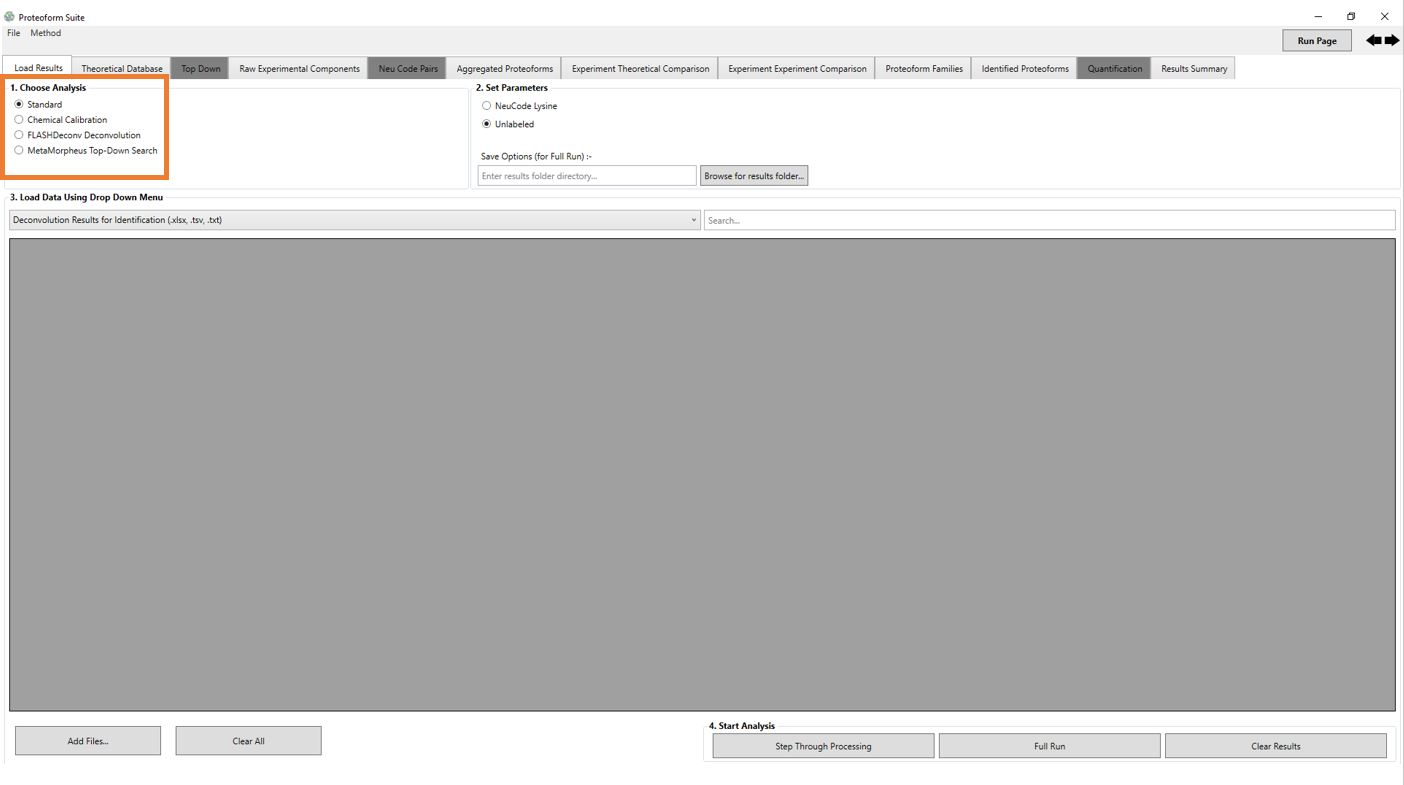
\includegraphics[scale=0.4]{figures/load_results_1.jpg}
\end{figure}

This option selects the type of analysis to perform.
\begin{itemize}
	\item Standard: load in results under standard before navigating through the different pages
	\item Chemical Calibration: calibrate mass and retention time of deconvolution and top-down results (see \textbf{Calibration} section)
	\item FLASHDeconv Deconvolution: deconvolute .mzML files (see \textbf {Deconvolution} section)
	\item MetaMorpheus Top-Down Search: search .mzML or .raw files for list of MS/MS identified proteoforms (see \textbf{Top-Down Search} section)
\end{itemize}

\pagebreak
\subsection{Set Parameters}

\begin{figure}[htbp]
\centering
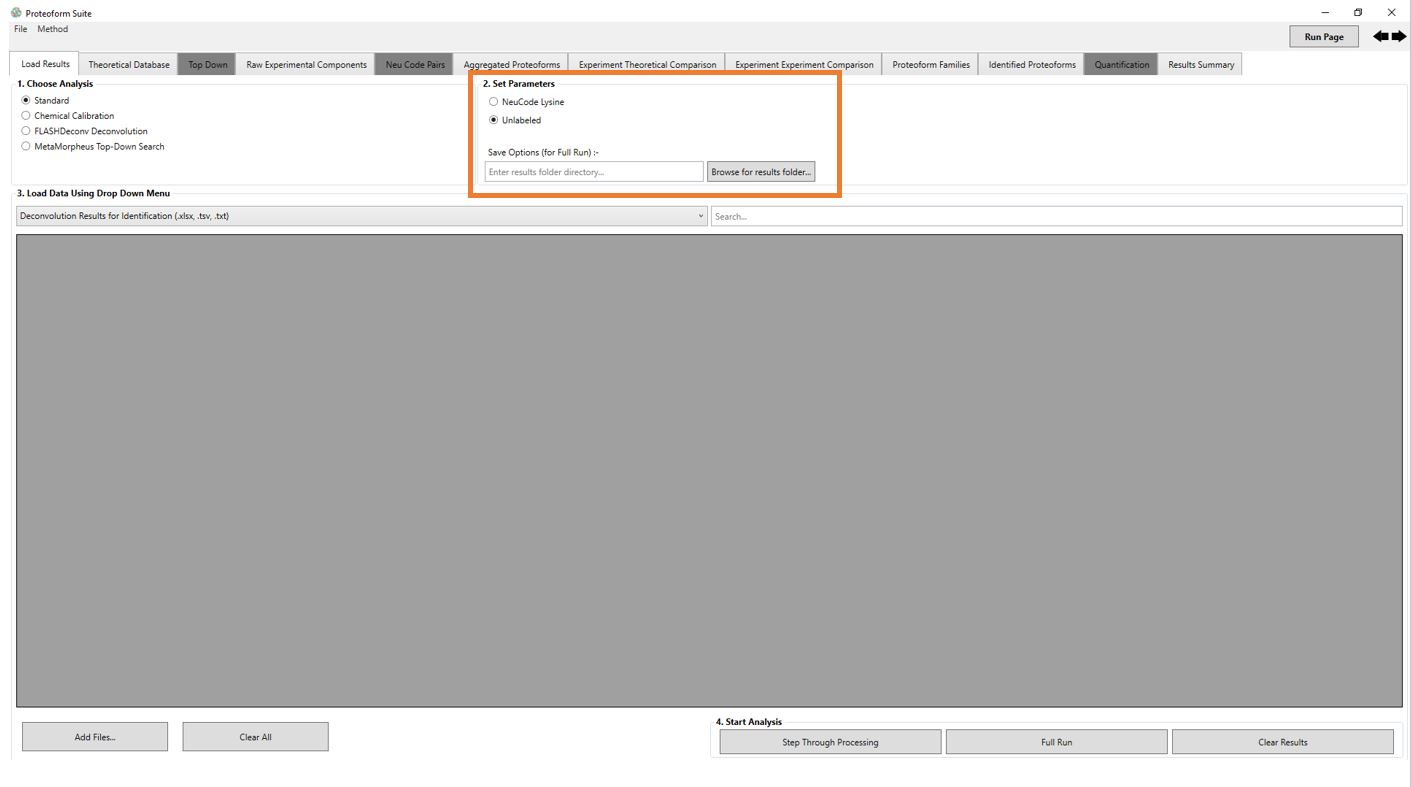
\includegraphics[scale=0.4]{figures/load_results_2.jpg}
\end{figure}

\begin{itemize}
	\item NeuCode Lysine: select if cell culture was performed with heavy and light NeuCode lysine tags 
	\item Unlabeled : select if no labeling was utilized (typical)
	\item Save Options: for full-run of a method .xml file (see below), select a file path to output results
\end{itemize}

\subsection{Load Data Using Drop Down Menu}

\begin{figure}[htbp]
\centering
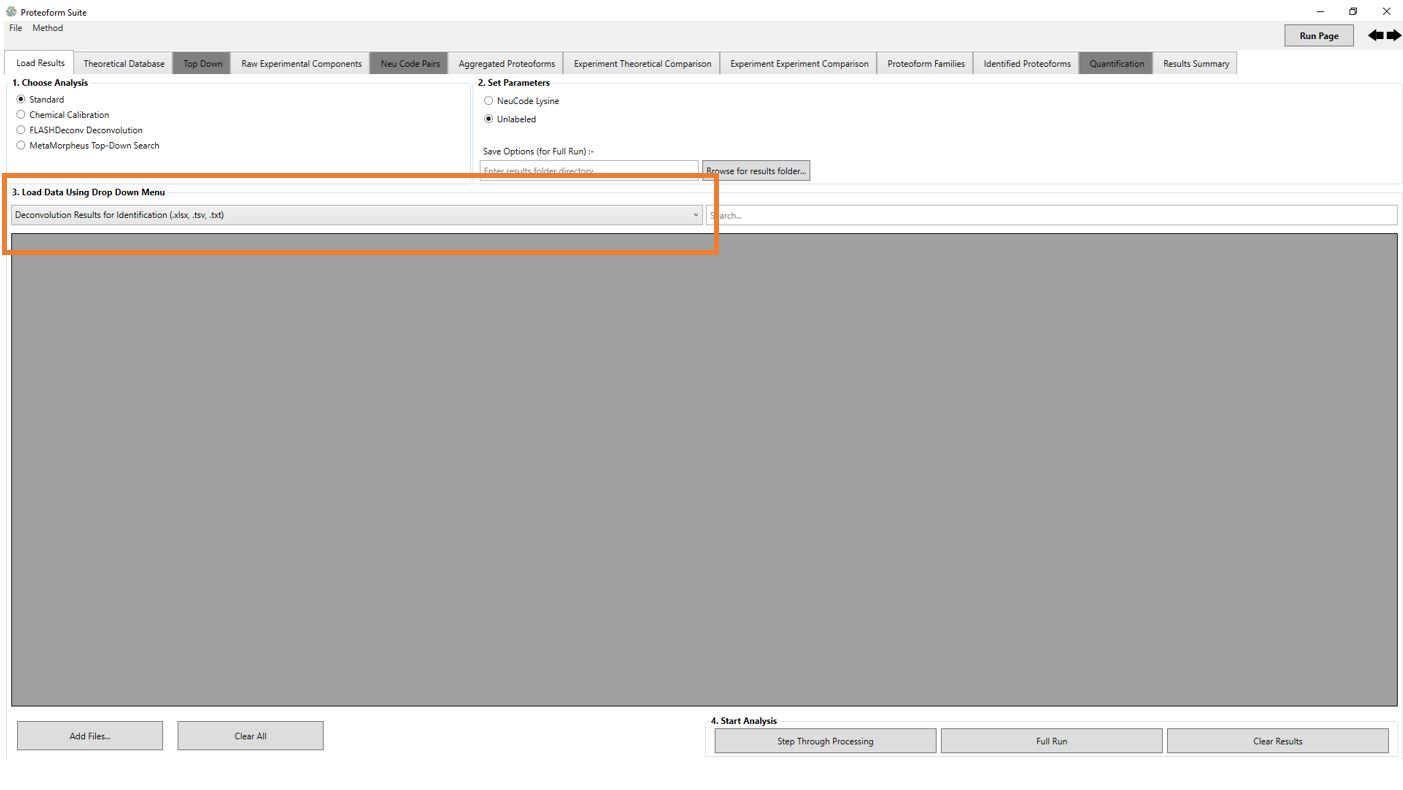
\includegraphics[scale=0.4]{figures/load_results_3.jpg}
\end{figure}

\begin{itemize}
	\item Drop down menu: Change file type to be added by selecting an item in the drop down box. Each file type is described below. 
	\item Add Files...: add files of the type selected in the drop down box
	\item Clear All: clear files of the type selected in the drop down box
\end{itemize}
\pagebreak
\subsection{Deconvolution Results for Identification}

Results from deconvolution of MS1 spectra, \textit{i.e.}, observed proteoform masses. These deconvolution results will be used to identify proteoforms by intact-mass analysis. There are three options for deconvolution results (see \textbf{Deconvolution} section):

\begin{itemize}
	\item Results from Thermo Deconvolution 4.0 (.xlsx)
	\item Results from FLASHDeconv (.tsv)
	\item A three column tab-separated .tsv or .txt file with columns mass, intensity, retention time
\end{itemize}

There is the option to label the Biological Replicate, Fraction, Technical Replicate, and Condition for each file. To change one of these labels for a single file, click the appropriate cell in the table. To change the label for more than one file or cell, select the cells you would like to change the label for, right click your mouse, enter a label, click Okay. 

\subsection{Proteoform Quantification Results}

It is only necessary to enter deconvolution results for quantification if you plan to perform a quantitative analysis of proteoform abundance changes between two conditions (see \textbf{Quantification} section). Results from deconvolution of MS1 spectra, \textit{i.e.}, observed proteoform masses. The proteoform intensity values in these deconvolution results will be used to quantify proteoforms.\supercite{Cesnik2018,Schaffer2018} These results files can be the same or different than the deconvolution results for identification.  There are three options for deconvolution results (see \textbf{Deconvolution} section):

\begin{itemize}
	\item Results from Thermo Deconvolution 4.0 (.xlsx)
	\item Results from FLASHDeconv (.tsv)
	\item A three column tab-separated .tsv or .txt file with columns mass, intensity, retention time
\end{itemize}

To perform a quantification analysis, it is necessary to label the Biological Replicate, Fraction, Technical Replicate, and Condition for each file. The change one of these labels for a single file, click the appropriate cell in the table. To change the label for more than one file or cell, select the cells you would like to change the label for, right click your mouse, enter a label, click Okay. 

\subsection{Protein Databases}

Download a protein database from UniProt (\url{https://www.uniprot.org/proteomes/}). It is recommended to use the Reviewed entries only. A database from MetaMorpheus generated from a bottom-up search and the global post-translational modification discovery strategy (G-PTM-D) can also be utilized.\supercite{Dai2017,Dai2019} Check the contaminant column if the database is a contaminant database. There are two options for protein databases:
\begin{itemize}
\item .xml or .xml.gz: contains annotated PTM information and subsequences
\item .fasta: option to include isoforms when downloaded
\end{itemize}

\subsection{Top-Down Hit Results}

Results from a top-down search of MS/MS spectra, \textit{i.e.}, proteoform identifications. There are two options for top-down results (see \textbf{Top-Down Search} section):
\begin{itemize}
	\item Results from TDPortal (.xlsx)
	\item Results from MetaMorpheus (.psmtsv)
\end{itemize} 

\subsection{MetaMorpheus Bottom-Up Unique Peptides}

Results from a bottom-up search of MS/MS spectra, \textit{i.e.}, peptide identifications.\supercite{Schaffer2020} Download a release of MetaMorpheus and run a bottom-up search (\url{https://github.com/smith-chem-wisc/MetaMorpheus/releases}). In the results folder of the search, load the AllPeptides.psmtsv file. 

\pagebreak
\subsection{Start Analysis}

\begin{figure}[h]
\centering
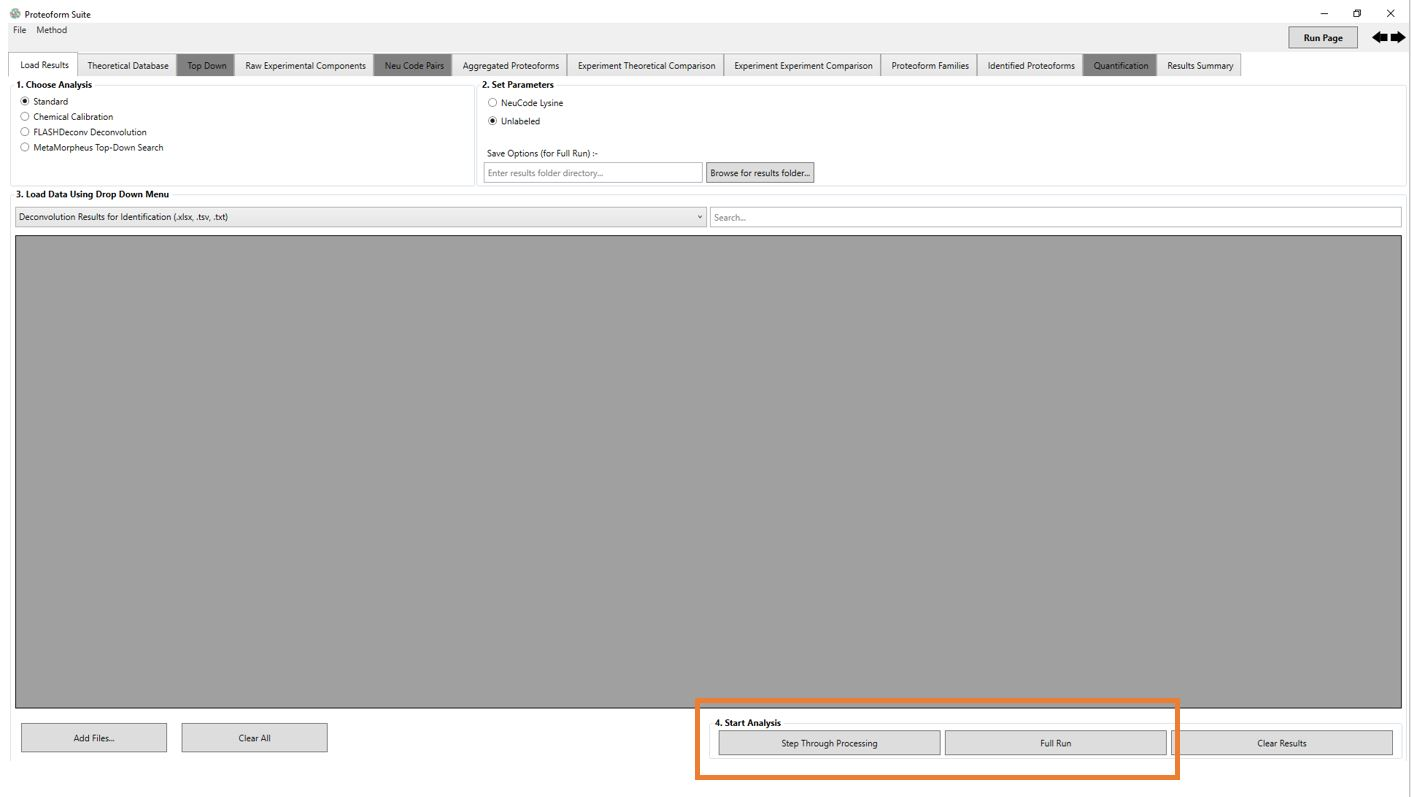
\includegraphics[scale=0.4]{figures/load_results_4.jpg}
\end{figure}

\begin{itemize}
	\item Step Through Processing button: instructions display on how to step through different pages
	\item Full Run button: load in a method .xml or use preset defaults to automatically perform a full run through analysis
	\item Clear Results button: clear all files in the file table
\end{itemize}

\pagebreak
%!TEX root = ../proteoform_suite_manual.tex
%---------------------------------------------------------------------
%	DECONVOLUTION
%---------------------------------------------------------------------

\section{Deconvolution}

Results from deconvolution of MS1 spectra are used to identify proteoforms by intact-mass analysis and to construct proteoform families of observed proteoforms. Deconvolution results are loaded on the Load Results page (see \textbf{Load Results: Standard}) under Deconvolution Results for Identification and Deconvolution Results for Quantification. This section describes how to obtain deconvolution results to import into Proteoform Suite.

\subsection{Thermo Deconvolution 4.0}
\begin{itemize}
\item See Thermo Fisher website for quote and user guide
\item Run Xtract algorithm for high resolution data
\item For each .raw file:
\begin{itemize}
	\item Select Open Results in the Run Queue
	\item Right-click the Results table and choose Export All
	\item Open the .xls file exported and save as a .xlsx file
\end{itemize}
\item The saved .xlsx file is used for Deconvolution Results for Identification and Deconvolution Results for Quantification in the Standard analysis on the Load Results page
\end{itemize}

\subsection{FLASHDeconv}
FLASHDeconv is an ultra-fast deconvolution algorithm for high resolution mass spectrometry data developed by the OpenMS team.\supercite{Jeong2020}
\begin{itemize}
\item On the Load Results page, select FLASHDeconv Deconvolution under Choose Analysis (top left)
\item Input .mzML files into the table (Load Data drop down menu will be set to Spectra Files)
\item FLASHDeconv requires .mzML files. Use MSConvert to convert other file types (\url{http://proteowizard.sourceforge.net/}). Peak picking is NOT recommended.
\item Set Parameters:
\begin{itemize}
\item Min Charge: minimum charge state allowed for deconvolution
\item Max Charge: maximum charge state allowed for deconvolution
\end{itemize}
\item To begin deconvolution, hit the Deconvolute button under Start Analysis (bottom right)
\item For more advanced parameter options, you can also run the command line version of FLASHDeconv, available at \url{https://www.openms.de/comp/flashdeconv/}
\item The resulting .tsv file is used for Deconvolution Results for Identification and Deconvolution Results for Quantification in the Standard analysis on the Load Results page
\end{itemize}

\subsection{Other}
\begin{itemize}
\item If you have another deconvolution algorithm of choice, simply create a three column tab-separated file
\subitem Monoisotopic mass \textbackslash t intensity \textbackslash t retention time
\item This .tsv or .txt file can be used for Deconvolution Results for Identification and Deconvolution Results for Quantification in the Standard analysis on the Load Results page
\end{itemize}
\pagebreak
%!TEX root = ../proteoform_suite_manual.tex
%---------------------------------------------------------------------
%	TOPDOWN SEARCH
%---------------------------------------------------------------------

\section{Top-down Search}

Results from a top-down MS/MS search can be used in Proteoform Suite. These top-down proteoform identifications improve intact-mass analysis and proteoform family construction. Additionally, top-down results can be integrated with bottom-up peptide results. Top-down results are loaded on the Load Results page (see \textbf{Load Results: Standard}) under Top-Down Hit Results. This section describes how to obtain top-down results to import into Proteoform Suite.

\subsection{TDPortal}
TDPortal is a high-throughput global proteome analysis software for top-down data\supercite{LeDuc2004,Zamdborg2007,Toby2019} available through the National Resource for Translational and Developmental Proteomics.
\begin{itemize}
\item Request for access to TDPortal: \url{http://nrtdp.northwestern.edu/tdportal-request/}
\item Download TDViewer to access results: \url{http://topdownviewer.northwestern.edu/}
\item Under Reports tab in TDViewer, export Hit Report
\item The resulting .xlsx file is used for Top-Down Hit Results in the Standard analysis on the Load Results page
\end{itemize}

\subsection{MetaMorpheus}
MetaMorpheus is an MS/MS search software program for both bottom-up and top-down analysis.\supercite{Solntsev2018,Schaffer2019}
\begin{itemize}
\item On the Load Results page, select MetaMorpheus Top-Down Search under Choose Analysis (top left)
\item Load .raw or .mzML files in the table with the Load Data drop down menu set to Spectra Files
\item Load an .xml or .fasta database in the table with the Load Data drop down menu set to Protein Databases
\item Set Parameters:
\begin{itemize}
\item Precursor Mass Tolerance: the difference in mass between the observed precursor and the theoretical proteoform
\item Product Mass Tolerance: the difference in mass between the product ions generated by fragmentation and the theoretical proteoform's theoretical fragmentation spectra
\item Fixed Carbamidomethyl Mod:  fixed modifications are applied to EVERY amino acid in the database specified in the list. Check this box for protein samples that have been reduced and alkylated with iodoacetamide
\item Dissociation Type: the dissociation type used to fragment intact proteoforms and produce product ions for the tandem mass spectra
\end{itemize}
\item To begin the search, hit the MetaMorppheus Top-Down Search button under Start Analysis (bottom right)
\item For more advanced parameter options, you can also run the GUI or command line version of MetaMorpheus, available at \url{https://github.com/smith-chem-wisc/MetaMorpheus/releases}
\item The resulting AllPSMs.psmtsv file is used for Top-Down Hit Results in the Standard analysis on the Load Results page
\end{itemize}

\pagebreak
%!TEX root = ../proteoform_suite_manual.tex
%---------------------------------------------------------------------
%CALIBRATION
%---------------------------------------------------------------------

\section{Calibration}

Calibration is an optional pre-processing step to improve the mass accuracy of the deconvolution and the top-down search results.\supercite{Solntsev2018,Schaffer2018b} High-scoring top-down identifications are used as calibration points. Retention time across files can also be calibrated to correct run-to-run variation. Calibrated deconvolution results are loaded on the Load Results page (see \textbf{Load Results: Standard}) under Deconvolution Results for Identification and Deconvolution Results for Quantification, and calibrated top-down results are loaded on the Load Results page (see \textbf{Load Results: Standard}) under Top-Down Hit Results. This section describes how to perform calibration.

\subsection{Overview}
\begin{itemize}
\item On the Load Results page, select Chemical Calibration under Choose Analysis (top left)
\item Load and label files (see below)
\subitem To change one of these labels for a single file, click the appropriate cell in the table. To change the label for more than one file or cell, select the cells you would like to change the label for, right click your mouse, enter a label, click Okay. 
\item Set parameters (see below)
\item To begin calibration, hit the Calibrate button under Start Analysis (bottom right)
\end{itemize}

\subsection{Load Files}
\begin{itemize}
\item Set the Load Data drop down menu to Spectra Files
\begin{itemize}
\item Add all .raw or .mzML files using the Add Files button or with drag-and-drop
\item Any raw files deconvoluted to generate Deconvolution Results AND searched to generate Top-Down Hit results must be added
\end{itemize}
\item Set the Load Data drop down menu to Uncalibrated Deconvolution Results
\item Add all deconvolution results files using the Add Files button or with drag-and-drop
\item Set the Load Data drop down menu to Uncalibrated Top-Down Hit Results
\item Add all top-down results files using the Add Files button or with drag-and-drop
\item Label the Biological Replicate, Fraction, Technical Replicate, and Condition for each file. 
\begin{itemize}
	\item Each spectra file and deconvolution result file must have a different label
	\item Each spectra file label should exactly match the corresponding deconvolution result label
	\item Calibration is performed across technical replicates for the same biological replicate, fraction, and condition. Therefore, if you wish to have a top-down file calibrate an intact-mass file, it is necessary to have the biological replicate, fraction, and condition match while the technical replicate label varies (ex: 1, 2, 3, etc.)
\end{itemize}
\end{itemize}

\subsection{Set Parameters}
\begin{itemize}
\item NeuCode Lysine: select if cell culture was performed with heavy and light NeuCode lysine tags 
\item Unlabeled : select if no labeling was utilized (typical)
\item Write Calibrate Raw Files: if checked, calibrated .mzML files will be exported in the same file location as the original spectra files
\item Calibrate Top-Down Files: if checked, a calibrated top-down results file will be exported in the same file location as the original top-down results file
\item Calibrate Masses: if checked, calibration will be performed on proteoform masses
\item Mass Tol. (ppm): mass tolerance used for mass calibration if Calibrate Masses is checked
\item Calibrate Retention Times: if checked, calibration will be performed on proteoform retention times
\item RT Tol. (min): retention time tolerance used for retention time calibration if Calibrate Retention Times is checked
\end{itemize}


\pagebreak
%!TEX root = ../proteoform_suite_manual.tex
%---------------------------------------------------------------------
%	THEORETICAL DATABASE
%---------------------------------------------------------------------

\section{Theoretical Database}

\subsection{Overview}
On this page, theoretical proteoforms are created using the file(s) loaded under Protein Databases on the Load Results page. This theoretical proteoform database includes theoretical proteoforms with combinations of annotated post-translational modifications (PTMs) and subsequences. Theoretical proteoforms are used in intact-mass analysis to identify proteoforms (see \textbf{Experiment-Theoretical Comparison} section). Decoy databases are also generated to compute a false discovery rate for intact-mass proteoform identifications. The modifications table (bottom right) enables a user to edit modifications.  The bottom-up result file(s) loaded under MetaMorpheus Bottom-Up Unique Peptides on the Load Results Page is used to create a list of bottom-up peptides, which are integrated with theoretical proteoforms. 

\subsection{Run Page}
\begin{itemize}
\item Load database file(s) on the Load Results page under Protein Databases (see \textbf{Load Results} section)
\item Set all parameters as desired for current analysis (see below)
\item Click Run Page button (top right)
\end{itemize}

\subsection{Set Parameters}
\begin{figure}[h]
\centering
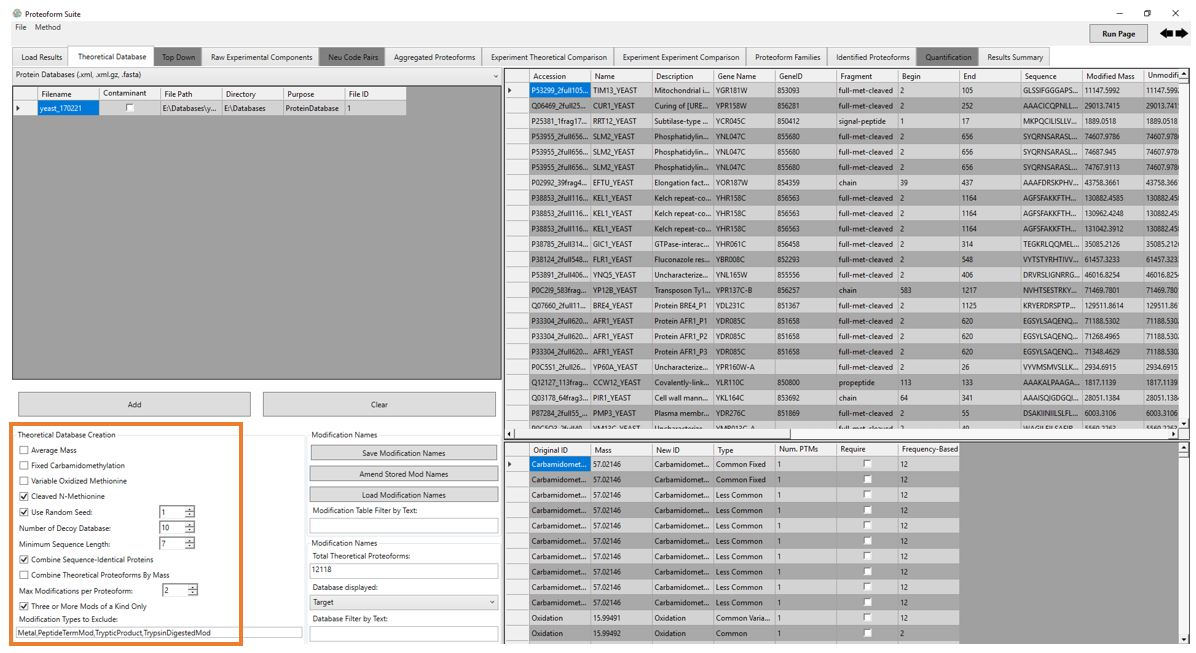
\includegraphics[scale=0.43]{figures/theoretical1.jpg}
\end{figure}
\begin{itemize}
\item Average Mass: if checked, the average mass of each theoretical proteoform will be used instead of the default monoisotopic mass
\item Fixed Carbamidomethylation: if checked, each cysteine on each theoretical proteoform will have a carbamidomethylation group added
\item Variable Oxidized Methionine: if checked, theoretical proteoforms will be added with oxidation modifications up to the number of methionine residues/the Max Modifications per Proteoform parameter setting
\item Cleaved N-Methionine: if checked, methionine will be cleaved off of each full sequence (subsequences UniProt containing the N-methionine will still be added)
\item Use Random Seed: a random seed will be used in the random number generator creating decoy databases, resulting in the same decoy database each time (with the same given parameters)
\item Random Seed: this number will be used for the random seed if the Use Random Seed box is checked
\item Number of Decoy Databases: the number of decoy databases generated. The average across each decoy database result is used to compute the false discovery rate for intact-mass identifications
\item Minimum Sequence Length: the minimum length of a theoretical proteoform in the database
\item Combine Sequence-Identical Proteins: if checked, sequences that are the same from different genes/proteins will be combined into a single theoretical proteoform entry
\item Combine Theoretical Proteoforms by Mass: if checked, different proteoforms with the same mass (up to 4 decimal places) will be combined into a single theoretical proteoform entry
\item Max Modifications per Proteoform: theoretical proteoforms will be generated for each UniProt protein entry containing annotated modifications in different combinations up to this number
\item Three or More Mods of a Kind Only: if checked, modification combinations with different modifications will only go up to 2 modifications per theoretical proteoform. If Max Modifications per Proteoform is set to greater than 2, only modification combinations containing annotated modifications of the same type (ex: triphospho) will go from three modifications up to this number
\item Modification Types to Exclude: comma-separated list of types of modifications to exclude for annotated modifications in the database
\pagebreak
\item Modification Names table: the bottom right table displays each input modification. Several columns can be edited in this table:
\begin{figure}[htbp]
\centering
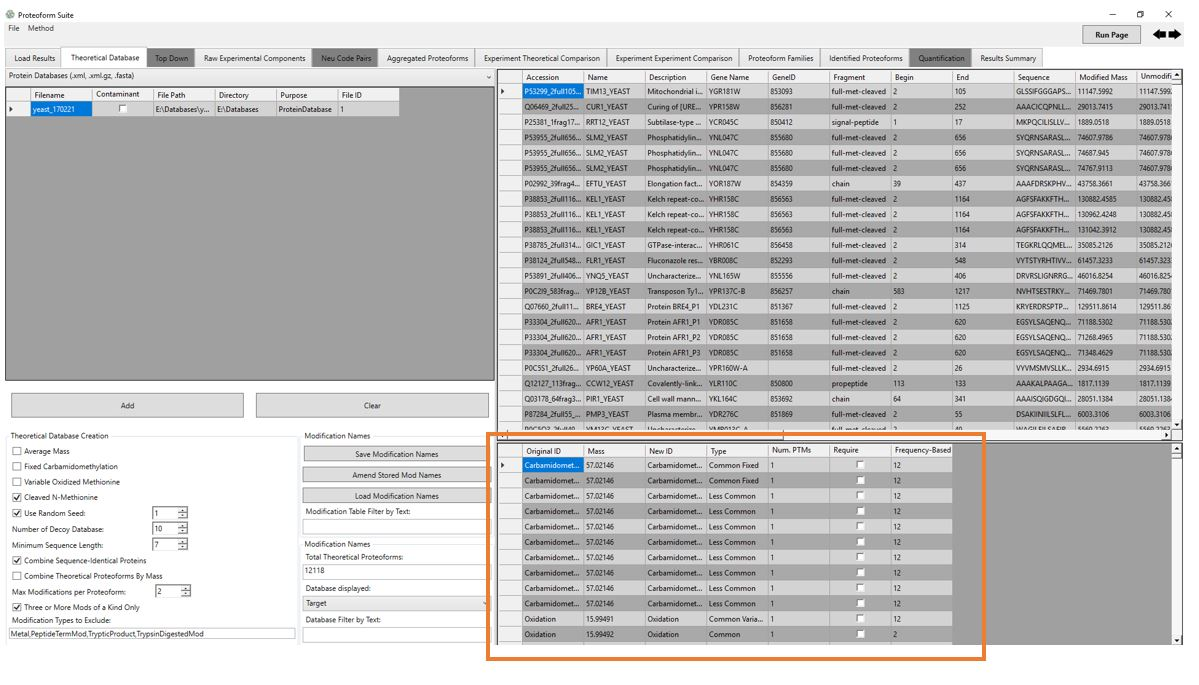
\includegraphics[scale=0.43]{figures/theoretical.jpg}
\end{figure}
\begin{itemize}
\item New ID: the unlocalized version of the modification name, used in Proteoform Suite intact-mass analysis
\item Num. PTMs Represented: the number of PTMs represented by this PTM entry (ex: Dimethylation - 2 PTMs)
\item Require Proteoform Without This Modification: if checked, a proteoform is only identified containing this modification if a proteoform without this modification is also identified. Potentially useful for modifications such as adducts
\item Frequency-Based Rank of PTM Mass: this rank is used in intact-mass analysis to favor more common modifications (lower number is prioritized).
\end{itemize}
\item Save Modification Names: saves a new .modnames file with edits in Modification Names table
\item Amend Stored Mod Names: saves and overwrites .modnames file used in Proteoform Suite
\item Load Modification Names: load a new .modnames file for use in current analysis
\item Modification Table Filter by Text: filter the Modification Names table (bottom right) by any entered text
\end{itemize}

\subsection{Results}

\begin{itemize}
	\item Theoretical Proteoforms table: the top right table displays all theoretical proteoforms generated
	\begin{figure}[h]
\centering
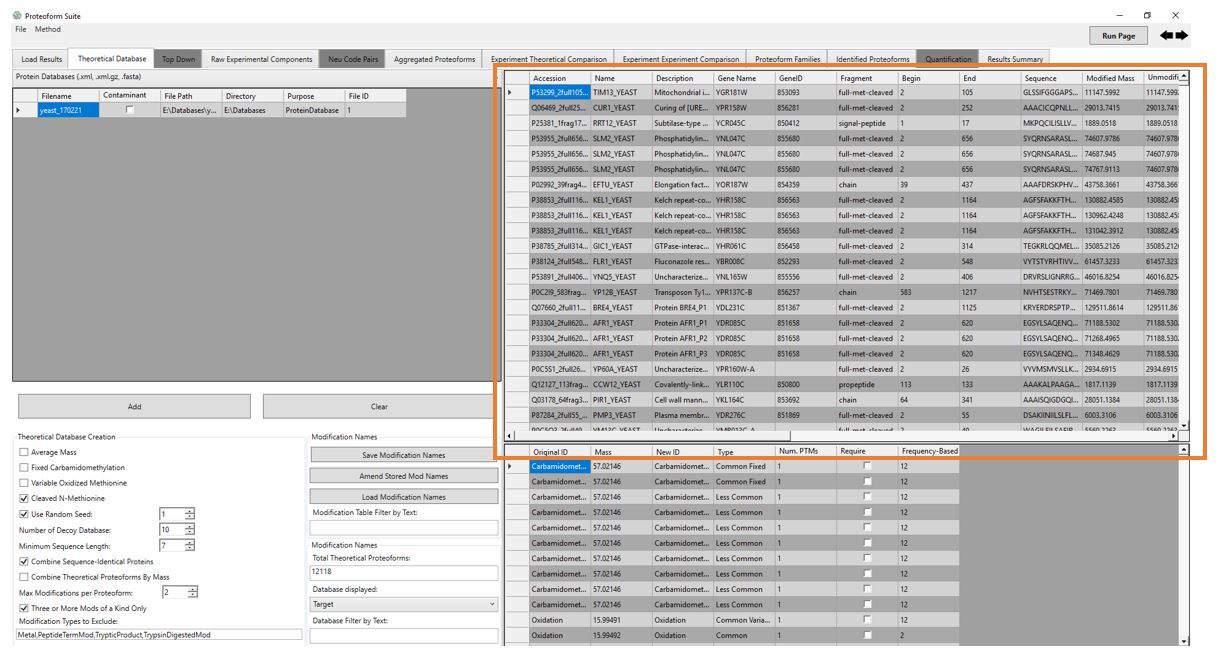
\includegraphics[scale=0.42]{figures/theoretical2.jpg}
\end{figure}
	\begin{itemize}
		\item Accession: accession given by Proteoform Suite for this specific theoretical proteoform
		\item Name: protein name from UniProt
		\item Description: protein description from UniProt
		\item Gene Name: gene name from UniProt
		\item GeneID: gene ID from UniProt
		\item Fragment: sequence description
		\item Begin: theoretical proteoform begin residue in protein full sequence in UniProt
		\item End: theoretical proteoform end residue in protein full sequence in UniProt
		\item Sequence: theoretical proteoform sequence
		\item Modified Mass: monoisotopic (or average) mass of theoretical proteoform with any modifications
		\item Unmodified Mass: monoisotopic (or average) mass of theoretical proteoform without modifications
		\item PTM Mass: mass of PTMs on theoretical proteoform
		\item Contaminant: checked if theoretical proteoform is from contaminant database
		\item Lysine Count: number of lysines in theoretical proteoform sequence
		\item PTM Description: PTMs on theoretical proteoform
		\item GO Term IDs: Gene Ontology term IDs from UniProt
		\item Grouped Accessions: accession grouped if Combine Sequence-Identical Proteins and/or Combine Theoretical Proteoforms By Mass are checked
		\item Top-Down Theoretical: theoretical proteoform identified by top-down analysis (must run Top-Down page first)
		\item Not in Original Database: theoretical proteoform added because of top-down identification, not in original database pre-top-down-analysis (must run Top-Down page first)
		\item Bottom-Up PSMs Count: number of bottom-up PSMs derived from this theoretical proteoform
		\item Peptide-Specific Modified Bottom-Up PSMs: modified residues confirmed ID'd by bottom-up peptides derived from this theoretical proteoform, keeping unique peptidoforms separate
		\item Modified Bottom-Up PSMs: modified residues confirmed by ID'd bottom-up peptides derived from this theoretical proteoform
		\item Bottom-Up Evidence for All PTMs: checked if all PTMs on this theoretical proteoform are confirmed by at least one modified bottom-up peptide
		\item Bottom-Up Evidence for Begin: checked if bottom-up peptide identified with begin residue at this theoretical proteoform's begin residue
		\item Bottom-Up Evidence for End: checked if bottom-up peptide identified with end residue at this theoretical proteoform's end residue
	\end{itemize}
	\item Total Theoretical Proteoforms: number of theoretical proteoforms generated
	\item Database displayed: which database is displayed (target or decoy database)
	\item Database filter by Text: filter the Theoretical Proteoforms table (top right) by any entered text
		\begin{figure}[h]
\centering
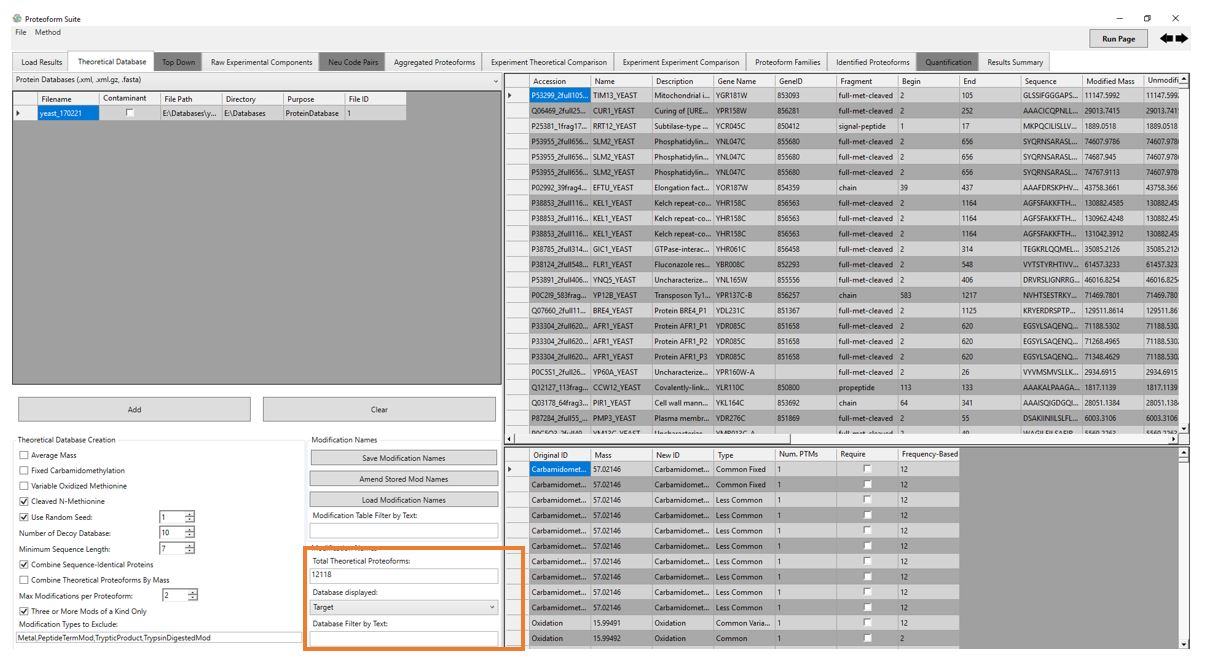
\includegraphics[scale=0.42]{figures/theoretical3.jpg}
\end{figure}
\end{itemize}

\pagebreak
%!TEX root = ../proteoform_suite_manual.tex
%---------------------------------------------------------------------
%	TOPDOWN
%---------------------------------------------------------------------

\section{Top-Down}

\subsection{Overview}
On this page, the top-down hit results are read in from the file(s) loaded under Top-Down Hit Results on the Load Results page. A top-down hit is a proteoform spectral match. Top-down hits are then aggregated into top-down  proteoforms by identification and retention time. The theoretical database is supplemented with top-down proteoform identifications not already present in the database. Bottom-up peptide results are integrated with the top-down proteoform results.

\subsection{Run Page}
\begin{itemize}
\item Load top-down results file(s) on the Load Results page under Top-Down Hit Results (see \textbf{Load Results} section)
\item Set all parameters as desired for current analysis (see below)
\item Click Run Page button (top right)
\end{itemize}

\subsection{Set Parameters}
\begin{figure}[h]
\centering
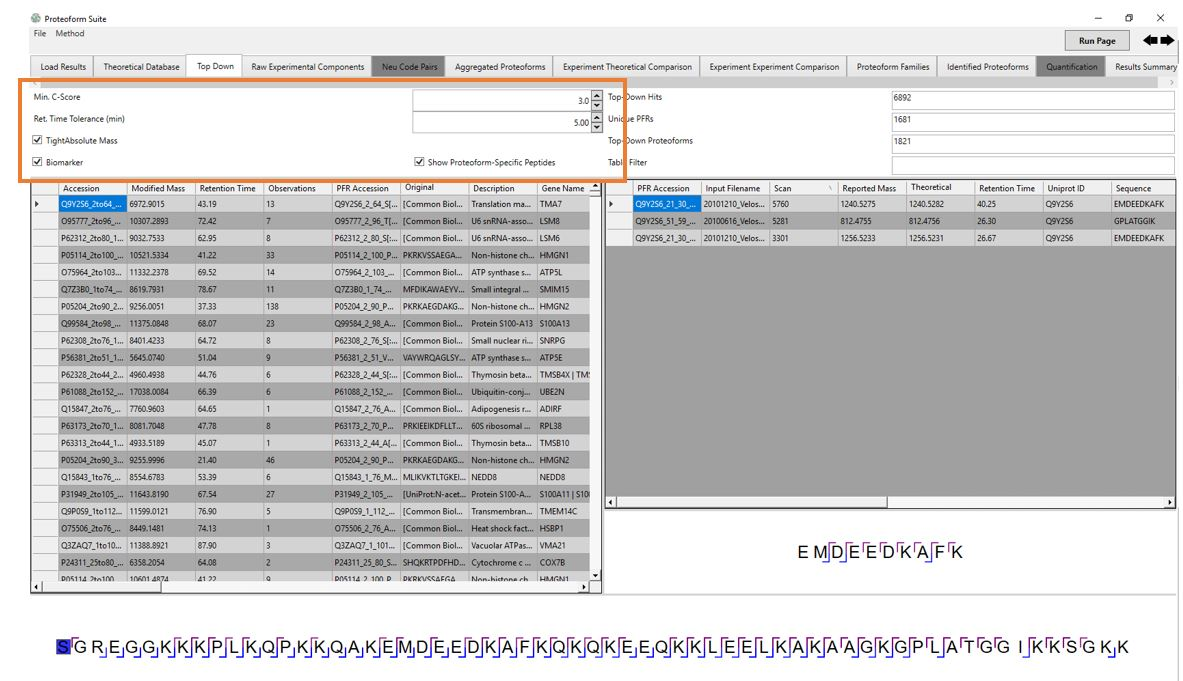
\includegraphics[scale=0.42]{figures/topdown1.jpg}
\end{figure}
\begin{itemize}
\item Min. C-Score: the minimum C-score\supercite{LeDuc2014} for TDPortal results required for a top-down hit to be included. C-scores of 3 and higher correspond to identified proteoforms and C-scores of 40 and higher correspond to well-characterized proteoforms
\item Ret. Time Tolerance (min): retention time tolerance used for aggregated top-down hits of the same proteoform identifications. Top-down hits of the same ID that elute outside of this tolerance will be aggregated into separate top-down proteoforms
\item Tight Absolute Mass: if checked, TDPortal hits from the Tight Absolute Mass search will be included
\item Biomarker: if checked, TDPortal hits from the Biomarker search will be included
\end{itemize}

\subsection{Results}
\begin{itemize}
	\item Top-Down Hits: total number of top-down hits (proteoform spectral matches)
	\item Unique PFRs: unique proteoform identifications
	\item Top-Down Proteoforms: number of aggregated top-down proteoforms. May be greater than the number of unique PFRs if some hits of the same ID fall outside of the retention time tolerance
	\item Table Filter: filter the Top-Down Proteoforms table (left) by any entered text
		\begin{figure}[h]
\centering
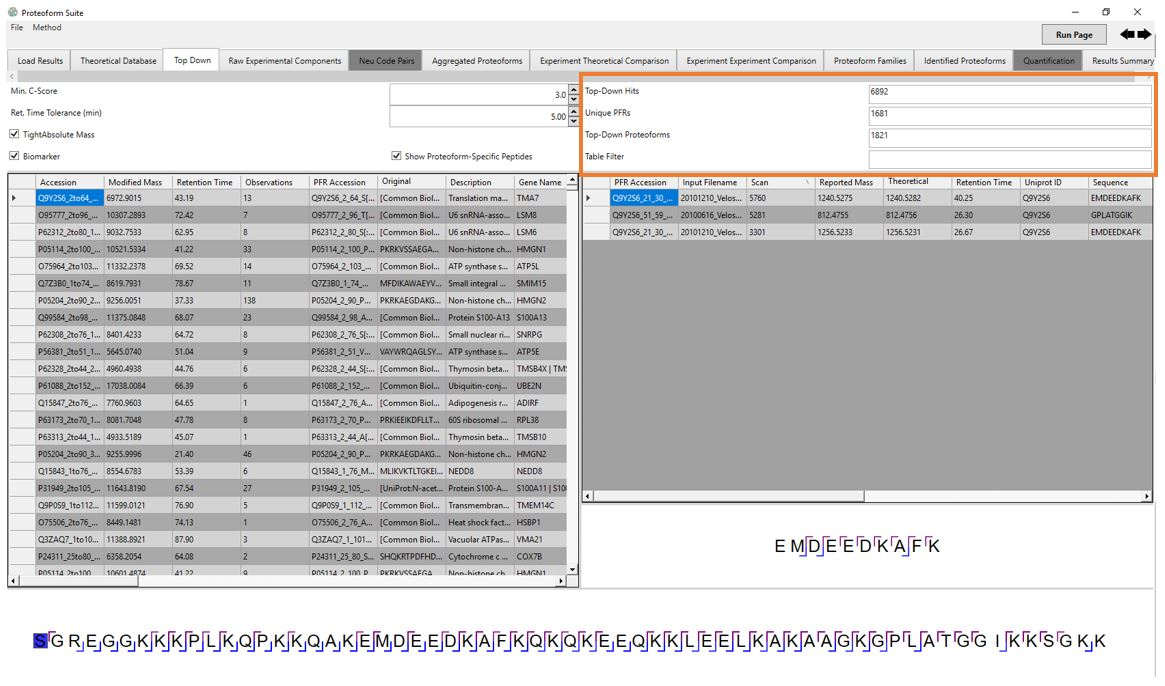
\includegraphics[scale=0.42]{figures/topdown2.jpg}
\end{figure}
	\newpage
	\item Top-down Proteoforms table: the left table displays all top-down proteoforms. For MetaMorpheus results, ambiguous identifications in a single top-down proteoform have information separated by a "|". 
	\begin{figure}[h]
\centering
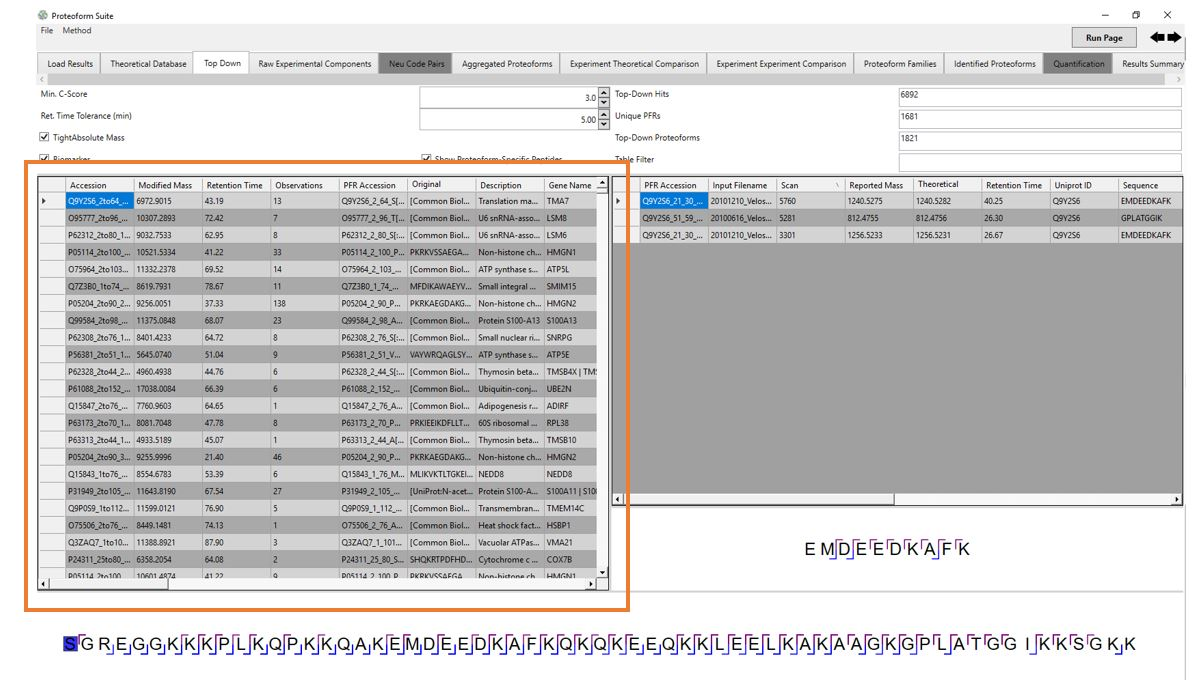
\includegraphics[scale=0.42]{figures/topdown3.jpg}
\end{figure}
	\begin{itemize}
		\item Accession: accession given by Proteoform Suite for this specific top-down proteoform
		\item Modified Mass: monoisotopic mass of top-down proteoform (average of aggregated top-down hits)
		\item Retention Time: retention time of top-down proteoform (average of aggregated top-down hits)
		\item Observations: number of aggregated top-down hits in this top-down proteoform
		\item PFR Accession: protein accession\_begin residue\_end residue\_full sequence with PTMs
		\item Original PFR Accession/full-sequence: PFR accession in TDPortal, full sequence reported in MetaMorpheus
		\item Description: protein description from UniProt
		\item Gene Name: gene name from UniProt
		\item UniProt ID: protein UniProt ID
		\item Accessions: UniProt protein accession
		\item PTM Description: PTMs on top-down proteoform
		\item Begin and End: top-down proteoform begin and end residue in protein full sequence in UniProt
		\item Sequence: top-down proteoform sequence
		\item UniProt-Annotated Modifications: all UniProt annotated residues for PTMs on this top-down proteoform in UniProt database provided
		\item Potentially Novel Mods: checked if this top-down proteoform contains PTMs not annotated in UniProt database provided
		\item Best Hit Score: best C-score (TDPortal) or MetaMorpheus score (MetaMorpheus) out of aggregated hits for this top-down proteoform
		\item Best Hit Delta Score: best delta score (score difference between next best scoring identification) out of aggregated hits for this top-down proteoform (MetaMorpheus results only)
		\item Level: proteoform identification level based on five-level scheme\supercite{Smith2019b}
		\item Level Description: description of proteoform level assignment (sources of ambiguity)
		\item Mass Error: difference in mass between experimental and theoretical proteoform monoisotopic mass
		\item Best Hit Info: filename for highest scoring hit aggregated into this top-down proteoform
		\item Family: proteoform family number (must have run through full Proteoform Suite analysis)
		\item Linked Proteoform References: proteoforms in family network path of identification to the nearest theoretical proteoform (must have run through full Proteoform Suite analysis)
		\item Bottom-Up PSMs Count: number of bottom-up PSMs derived from this top-down proteoform
		\item Different Ambiguity in Bottom-Up PSMs: checked for ambiguous top-down identifications where the different IDs have a different number of bottom-up PSMs
		\item Modified Bottom-Up PSMs: modified residues confirmed by ID'd bottom-up peptides derived from this top-down proteoform
		\item All Modified Bottom-Up PSMs from Protein: modified residues confirmed by ID'd bottom-up peptides derived from this top-down proteoform's protein
		\item Bottom-Up PSMs Separate Peptides: modified residues confirmed ID'd by bottom-up peptides derived from this top-down proteoform, keeping unique peptidoforms separate
		\item Bottom-Up Evidence for Begin: checked if bottom-up peptide identified with begin residue at this top-down proteoform's begin residue
		\item Bottom-Up Evidence for End: checked if bottom-up peptide identified with end residue at this top-down proteoform's end residue
		\item Bottom-Up Evidence for All PTMs: checked if all PTMs on this top-down proteoform are confirmed by at least one modified bottom-up peptide
		\item Sequence Specific: description of difference in PTMs between bottom-up peptides from this top-down proteoform sequence and this top-down proteoform's PTMs
		\item All Peptides from Protein: description of difference in PTMs between bottom-up peptides from this top-down proteoform's protein and this top-down proteoform's PTMs
		\item Fragments: if MetaMorpheus results, MS/MS fragments identified
	\end{itemize}
		\begin{figure}[h]
\centering
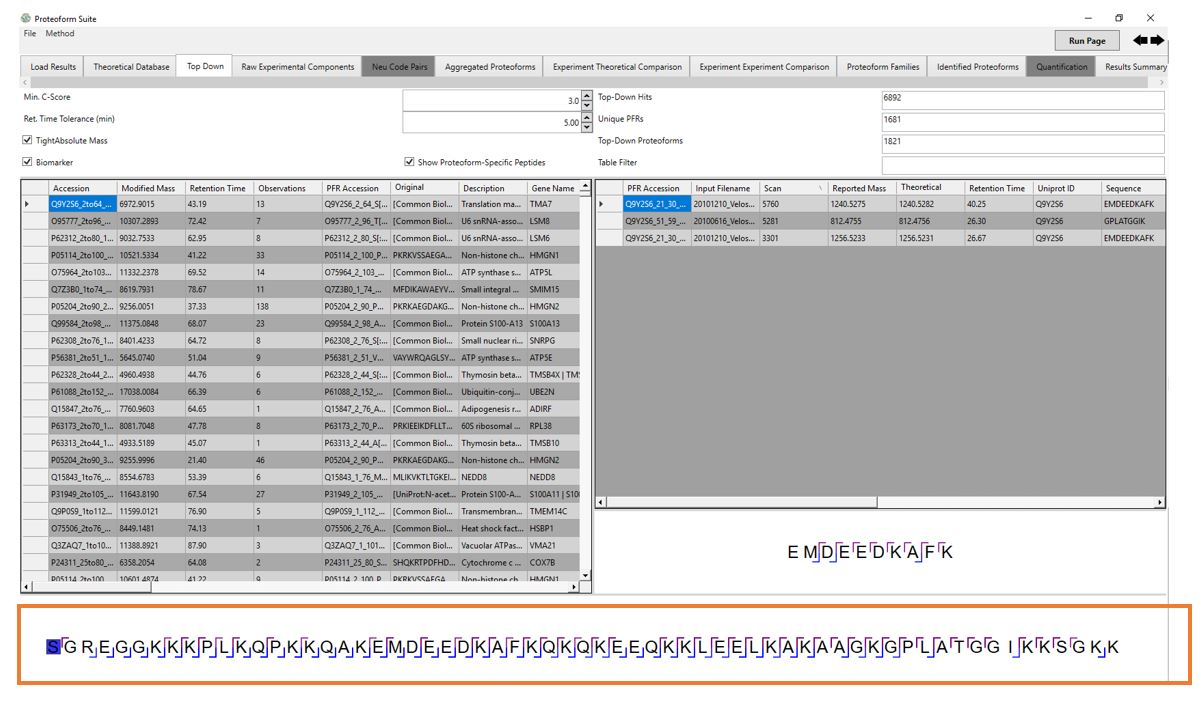
\includegraphics[scale=0.42]{figures/topdown4.jpg}
\end{figure}
	\item Top-down Proteoform Sequence box: bottom box on page where sequence is displayed with PTMs for the top-down proteoform selected in the Top-Down Proteoforms table (left). If MetaMorpheus results, sequence is annotated based on identified MS/MS fragments
	\item Show Proteoform-Specific Peptides: if checked, only peptides specific to the selected top-down proteoform in the Top-Down Proteoform table (left) are displayed in the Bottom-Up Peptide table (right). If unchecked, all bottom-up peptides from the top-down proteoform's protein are displayed. 
	\item Bottom-Up Peptides table: the right table displays bottom-up peptides from the top-down proteoform selected in the Top-Down Proteoforms table (left) if Show Proteoform-Specific Peptides is checked. The right table displays all bottom-up peptides from the top-down proteoform's protein selected in the Top-Down Proteoforms table (left) if Show Proteoform-Specific Peptides is unchecked. 
	\begin{figure}[h]
\centering
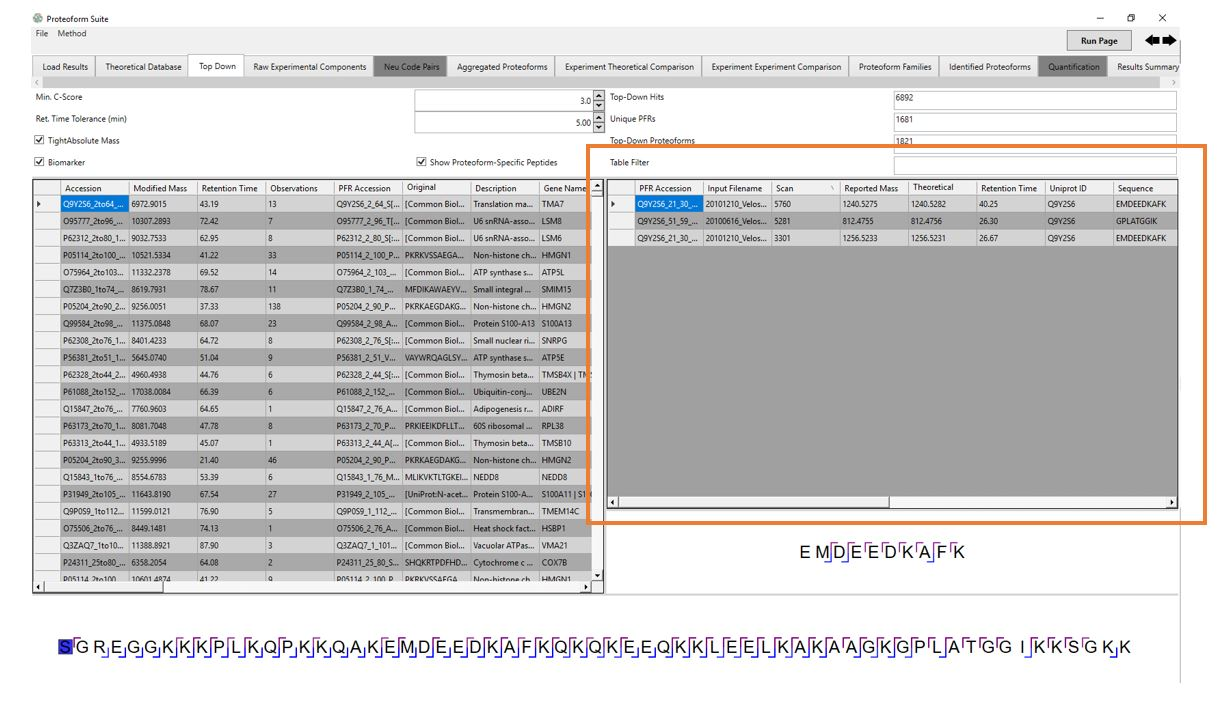
\includegraphics[scale=0.42]{figures/topdown5.jpg}
\end{figure}
	\begin{itemize}
		\item PFR Accession: protein accession\_begin residue\_end residue\_full sequence with PTMs
		\item Input Filename: filename for this bottom-up peptide identification
		\item Scan: scan number for this bottom-up peptide identification
		\item Reported Mass: observed monoisotopic mass for this bottom-up peptide identification
		\item Theoretical Mass: theoretical mass for this bottom-up peptide identification
		\item Retention Time: retention time for this bottom-up peptide identification
		\item UniProt ID: protein UniProt ID
		\item Sequence: peptide sequence
		\item Begin: peptide begin residue in protein full sequence in UniProt
		\item End: peptide end residue in protein full sequence in UniProt
		\item PTM Description: PTMs on peptide
		\item Accession: UniProt protein accession
		\item Name: name of protein from UniProt
		\item Q-value: PEP q-value for this bottom-up peptide
		\item Score: MetaMorpheus score for this peptide
		\item Shared: checked if this peptide is a shared peptide between multiple proteins
	\end{itemize}
	\item Bottom-Up Sequence box: middle right box on page where sequence is displayed with PTMs for the peptide selected in the Bottom-Up Peptides table (right). If MetaMorpheus results, sequence is annotated based on identified MS/MS fragments
	\begin{figure}[h]
\centering
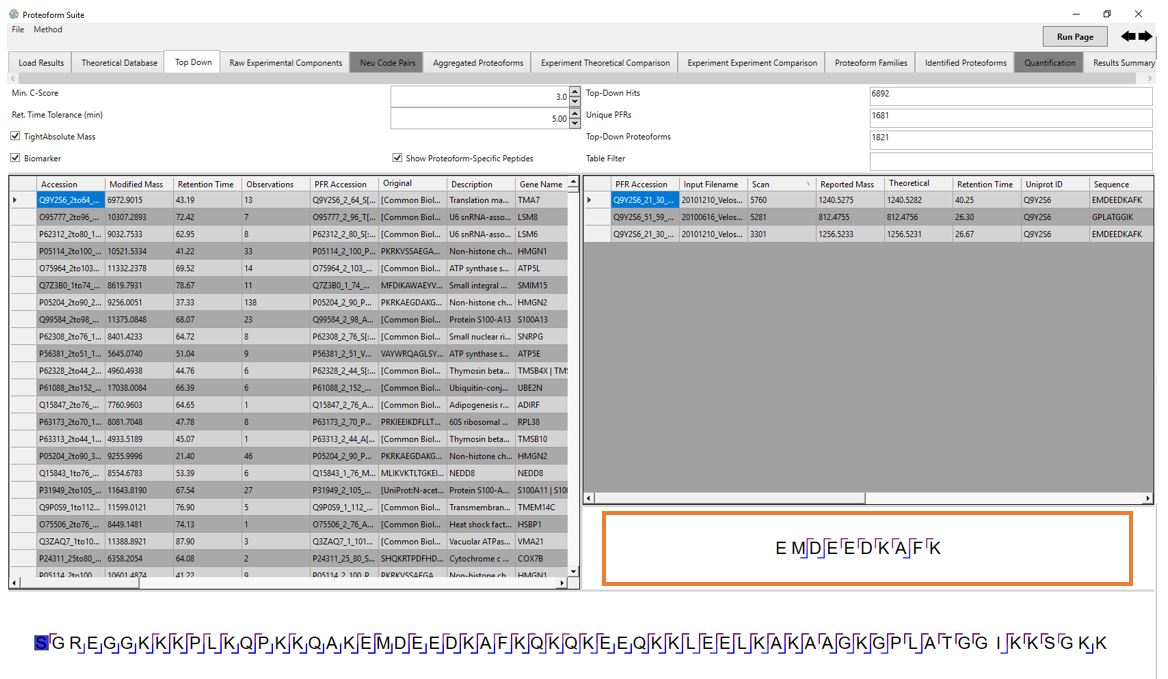
\includegraphics[scale=0.42]{figures/topdown6.jpg}
\end{figure}
\end{itemize}
\pagebreak
%!TEX root = ../proteoform_suite_manual.tex
%---------------------------------------------------------------------
%	RAW EXPERIMENTAL COMPONENTS
%---------------------------------------------------------------------

\section{Raw Experimental Components}


\subsection{Overview}

On this page, raw experimental components are read in from the file(s) loaded under Deconvolution Results for Identification and Deconvolution Results for Quantification on the Load Results page. A raw experimental component is an individual proteoform observation as reported in the deconvolution results file(s). 

\subsection{Run Page}
\begin{itemize}
\item Load the deconvolution results file(s) on the Load Results page under Deconvolution Results for Identification. If desired, label the biological replicate, fraction, technical replicate, and condition for each file (see \textbf{Load Results} section)
\item If performing a quantitative analysis, load the deconvolution results file(s) on the Load Results page under Deconvolution Results for Quantification. Label the biological replicate, fraction, technical replicate, and condition for each file (see \textbf{Load Results} section)
\item Set all parameters as desired for current analysis (see below)
\item Click Run Page button (top right)
\end{itemize}

\subsection{Set Parameters}
\begin{figure}[h]
\centering
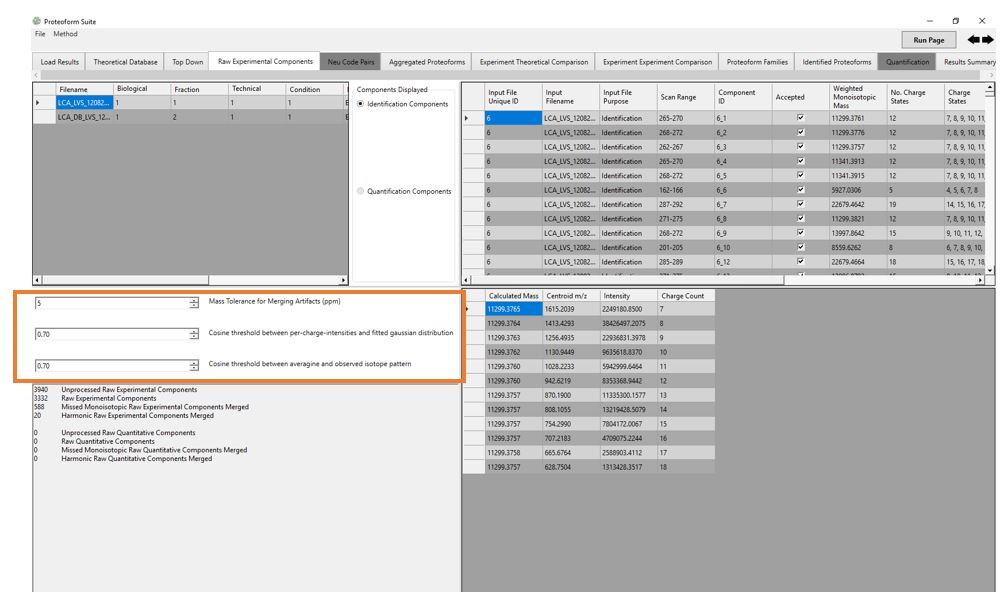
\includegraphics[scale=0.5]{figures/rawcomponents1.jpg}
\end{figure}
\begin{itemize}
\item Mass tolerance for Merging Artifacts (ppm): mass tolerance used to merge deconvolution artifacts including missed monoisotopic mass differences and charge state harmonics
\item Cosine threshold between per-charge intensities and fitted gaussian distribution: minimum value as described for FLASHDeconv deconvolution results
\item Cosine threshold between averagine and observed isotope pattern: minimum value as described for FLASHDeconv deconvolution results
\end{itemize}
\subsection{Results}
\begin{itemize}
	\item Unprocessed Raw Experimental Components: the number of raw experimental components for identification before merging artifacts
	\item Raw Experimental Components: the number of raw experimental components for identification after merging artifacts
	\item Missed Monoisotopic Raw Experimental Components Merged: the number of raw experimental components for identification artifacts merged due to being missed monoisotopic errors within the set mass tolerance
	\item Harmonic Raw Experimental Components Merged: the number of raw experimental components for identification artifacts merged due to being charge state harmonic errors within the set mass tolerance
	\item Unprocessed Raw Quantitative Components: the number of raw experimental components for quantification before merging artifacts
	\item Raw Quantitative Components: the number of raw experimental components for quantification after merging artifacts
	\item Missed Monoisotopic Raw Quantitative Components Merged: the number of raw experimental components for quantification artifacts merged due to being missed monoisotopic errors within the set mass tolerance
	\item Harmonic Raw Quantitative Components Merged: the number of raw experimental components for quantification artifacts merged due to being charge state harmonic errors within the set mass tolerance
	\begin{figure}[h]
\centering
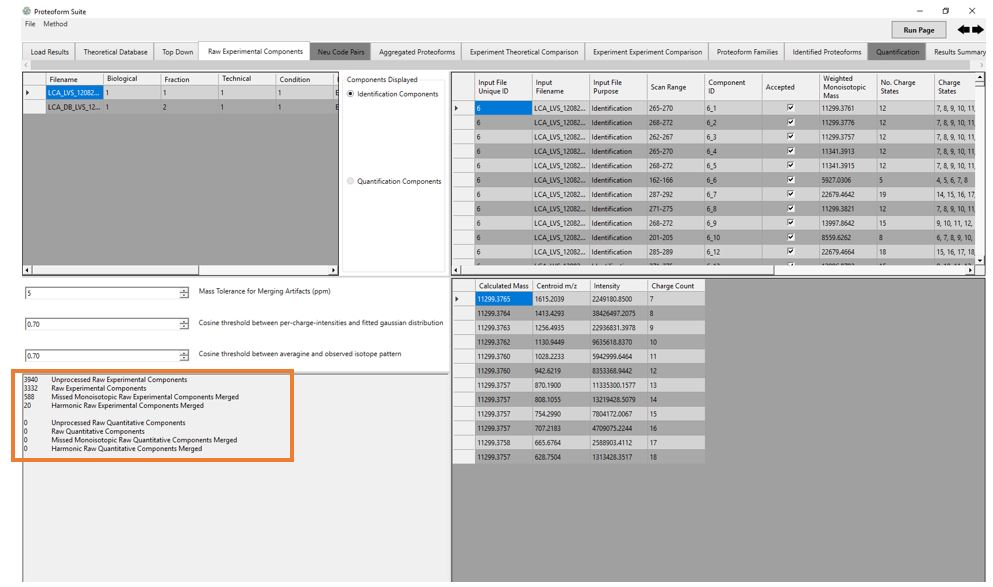
\includegraphics[scale=0.5]{figures/rawcomponents2.jpg}
\end{figure}
\pagebreak
	\item Raw Experimental Components table: the top right table displays raw experimental components for either Identification or Quantification (depending on selection of Components Displayed to the left of the table)
		\begin{figure}[h]
\centering
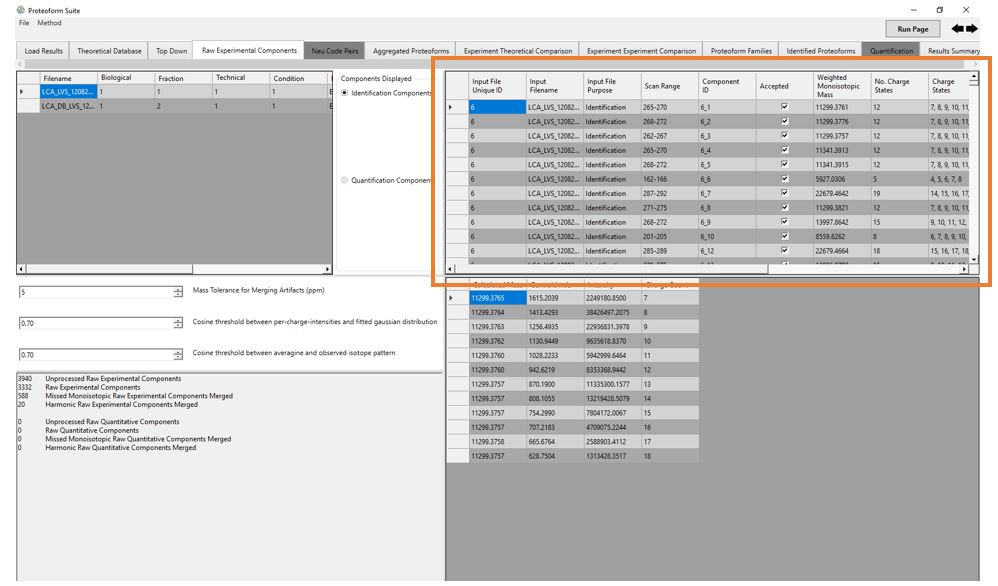
\includegraphics[scale=0.5]{figures/rawcomponents3.jpg}
\end{figure}
	\begin{itemize}
		\item Input File Unique ID: file ID number for filename of Deconvolution Results for Identification or Quantification for this raw experimental component
		\item Input Filename: filename of Deconvolution Results for Identification or Quantification for this raw experimental component
		\item Input File Purpose: either Identification or Quantification
		\item Scan Range: MS scan range for this raw experimental component
		\item Component ID: Proteoform Suite given ID for this raw experimental component; file ID\_component \#
		\item Accepted: checked if this raw experimental component is accepted for analysis
		\item Weighted Monoisotopic Mass: monoisotopic mass of raw experimental component weighted by intensity of each charge state (more intense charge states are higher weighted)
		\item No. Charges: number of charge states for this raw experimental component
		\item Charge States: comma-separated list of charge states for this raw experimental component
		\item Intensity Sum: intensity of this raw experimental component, charge state normalized
		\item RT Range: retention time range
		\item Apex RT: apex retention time as reported
		\item Reported Monoisotopic Mass: monoisotopic mass reported by deconvolution input
		\item Reported Intensity: intensity reported by deconvolution input
	\end{itemize}
	\item Charge States table: the bottom right table displays all charge states from the raw experimental component selected in the Raw Experimental Components table (top right)
		\begin{figure}[h]
\centering
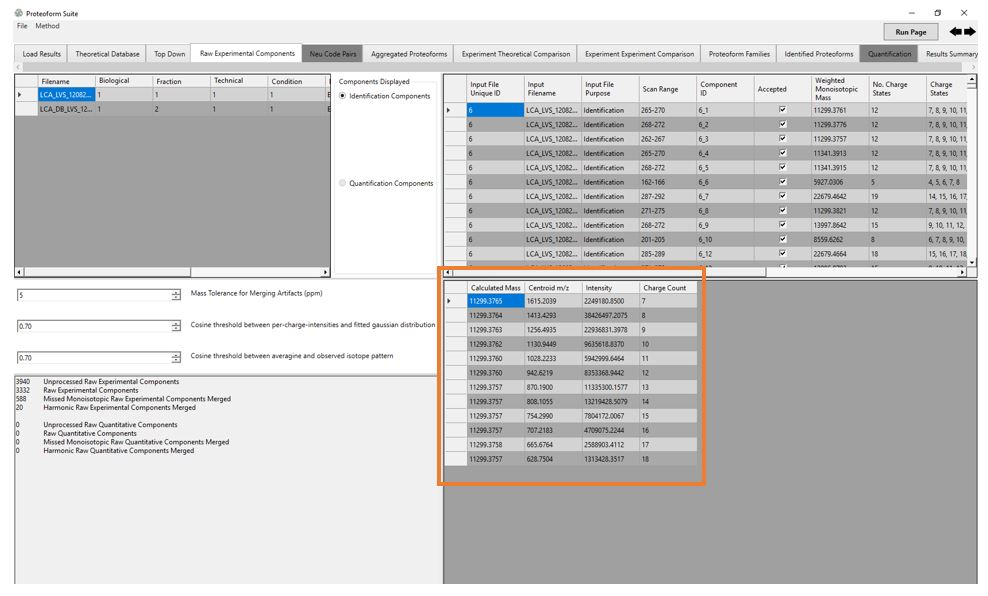
\includegraphics[scale=0.5]{figures/rawcomponents4.jpg}
\end{figure}
	\begin{itemize}
		\item Calculated Mass: monoisotopic mass of this charge state
		\item Centroid m/z: monoisotopic \textit{m/z} value of this charge state
		\item Intensity: charge normalized intensity of this charge state
		\item Charge count: number of this charge state
	\end{itemize}
\end{itemize}
\pagebreak
%!TEX root = ../proteoform_suite_manual.tex
%---------------------------------------------------------------------
%	NEUCODE PAIRS
%---------------------------------------------------------------------

\section{NeuCode Pairs}

\subsection{Overview}

On this page, NeuCode pairs are generated from the raw experimental components. Each NeuCode pair consists of a light raw experimental component and a heavy raw experimental component; the lysine count is determined based upon the delta mass difference between the light and heavy raw experimental components of the NeuCode pair. For more information on generating NeuCode labeled data for proteoform identification in Proteoform Suite, see the methods sections of previously published analyses.\supercite{Shortreed2016,Cesnik2018,Dai2017,Dai2019} 

\subsection{Run Page}
\begin{itemize}
\item The Raw Experimental Components page must be run before running this page
\item Click Run Page button (top right)
\item Set all parameters as desired for current analysis (see below). The results automatically refresh; you do not need to re-run the page after adjusting the parameters. Only accepted NeuCode pairs will be included in further analysis in Proteoform Suite.
\end{itemize}

\subsection{Set Parameters}
\begin{figure}[h]
\centering
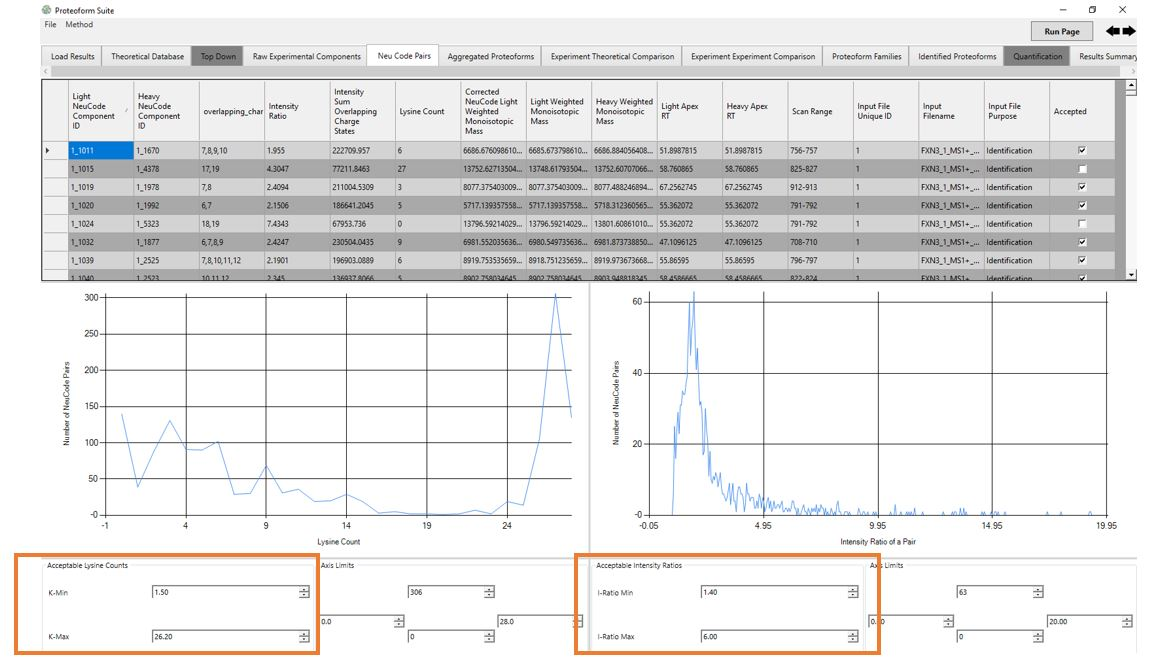
\includegraphics[scale=0.43]{figures/neucode1.jpg}
\end{figure}
\begin{itemize}
\item Acceptable Lysine Counts: only NeuCode pairs with an acceptable number of lysines will be accepted
\begin{itemize}
\item K-Min: minimum acceptable lysine count for a NeuCode pair to be accepted for further analysis
\item K-Max: maximum acceptable lysine count for a NeuCode pair to be accepted for further analysis
\end{itemize}
\item Acceptable Intensity Ratios: only NeuCode pairs with an acceptable intensity ratio between light/heavy raw experimental components will be accepted
\begin{itemize}
\item I-Ratio Min: minimum acceptable intensity ratio for a NeuCode pair to be accepted for further analysis
\item I-Ratio Max: maximum acceptable intensity ratio for a NeuCode pair to be accepted for further analysis
\end{itemize}
\end{itemize}

\subsection{Results}
\begin{itemize}
	\item NeuCode pairs table: the top table displays all NeuCode pairs generated
	\begin{figure}[h]
\centering
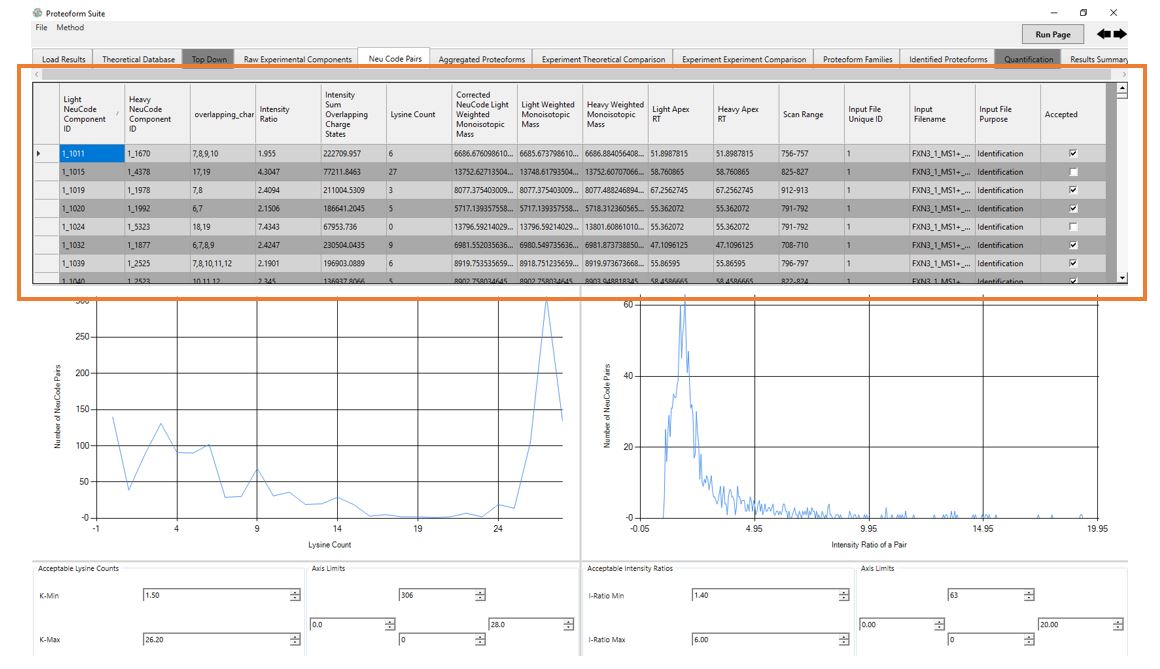
\includegraphics[scale=0.5]{figures/neucode2.jpg}
\end{figure}
\begin{itemize}
		\item Light NeuCode Component ID: Proteoform Suite given ID for the light raw experimental component; file ID\_component \#
		\item Heavy NeuCode Component ID: Proteoform Suite given ID for the heavy raw experimental component; file ID\_component \#
		\item Overlapping Charge States: comma-separated list of charge states observed for both the light and heavy raw experimental components components in this NeuCode pair
		\item Intensity Ratio: intensity ratio of light raw experimental component intensity : heavy raw experimental component intensity
		\item Intensity Sum Overlapping Charge States: summed intensity for all charge states observed for both the light and heavy raw experimental components in this NeuCode pair
		\item Lysine Count: lysine count for this NeuCode pair; determined by mass difference between light and heavy raw experimental components
		\item Corrected NeuCode Light Weighted Monoisotopic Mass: monoisotopic mass of light raw experimental component used for this NeuCode pair, monoisotopic mass errors corrected
		\item Light Weighted Monoisotopic Mass: monoisotopic mass of light raw experimental component
		\item Heavy Weighted Monoisotopic Mass: monoisotopic mass of heavy raw experimental component
		\item Light Apex RT: apex retention time of light raw experimental component
		\item Scan Range: MS scan range for light and heavy raw experimental components in this NeuCode pair
		\item Input File Unique ID: file ID number for filename of Deconvolution Results for Identification or Quantification for the light and heavy raw experimental components in this NeuCode pair
		\item Input Filename: filename of Deconvolution Results for Identification or Quantification for light and heavy raw experimental components in this NeuCode pair
		\item Input File Purpose: either Identification or Quantification
		\item Accepted: checked if this NeuCode pair has a lysine count and intensity ratio within the min and max range allowed (see Set Parameters); if accepted, this NeuCode pair will be utilized in subsequent Proteoform Suite analysis
\end{itemize}
\item Lysine Count histogram: the left graph shows a histogram of lysine counts for all NeuCode pairs. The Axis Limits box below this graph adjusts the x- and y-axes.
	\begin{figure}[h]
\centering
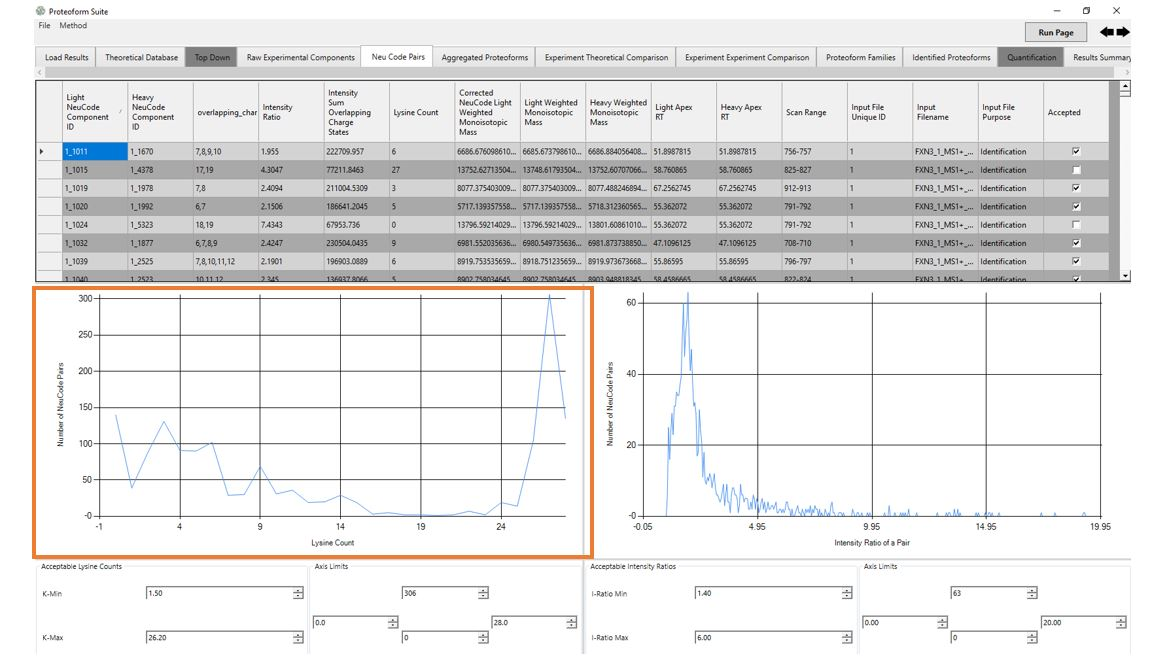
\includegraphics[scale=0.5]{figures/neucode3.jpg}
\end{figure}
\pagebreak
\item Intensity Ratio histogram: the right graph shows a histogram of light:heavy intensity ratios for all NeuCode pairs. The peak of this histogram should fall close to the experimentally performed mixing ratio for light:heavy protein samples (ex: 2:1 light:heavy). The Axis Limits box below this graph adjusts the x- and y-axes.
	\begin{figure}[h]
\centering
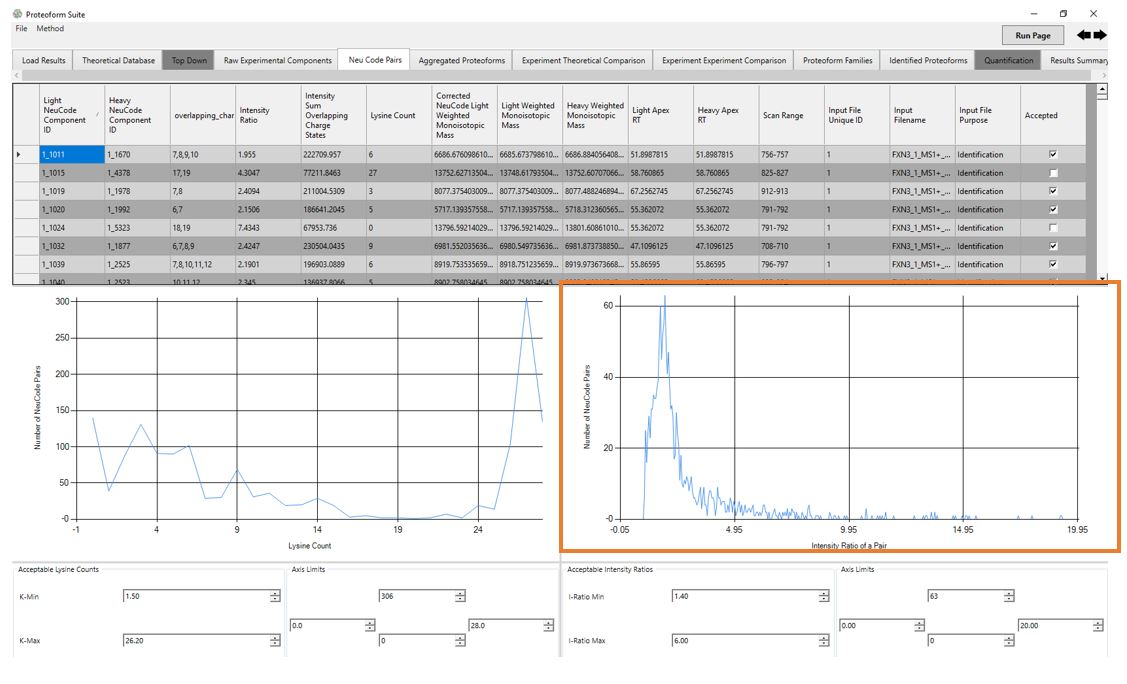
\includegraphics[scale=0.5]{figures/neucode4.jpg}
\end{figure}
\end{itemize}
\pagebreak
%!TEX root = ../proteoform_suite_manual.tex
%---------------------------------------------------------------------
%	AGGREGATED PROTEOFORMS
%---------------------------------------------------------------------

\section{Aggregated Proteoforms}

\subsection{Overview}

On this page, experimental proteoforms are created by aggregating either raw experimental components (unlabeled analysis) or NeuCode pairs (NeuCode labeled analysis). If Deconvolution Results for Quantification were provided on the Load Results page, these raw experimental components for quantification will be binned with experimental proteoforms based upon the set parameters. The experimental proteoforms are used in intact-mass analysis to identify proteoforms and construct proteoform families.

\subsection{Run Page}
\begin{itemize}
\item The Raw Experimental Components page must be run before running this page. If applicable, the Top-Down and the NeuCode Pairs pages must also be run before running this page.
\item Set all parameters as desired for current analysis (see below)
\item Click Run Page button (top right)
\end{itemize}

\subsection{Set Parameters}
\begin{figure}[h]
\centering
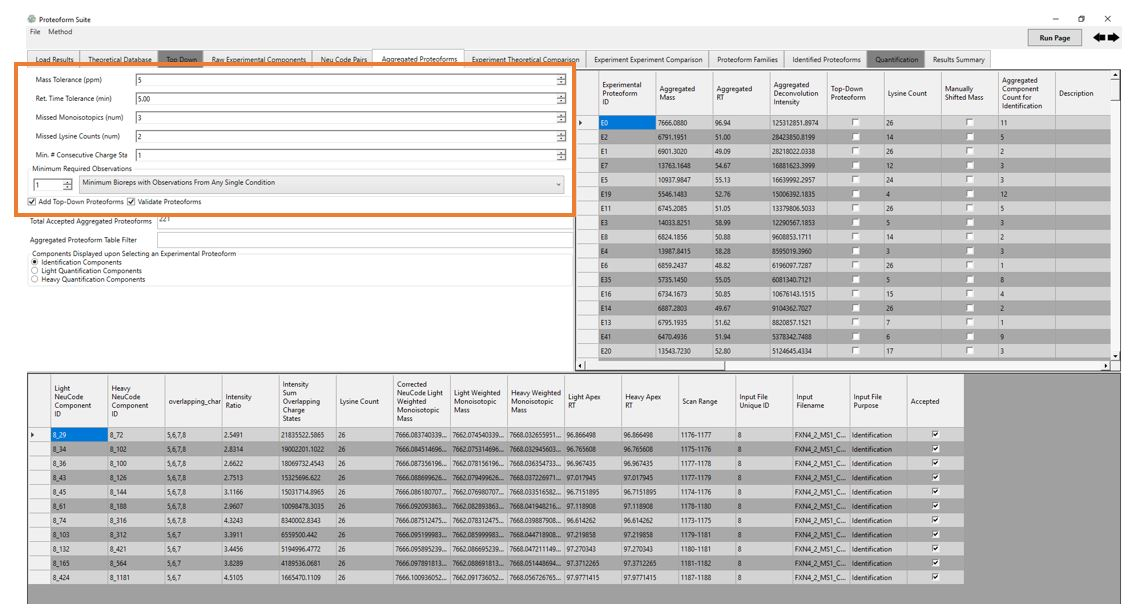
\includegraphics[scale=0.5]{figures/aggregated_proteoforms1.jpg}
\end{figure}
\begin{itemize}
\item Mass Tolerance (ppm): mass tolerance used to aggregate raw experimental components (unlabeled) or NeuCode pairs (NeuCode labeled)
\item Ret. Time Tolerance (min): retention time tolerance used to aggregate raw experimental components (unlabeled) or NeuCode pairs (NeuCode labeled)
\item Missed Monoisotopics (num): number of missed monoisotopic units to aggregate raw experimental components (unlabeled) or NeuCode pairs (NeuCode labeled)
\item Missed Lysine Counts (num): the number of missed lysine counts to aggregate NeuCode pairs (accounts for <100\% labeling efficiency)
\item Min. \# Consecutive Charge States:  minimum number of charge states for a raw experimental component to be considered for aggregation
\item Minimum Required Observations: set the \# (left) and the requirement (right drop down box) to require observations of an experimental proteoform in more than one file type. Must have labeled biological replicates, technical replicates, and conditions for Deconvolution Results for Identification on the Load Results page
\item Add Top-Down Proteoforms: if checked, top-down proteoforms from the Top Down page will be aggregated with experimental proteoforms created from raw experimental components (unlabeled) or NeuCode pairs (NeuCode labeled). Top-down proteoforms will replace experimental proteoforms using the set parameters above
\item Validate Proteoforms: if checked and if NeuCode labeled data, will verify that aggregated NeuCode pairs are in the tolerances determined with set parameters
\end{itemize}

\subsection{Results}
\begin{itemize}
	\item Total Accepted Aggregated Proteoforms: the number of accepted experimental proteoforms that will be included in further analysis
	\item Aggregated Proteoform Table Filter: filter the Aggregated Proteoforms table (top right) by any entered text
	\item Components Displayed Upon Selecting an Experimental Proteoform: determines which components will be displayed in the Components table (bottom) when an aggregated proteoform is selected in the Aggregated Proteoform Table (right)
	\begin{figure}[h]
\centering
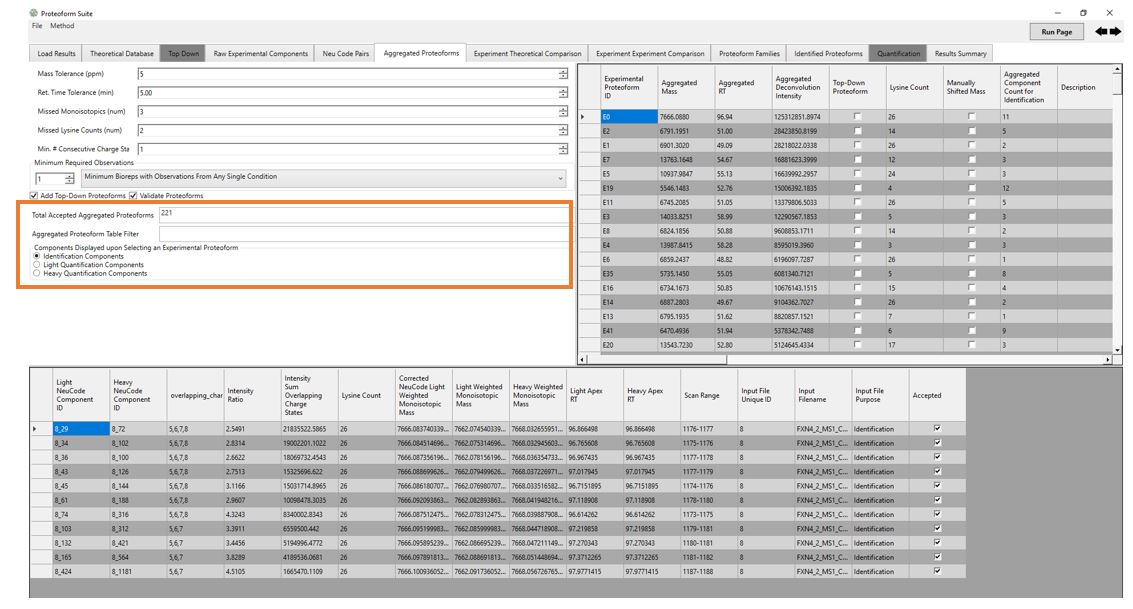
\includegraphics[scale=0.5]{figures/aggregated_proteoforms2.jpg}
\end{figure}
\pagebreak
	\item Aggregated Proteoforms table: the top right table displays the aggregated experimental proteoforms
		\begin{figure}[h]
\centering
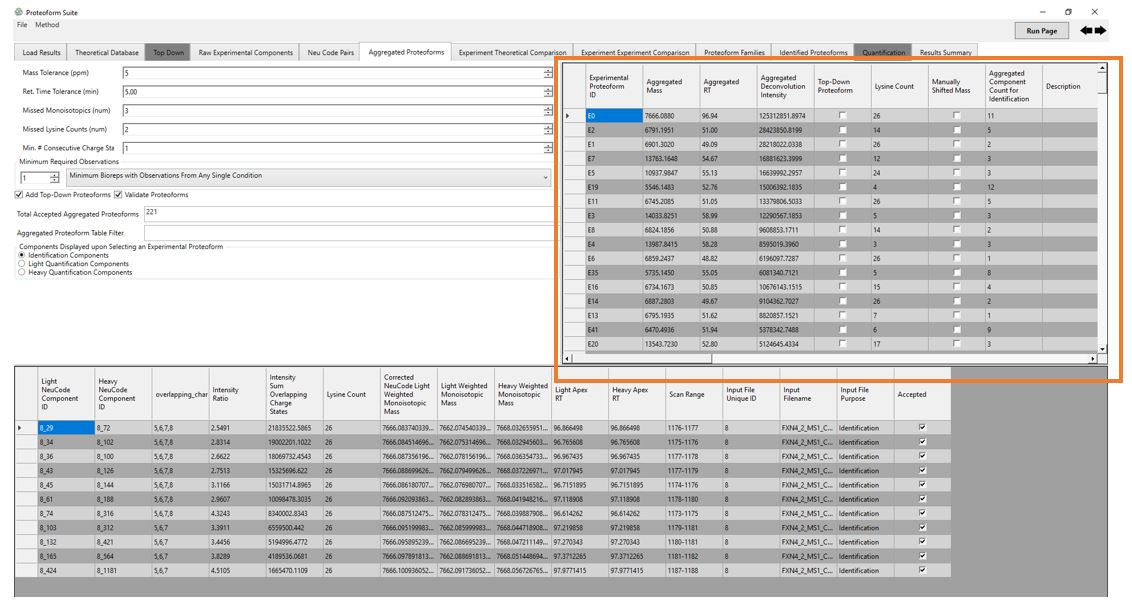
\includegraphics[scale=0.5]{figures/aggregated_proteoforms3.jpg}
\end{figure}
	\begin{itemize}
		\item Experimental Proteoform ID: unique ID given by Proteoform Suite for this experimental proteoform
		\item Aggregated Mass: monoisotopic mass of experimental proteoform, weighted average of (light) raw experimental components by intensity
		\item Aggregated RT: retention time of experimental proteoform, average of raw experimental components (unlabeled) or NeuCode pairs (NeuCode labeled)
		\item Aggregated Deconvolution Intensity: sum of intensity of aggregated raw experimental components
		\item Top-Down Proteoform: checked if this experimental proteoform is a top-down identified proteoform
		\item Lysine Count: number of lysines (NeuCode labeled data)
		\item Manually Shifted Mass: checked if monoisotopic mass was shifted by an isotopic mass unit (see \textbf{Experiment-Theoretical Comparison} section)
		\item Aggregated Component Count for Identification: number of aggregated raw experimental components (unlabeled) or NeuCode pairs (NeuCode labeled). If top-down proteoform, the number of top-down hits
		\item Description: if identified, the protein description from UniProt
		\item Gene Name: if identified, the gene name
		\item GeneID: if identified, the gene ID
		\item Grouped Accessions: if identified, the protein accessions from UniProt
		\item PTM Description: if identified, the post-translational modifications on this experimental proteoform
		\item Begin and End: if identified, the experimental proteoform begin and end residue in protein full sequence in UniProt
		\item Sequence: if identified, proteoform sequence
		\item UniProt-Annotated Modifications: if identified, all UniProt annotated residues for PTMs on this experimental  proteoform in UniProt database provided
		\item Potentially Novel Mods: if identified, checked if this experimental proteoform contains PTMs not annotated in UniProt database provided	
		\item Bottom-Up PSMs Count: if identified, the number of bottom-up PSMs derived from this experimental proteoform
		\item Modified Bottom-Up PSMs: if identified, modified residues confirmed by ID'd bottom-up peptides derived from this experimental proteoform
		\item Bottom-Up Evidence for All PTMs: if identified, checked if all PTMs on this experimental		
		\item Level: proteoform identification level based on five-level scheme\supercite{Smith2019b}
		\item Level Description: description of proteoform level assignment (sources of ambiguity)
		\item New Intact-Mass ID: if identified, this intact-mass identification was not identified by top-down
		\item Ambiguous: checked if ambiguous intact-mass identification
		\item Adduct: checked if identification is due to presence of an adduct (oxidation, SDS adduct, sulfate adduct)
		\item Contaminant: checked if identification is from a theoretical proteoform in a contaminant database
		\item Mass Error: mass difference between observed mass and theoretical mass of this identification
		\item Family ID: proteoform family number (must have run through full Proteoform Suite analysis)
		\item Family: identified, ambiguous, or unidentified proteoform family
		\item Linked Proteoform References: proteoforms in family network path of identification to the nearest theoretical proteoform (must have run through full Proteoform Suite analysis)
		\item M/z values: m/z values observed for this experimental proteoform
		\item Charges: charge state numbers observed for this experimental proteoform
		\item Abundant Component for Manual Validation of Identification: file information for the most abundant raw experimental component aggregated into this experimental proteoform
	\end{itemize}
	\item Components table: the bottom table displays all raw experimental components (unlabeled) or NeuCode pairs (NeuCode labeled) aggregated into the experimental proteoform selected in the Aggregated Proteoforms table (top right)
		\begin{figure}[h]
\centering
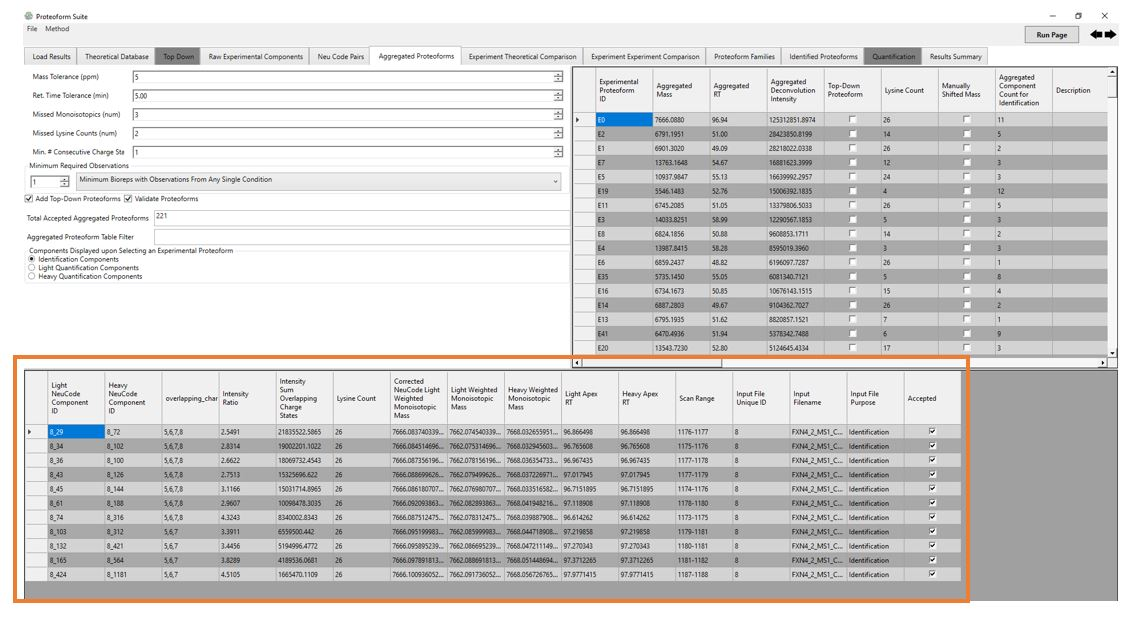
\includegraphics[scale=0.5]{figures/aggregated_proteoforms4.jpg}
\end{figure}
	\begin{itemize}
		\item See Raw Experimental Components table in \textbf{Raw Experimental Components} section (unlabeled) or NeuCode Pairs table in \textbf{NeuCode Pairs} section (NeuCode labeled) for a description of each column
	\end{itemize}
\end{itemize}
\pagebreak
%!TEX root = ../proteoform_suite_manual.tex
%---------------------------------------------------------------------
%	EXPERIMENT THEORETICAL COMPARISON
%---------------------------------------------------------------------

\section{Experiment Theoretical Comparison}

\subsection{Overview}

On this page, experimental proteoforms are compared to theoretical proteoforms from the theoretical database, generating a list of experiment-theoretical pairs. Each experiment-theoretical pair has a mass difference between the experimental proteoform and the theoretical proteoform in the pair; pairs are generated for mass differences that correspond to a known set of modifications. Each experimental proteoform can be in a pair with one theoretical proteoform per protein; heuristics are used to determine the most likely pair based on the delta mass differences. A histogram is generated of the mass differences for all experiment-theoretical pairs; experiment-theoretical pairs in accepted delta mass peaks are used to construct proteoform families. Experiment-decoy pairs are generated by comparing the experimental proteoforms to the decoy databases; these pairs are used to estimate a false discovery rate for each delta mass peak. 

\subsection{Run Page}
\begin{itemize}
\item The Theoretical Proteoforms and Aggregated Proteoforms pages must be run before running this page.
\item Set all parameters as desired for current analysis (see below)
\item Click Run Page button (top right)
\item Browse the list of delta mass peaks from the histogram of experimental-theoretical pairs delta masses (top left table). Accept peaks that have an acceptable false discovery rate and correspond to common/likely modifications. For unlabeled analyses, typically only the delta mass peak closest to 0 (exact matches) is accepted. 
\end{itemize}

\subsection{Set Parameters}
\begin{figure}[h]
\centering
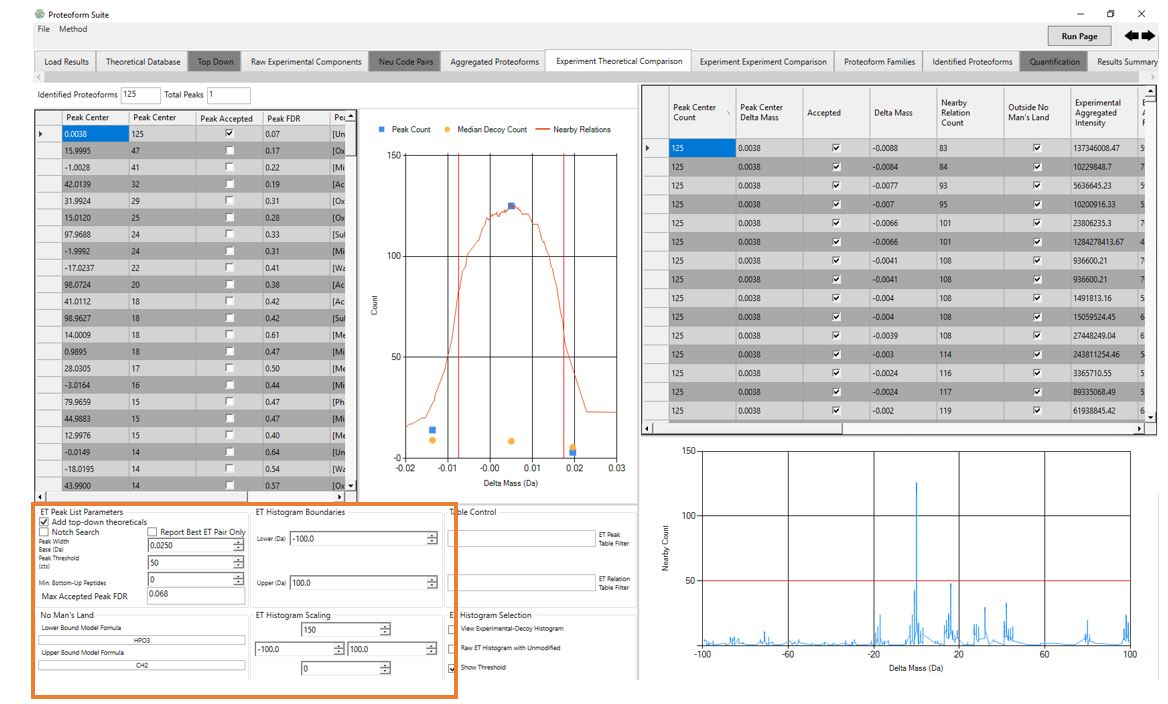
\includegraphics[scale=0.43]{figures/et1.jpg}
\end{figure}
\begin{itemize}
\item Add top-down theoreticals: if checked, theoretical proteoforms that were supplemented to the database due to the presence of a top-down proteoforms will be included in the experiment-theoretical comparison
\item Notch Search: if checked, a notch search will be performed. For each modification, experiment-theoretical pairs will be generated if the delta mass is within the set tolerance from the modification's delta mass
\item Report Best ET Pair Only: if checked, only the closest matching experiment-theoretical pair for each experimental proteoform will be included (each experimental proteoform will only be able to belong to one experiment-theoretical pair)
\item Peak Width Base (Da): if notch search is unchecked, this is the size of bins used for generating the delta mass histogram from experiment-theoretical pair delta masses
\item Peak Threshold (cts): the minimum number of experiment-theoretical pairs that must belong to a delta mass peak for the peak to be accepted
\item Min. Bottom-Up Peptides: this is the minimum number of bottom-up peptides that a theoretical proteoform must have in order to be included in the experiment-theoretical comparison
\item Notch Tolerance: if a notch search is performed, this tolerance will be used to generate experiment-theoretical pairs at each modification delta mass
\item ET Histogram Boundaries: Lower (Da) and Upper (Da) delta masses to be considered for an experiment-theoretical pair to be generated 
\end{itemize}

\subsection{Results}
\begin{itemize}
	\item Identified Proteoforms: the number of accepted experimental-theoretical pairs
	\item Total Peaks: the number of accepted experiment-theoretical delta mass peaks
	\pagebreak
	\item Experimental-Theoretical Delta Mass Peaks table: the top left table displays the delta mass peaks from the histogram of experiment-theoretical pair delta masses. If a notch search is performed, each peak is a different modification delta mass/notch

	\begin{figure}[h]
\centering
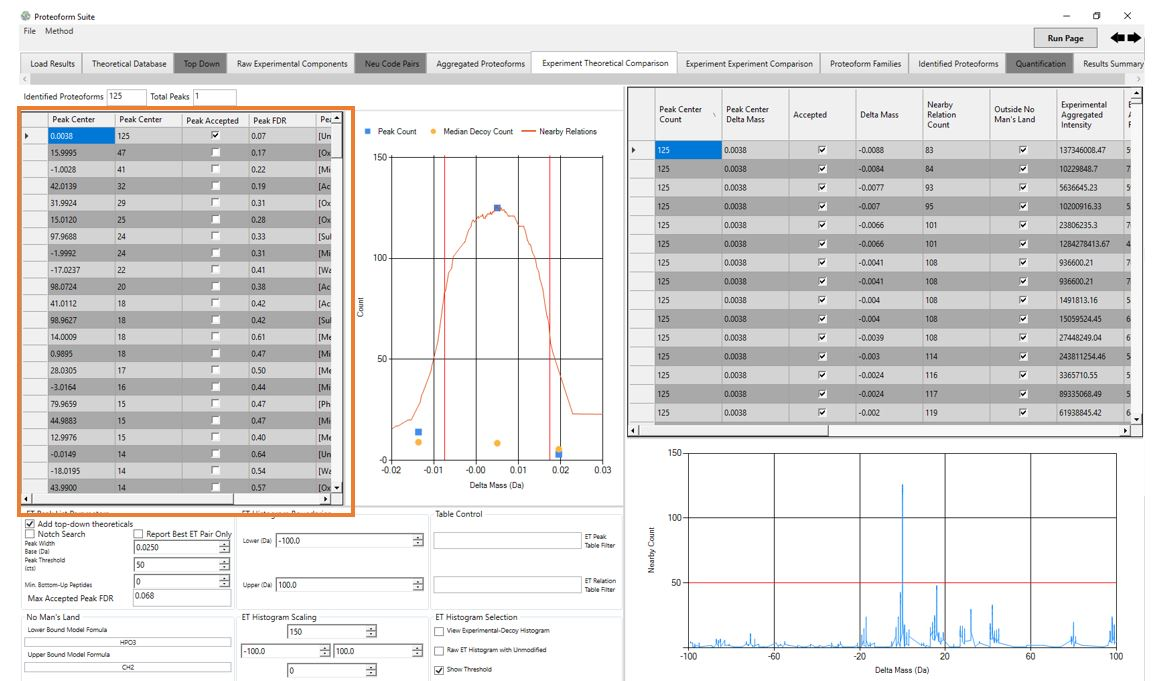
\includegraphics[scale=0.46]{figures/et2.jpg}
\end{figure}
	\begin{itemize}
		\item Peak Center Delta Mass: delta mass at the center of this delta mass peak 
		\item Peak Center Count: the number of experiment-theoretical comparisons delta masses that are part of this peak
		\item Peak Accepted: checked if peak is accepted (peak center count is above peak threshold in set parameters or manually changed by user). This check box can be checked or unchecked to accept or unaccept a delta mass peak
		\item Peak FDR: the false discovery rate for this delta mass peak; determined based on the average number of experiment-decoy pairs that fall within this peak delta mass plus/minus half of the peak width base
		\item Peak Assignment Possibilities: modifications/combinations of modifications that could correspond to the delta mass of this delta mass peak
		\item Mass Shifter: set this number to a positive or negative integer and rerun this page; the monoisotopic mass of experimental proteoforms in experiment-theoretical pairs in this peak will be shifted by the number of monoisotopic mass units of this column; useful if a peak is at a missed monoisotopic value from 0 or a modification delta mass (ex: -1 or +1 Da)
	\end{itemize}
	\item Experiment-Theoretical Delta Mass Peak Zoom-in Graph: when a peak is selected in the Experiment-Theoretical Delta Mass Peak table, this top left graph displays a zoom-in of the peak from the Experiment-Theoretical Delta Mass Histogram (bottom right graph). Blue square point is the number of experiment-theoretical pairs in the peak, and yellow circle point is median number of experiment-decoy pairs in this peak. The red line plots the nearby relations histogram count for each delta mass value
		\begin{figure}[h]
\centering
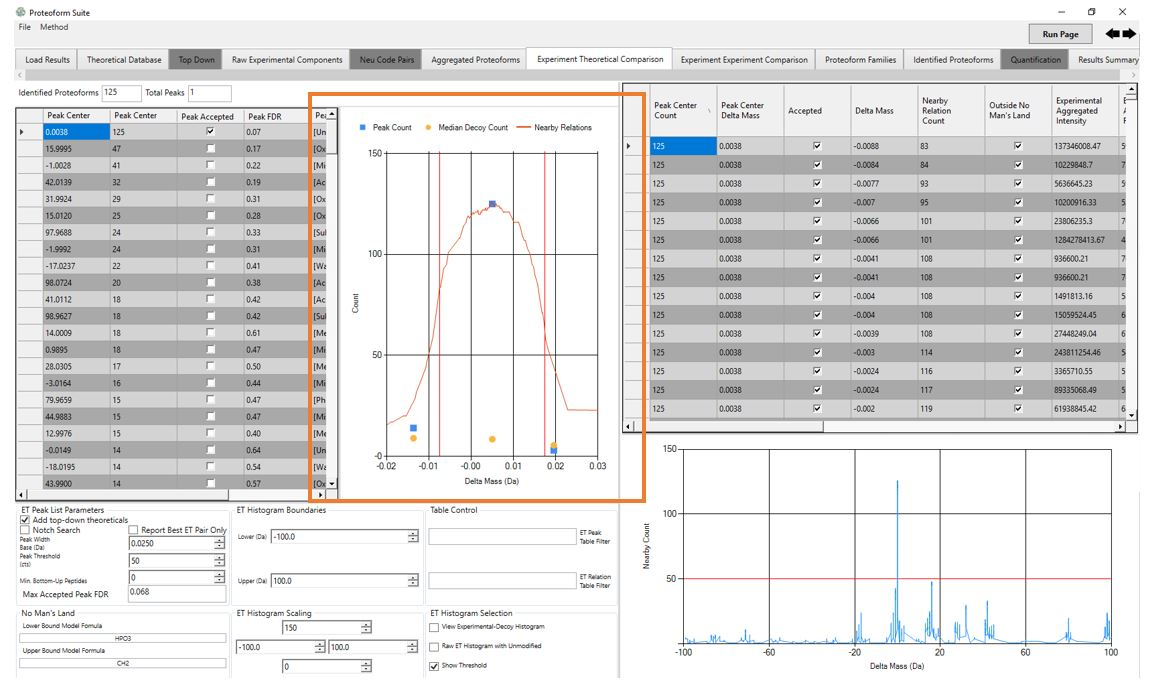
\includegraphics[scale=0.44]{figures/et3.jpg}
\end{figure}
\item {Experiment-Theoretical Pairs}: this right table displays all experiment-theoretical pairs, consisting of a theoretical proteoform, an experimental proteoform, and their mass difference.
		\begin{figure}[h]
\centering
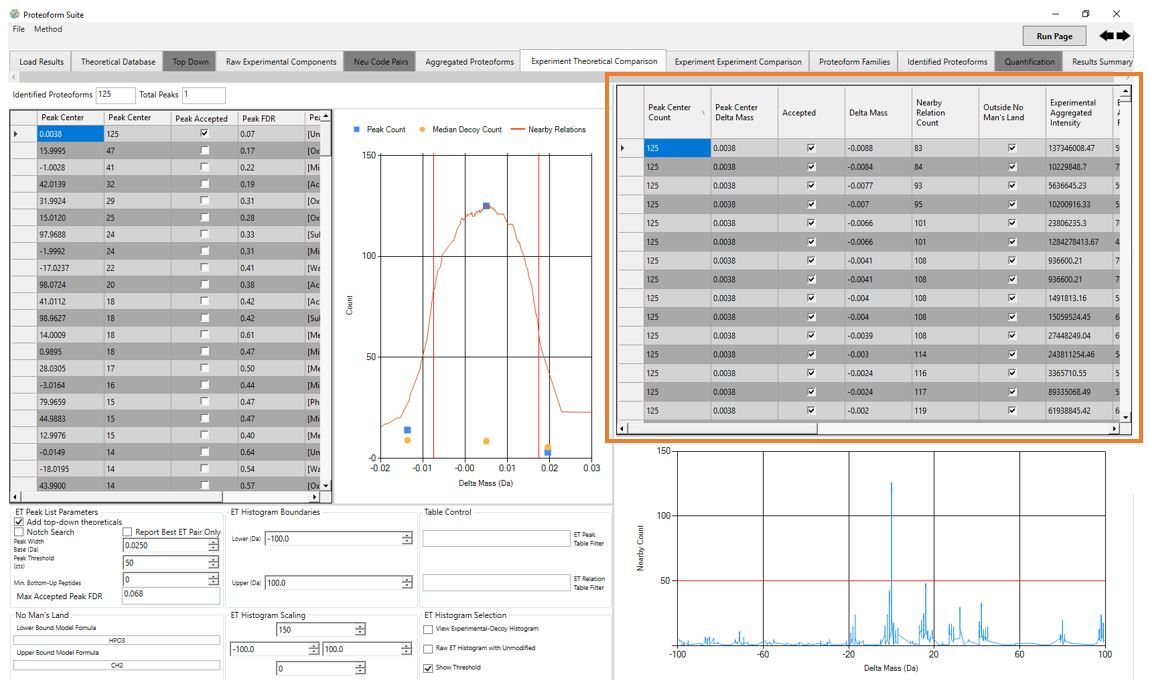
\includegraphics[scale=0.44]{figures/et4.jpg}
\end{figure}
\begin{itemize}
	\item Peak Center Count: if this pair is in a delta mass peak, the number of pairs in the peak
	\item Peak Center Delta Mass: if this pair is in a delta mass peak, the delta mass at the center of the peak
	\item Accepted: checked if this pair is in a delta mass peak that is accepted in the Experimental-Theoretical Delta Mass Peaks table
	\item Delta Mass: mass difference between the experimental and theoretical proteoform in this pair
	\item Nearby Relation Count: number of pairs with a delta mass close to this pair's delta mass; this value is used to plot the delta mass histogram
	\item Outside No Man's Land: checked if this pair is an acceptable delta mass regarding the numbers after the decimal point. Pairs with a delta mass in no man's land are not joined into delta mass peaks
	\item Experimental Aggregated Intensity: sum of intensity of aggregated raw experimental components for the experimental proteoform in this pair
	\item Experimental Aggregated RT: retention time of experimental proteoform in this pair
	\item Number Experimental Observations: number of aggregated raw experimental components (unlabeled) or NeuCode pairs (NeuCode labeled) for the experimental proteoform in this pair. If top-down proteoform, the number of top-down hits
	\item Experimental Aggregated Proteoform Mass: mass of experimental proteoform in this pair
	\item Experimental Accession: unique ID given by Proteoform Suite for experimental proteoform in this pair		
	\item Abundant Exp. Component for Manual Validation: file information for the most abundant raw experimental component aggregated into the experimental proteoform of this pair
	\item Theoretical Proteoform Mass: mass of theoretical proteoform in this pair
	\item Accession: accession given by Proteoform Suite for the theoretical proteoform in this pair
	\item Name: protein name from UniProt for the theoretical proteoform in this pair
	\item Fragment: sequence description for the theoretical proteoform in this pair
	\item Description: protein description from UniProt for the theoretical proteoform in this pair
	\item PTM Description: PTMs on theoretical proteoform in this pair
\end{itemize}
\pagebreak
\item Experiment-Theoretical Delta Mass Histogram graph: this bottom right graph shows a histogram of the delta masses for the experiment-theoretical pairs
\begin{figure}[h]
\centering
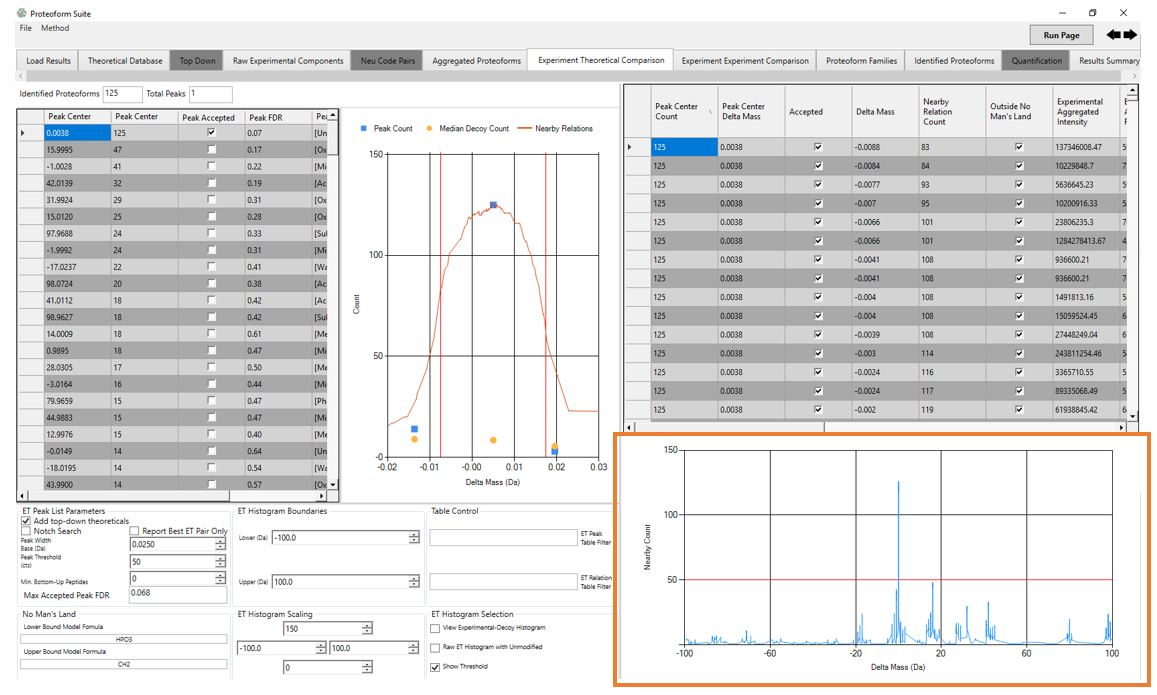
\includegraphics[scale=0.46]{figures/et5.jpg}
\end{figure}
\begin{itemize} 
	\item View Experiment Decoy Histogram: if checked, delta mass histogram for experiment decoy pairs will be plotted
	\item Raw ET Histogram with Unmodified: if checked, a histogram with only unmodified theoretical proteoforms will be plotted using all delta mass pairs
	\item Show Threshold: if checked, a red line on the graph shows the Peak Threshold set
	\end{itemize}
\end{itemize}
\pagebreak
%!TEX root = ../proteoform_suite_manual.tex
%---------------------------------------------------------------------
%	EXPERIMENT Theoretical	EXPERIMENT COMPARISON
%---------------------------------------------------------------------

\section{Experiment Experiment Comparison}

\subsection{Overview}

On this page, experimental proteoforms are compared to one another, generating a list of experiment-experiment pairs. Each experiment-experiment pair has a mass difference between the two experimental proteoforms in the pair. A histogram is generated of the mass differences for all experiment-experiment pairs; experiment-experiment pairs in accepted delta mass peaks are used to construct proteoform families. Experiment-false pairs are generated from experimental proteoforms with a different number of lysines (NeuCode labeled) or from proteoforms eluting at a different retention times (unlabeled); these pairs are used to estimate a false discovery rate for each delta mass peak. 

\subsection{Run Page}
\begin{itemize}
\item The Theoretical Proteoforms and Aggregated Proteoforms pages must be run before running this page.
\item Set all parameters as desired for current analysis (see below)
\item Click Run Page button (top right)
\item Browse the list of delta mass peaks from the histogram of experimental-theoretical pairs delta masses (top left table). Accept peaks that have an acceptable false discovery rate and correspond to common/likely modifications. 
\end{itemize}

\subsection{Set Parameters}
\begin{figure}[h]
\centering
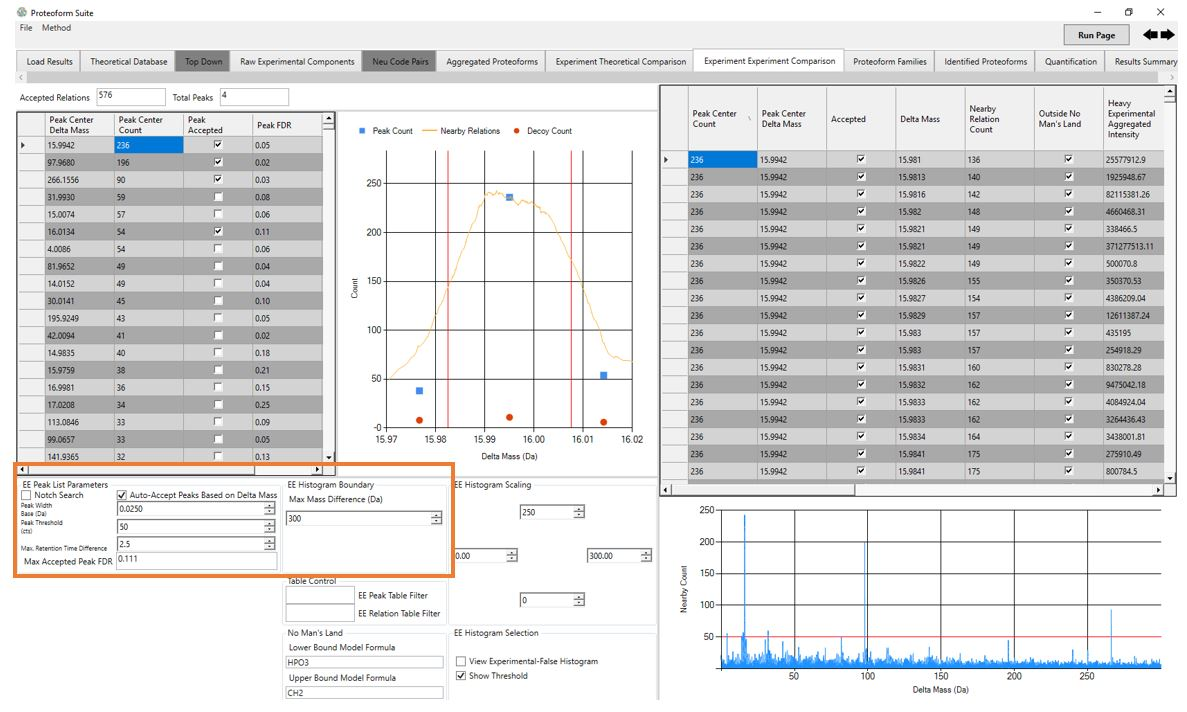
\includegraphics[scale=0.43]{figures/ee1.jpg}
\end{figure}
\begin{itemize}
\item Notch Search: if checked, a notch search will be performed. For each modification, experiment-experiment pairs will be generated if the delta mass is within the set tolerance from the modification's delta mass
\item Auto-Accept Peaks Based on Delta Mass: if checked, peaks with a count above the Peak Threshold will be accepted if they correspond to a common modification
\item Peak Width Base (Da): if notch search is unchecked, this is the size of bins used for generating the delta mass histogram from experiment-experiment pair delta masses
\item Peak Threshold (cts): the minimum number of experiment-experiment pairs that must belong to a delta mass peak for the peak to be accepted
\item Max. Retention Time Difference: maximum allowed retention time difference for two experimental proteoforms to be eligible to be in an experiment-experiment pair
\item Notch Tolerance: if a notch search is performed, this tolerance will be used to generate experiment-experiment pairs at each modification delta mass
\item EE Histogram Boundary: maximum delta masses to be considered for an experiment-theoretical pair to be generated 
\end{itemize}

\subsection{Results}
\begin{itemize}
	\item Accepted Relations: the number of accepted experimental-experiment pairs
	\item Total Peaks: the number of accepted experiment-experiment delta mass peaks
	\item Experimental-Experiment Delta Mass Peaks table: the top left table displays the delta mass peaks from the histogram of experiment-experiment pair delta masses. If a notch search is performed, each peak is a different modification delta mass/notch
	\begin{figure}[h]
\centering
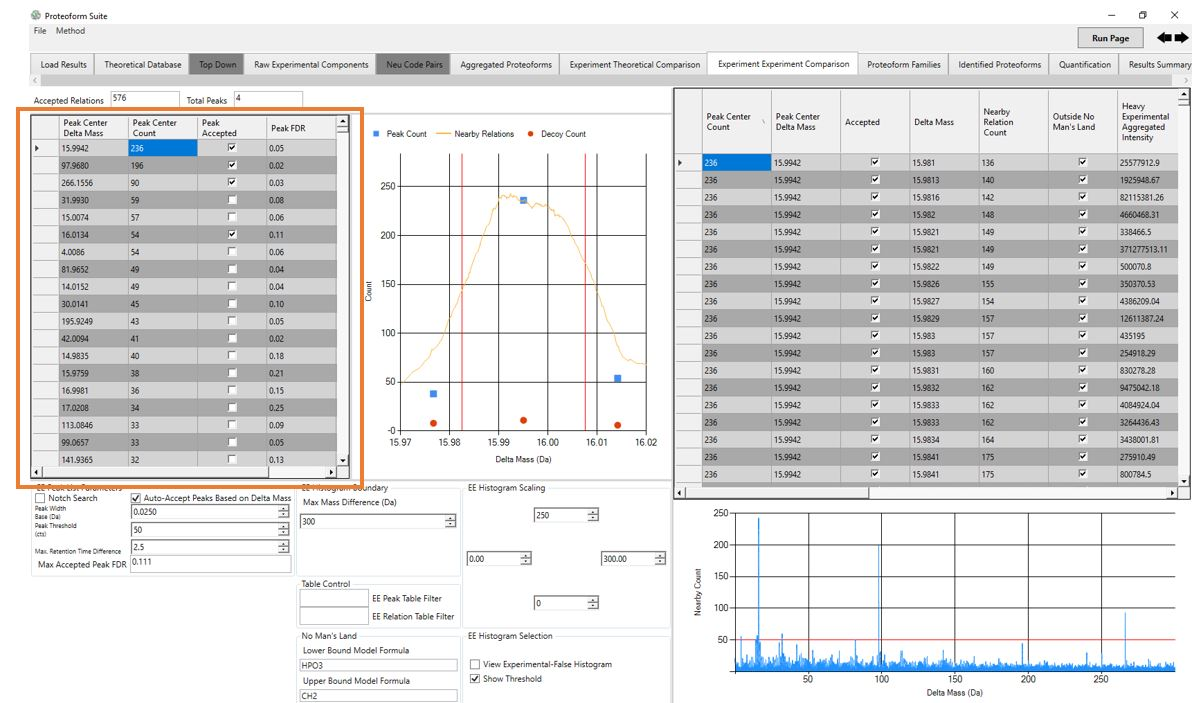
\includegraphics[scale=0.43]{figures/ee2.jpg}
\end{figure}
	\begin{itemize}
		\item Peak Center Delta Mass: delta mass at the center of this delta mass peak 
		\item Peak Center Count: the number of experiment-experiment comparisons delta masses that are part of this peak
		\item Peak Accepted: checked if peak is accepted (peak center count is above peak threshold in set parameters or manually changed by user). This check box can be checked or unchecked to accept or unaccept a delta mass peak
		\item Peak FDR: the false discovery rate for this delta mass peak; determined based on the number of experiment-false pairs that fall within this peak delta mass plus/minus half of the peak width base
		\item Peak Assignment Possibilities: modifications/combinations of modifications that could correspond to the delta mass of this delta mass peak
		\end{itemize}
	\item Experiment-Experiment Delta Mass Peak Zoom-in Graph: when a peak is selected in the Experiment-Experiment Delta Mass Peak table, this top left graph displays a zoom-in of the peak from the Experiment-Experiment Delta Mass Histogram (bottom right graph). Blue square point is peak count, and yellow circle point is median decoy count for this peak. The red line plots the nearby relations histogram count for each delta mass value
		\begin{figure}[h]
\centering
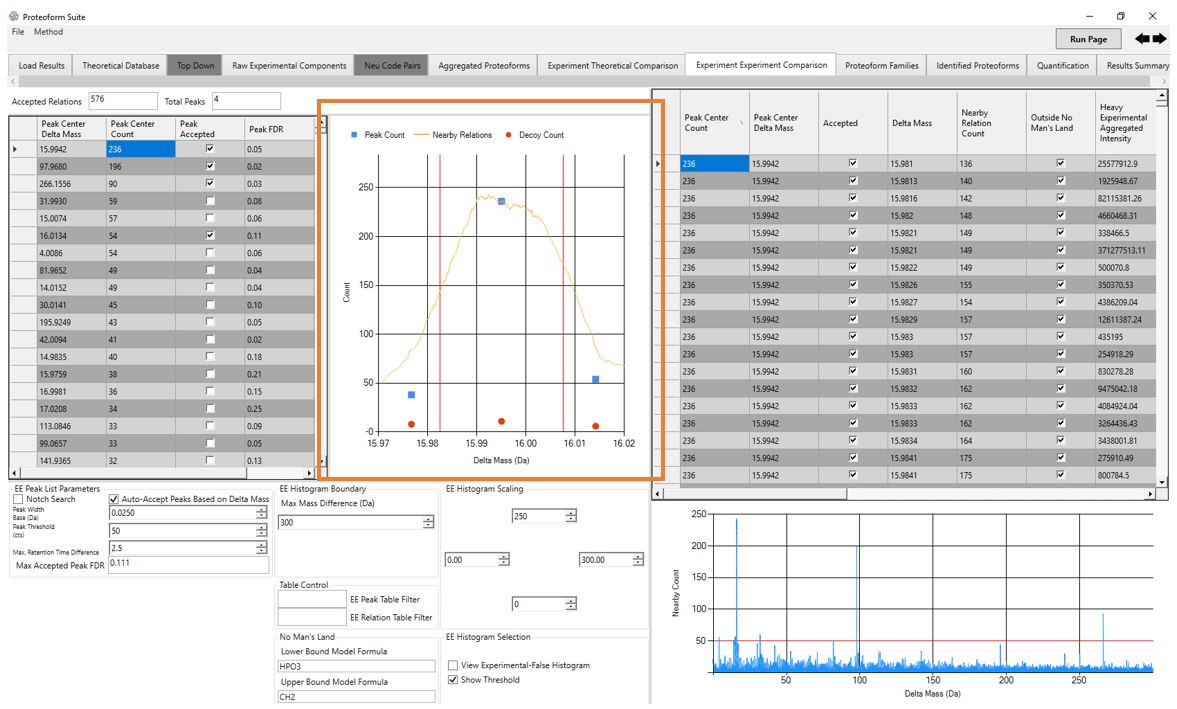
\includegraphics[scale=0.44]{figures/ee3.jpg}
\end{figure}
\pagebreak
\item {Experiment-Experiment Pairs}: this right table displays all experiment-experiment pairs, consisting of two experimental proteoforms and their mass difference.
		\begin{figure}[h]
\centering
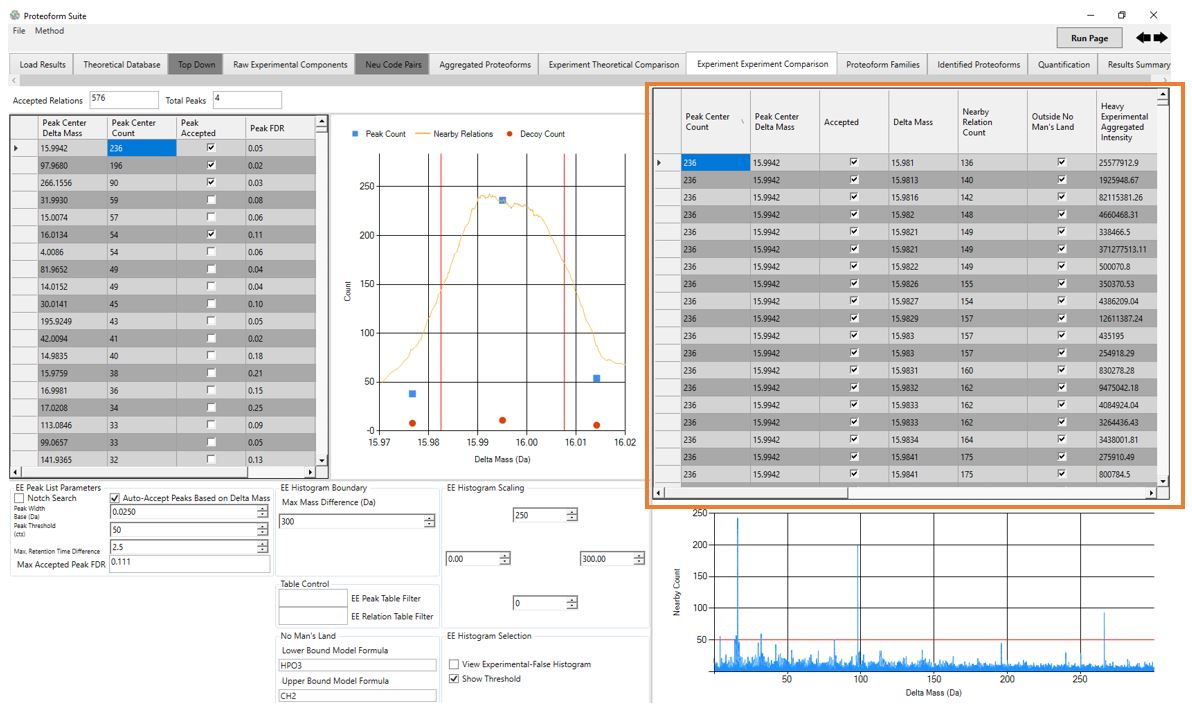
\includegraphics[scale=0.44]{figures/ee4.jpg}
\end{figure}
\begin{itemize}
	\item Peak Center Count: if this pair is in a delta mass peak, the number of pairs in the peak
	\item Peak Center Delta Mass: if this pair is in a delta mass peak, the delta mass at the center of the peak
	\item Accepted: checked if this pair is in a delta mass peak that is accepted in the Experimental-Experiment Delta Mass Peaks table
	\item Delta Mass: mass difference between the two experimental proteoforms in this pair
	\item Nearby Relation Count: number of pairs with a delta mass close to this pair's delta mass; this value is used to plot the delta mass histogram
	\item Outside No Man's Land: checked if this pair is an acceptable delta mass regarding the numbers after the decimal point. Pairs with a delta mass in no man's land are not joined into delta mass peaks
	\item Heavy Experimental Aggregated Intensity: sum of intensity of aggregated raw experimental components for the heavier experimental proteoform in this pair
	\item Aggregated RT Heavy: retention time of heavier experimental proteoform in this pair
	\item Number Heavy Experimental Observations: number of aggregated raw experimental components (unlabeled) or NeuCode pairs (NeuCode labeled) for the heavier experimental proteoform in this pair. If top-down proteoform, the number of top-down hits
	\item Heavy Experimental Aggregated Proteoform Mass: mass of the heavier experimental proteoform in this pair
	\item Heavy Experimental Accession: unique ID given by Proteoform Suite for the heavier experimental proteoform in this pair		
	\item Heavy Abundant Exp. Component for Manual Validation: file information for the most abundant raw experimental component aggregated into the heavier experimental proteoform of this pair
	\item Light Experimental Aggregated Intensity: sum of intensity of aggregated raw experimental components for the lighter experimental proteoform in this pair
	\item Aggregated RT Light: retention time of lighter experimental proteoform in this pair
	\item Number Light Experimental Observations: number of aggregated raw experimental components (unlabeled) or NeuCode pairs (NeuCode labeled) for the lighter experimental proteoform in this pair. If top-down proteoform, the number of top-down hits
	\item Light Experimental Aggregated Proteoform Mass: mass of the lighter experimental proteoform in this pair
	\item Light Experimental Accession: unique ID given by Proteoform Suite for the lighter experimental proteoform in this pair		
	\item Light Abundant Exp. Component for Manual Validation: file information for the most abundant raw experimental component aggregated into the lighter experimental proteoform of this pair
\end{itemize}
\item Experiment-Experiment Delta Mass Histogram graph: this bottom right graph shows a histogram of the delta masses for the experiment-theoretical pairs
\begin{figure}[h]
\centering
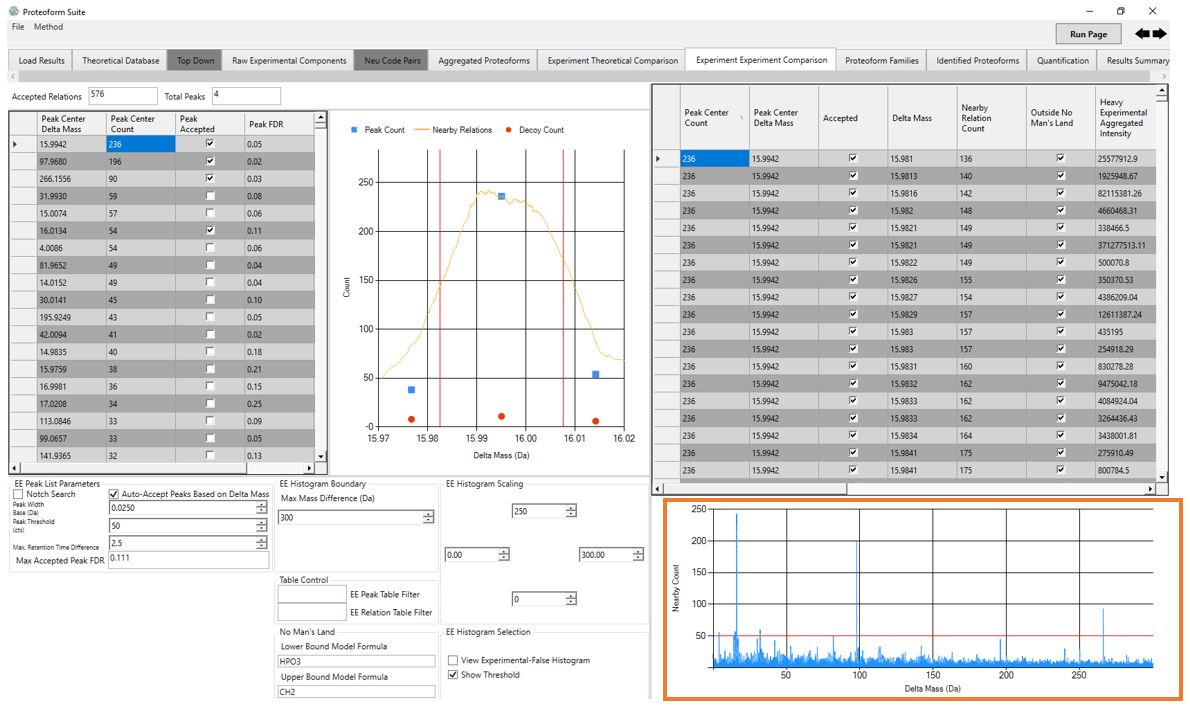
\includegraphics[scale=0.46]{figures/ee5.jpg}
\end{figure}
\begin{itemize} 
	\item View Experiment False Histogram: if checked, delta mass histogram for experiment false pairs will be plotted
	\item Show Threshold: if checked, a red line on the graph shows the Peak Threshold set
	\end{itemize}
\end{itemize}
\pagebreak
%!TEX root = ../proteoform_suite_manual.tex
%---------------------------------------------------------------------
%	PROTEOFORM FAMILIES
%---------------------------------------------------------------------

\section{Proteoform Families}

\subsection{Overview}

On this page, accepted experiment-theoretical and experiment-experiment pairs are joined to construct proteoform families. Experimental proteoforms are identified by intact-mass analysis; beginning with each theoretical proteoform in each family, connections between proteoforms are traced to identify proteoforms first from experiment-theoretical pairs and then from subsequent experiment-experiment pairs. Decoy proteoform families are constructed from experiment-decoy and experiment-false pairs and are used to calculate a global false discovery rate for intact-mass proteoform identifications. A script for Cytoscape\supercite{Shannon2003,Smoot2011} can be exported to visualize proteoform families as a network of nodes (proteoforms masses) and edges (mass differences between proteoforms). 

\subsection{Run Page}
\begin{itemize}
\item The Experiment-Theoretical Comparison and Experiment-Experiment Comparison pages must be run before running this page.
\item Set all parameters as desired for current analysis (see below)
\item Click Run Page button (top right)
\end{itemize}

\subsection{Set Parameters}
\begin{figure}[h]
\centering
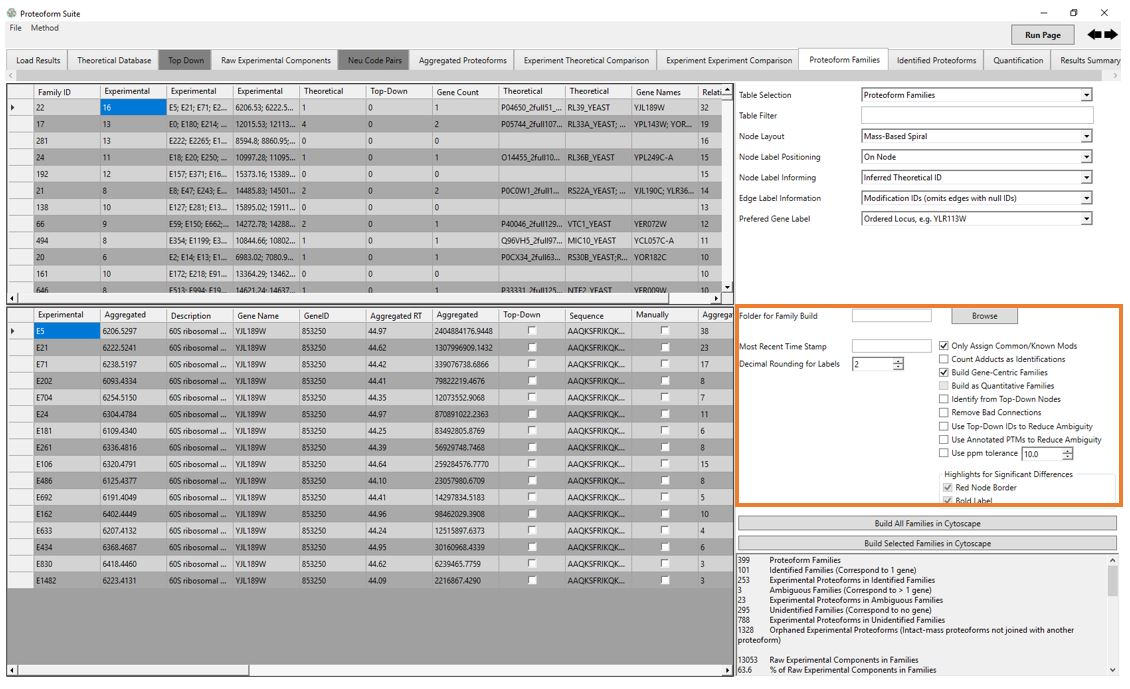
\includegraphics[scale=0.5]{figures/families1.jpg}
\end{figure}
\begin{itemize}
\item Folder for Family Build: folder to build scripts to visualize proteoform families in Cytoscape
\item Most Recent Time Stamp: time stamp that will be in the filename of scripts to visualize proteoform families in Cytoscape
\item Decimal Rounding for Labels: number of decimal places to round labels in visualized proteoform families in Cytoscape
\item Only Assign Common/Known Mods: if checked, intact-mass identifications will only be made for common modifications or for modifications annotated for that theoretical protein in UniProt
\item Count Adducts as Identifications: if checked, adducts (oxidation, sulfate adducts, SDS adducts) will be counted as unique identifications
\item Build Gene-Centric Families: if checked, all proteoforms connected to theoretical proteoforms from the same gene will be grouped into the same proteoform family
\item Build as Quantitative Families: if checked and if quantification was performed, quantitative proteoform families will be built (with pie charts for each experimental proteoform showing abundance ratios)
\item Identify from Top-Down Nodes: if checked, top-down proteoforms in additional to theoretical proteoforms will be used as starting points for identification in proteoform families. This requires high-quality top-down identifications to prevent high false discovery rate
\item Remove Bad Connections: if checked, connections between proteoforms in identified families that do not lead to identification will be removed, unaccepting the experiment-theoretical or experiment-experiment pairs
\item Use Top-Down IDs to Reduce Ambiguity: if checked, top-down IDs will be used to reduce ambiguity in intact-mass identifications; identifications from theoretical proteoforms confirmed by top-down will be prioritized
\item Use Annotated PTMs to Reduce Ambiguity: if checked, annotated PTMs in UniProt will be used to reduce ambiguity in intact-mass identifications; identifications with an annotated PTM will be prioritized
\item Use ppm tolerance: if checked, this ppm tolerance will be used when making intact-mass identifications in proteoform families
\item Highlights for Significant Differences: if checked, a red node border and bold label will be used in quantitative proteoform families to highlight experimental proteoforms with statistically significant quantitative differences
\end{itemize}
\pagebreak
\subsection{Results}
\begin{itemize}
	\item Proteoform Families table: the top table displays all constructed proteoform families
	\begin{figure}[h]
\centering
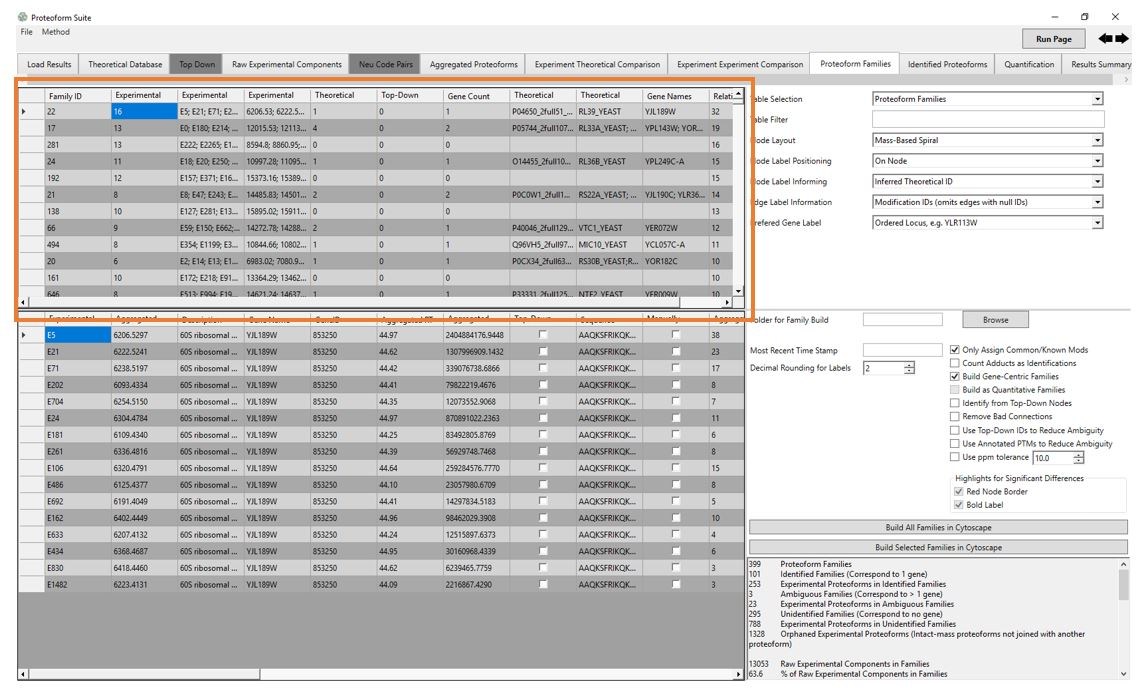
\includegraphics[scale=0.5]{figures/families2.jpg}
\end{figure}
\begin{itemize}
	\item Family ID: unique ID assigned by Proteoform Suite for this proteoform family
	\item Experimental Proteoforms: number of experimental proteoforms in this proteoform family
	\item Experimental Accessions: semi-colon separated list of accessions for experimental proteoforms in this proteoform family
	\item Experimental Aggregated Masses: semi-colon separated list of masses for experimental proteoforms in this proteoform family
	\item Theoretical Proteoforms: number of theoretical proteoforms in this proteoform family
	\item Top-Down Proteoforms: number of top-down proteoforms in this proteoform family
	\item Gene Count: number of genes in this proteoform family. Families with more than 1 gene are ambiguous and families with no genes are unidentified
	\item Theoretical Accessions: semi-colon separated list of accessions for theoretical proteoforms in this proteoform family
	\item Theoretical Names: semi-colon separated list of protein names for this proteoform family
	\item Gene Names: semi-colon separated list of gene names in this proteoform family
	\item Relation Count: number of proteoform relations in this family (experiment-theoretical pairs and experiment-experiment pairs)
\end{itemize}
\item Proteoforms table: the bottom table displays proteoforms for the proteoform family selected in the Proteoform Families table. 
	\begin{figure}[h]
\centering
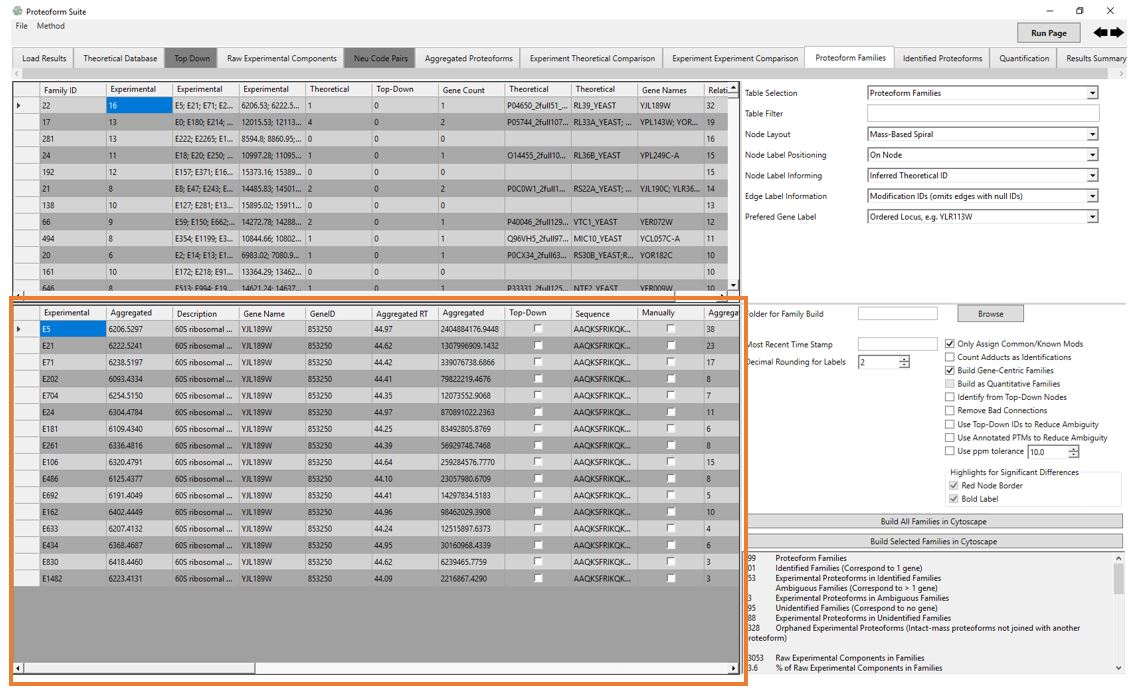
\includegraphics[scale=0.5]{figures/families3.jpg}
\end{figure}
\begin{itemize}
\item If the Experimental Proteoforms, Experimental Accessions, or Experimental Aggregated Masses columns are selected, the experimental proteoforms for the selected family will be displayed. See the Aggregated Proteoforms table in the \textbf{Aggregated Proteoforms} section for column descriptions. 
\item If the Theoretical Proteoforms, Theoretical Accessions, or Theoretical Names Columns are selected, the theoretical proteoforms for the selected family will be displayed. See the Theoretical Proteoforms table in the \textbf{Theoretical Proteoforms} section for column descriptions.
\item If the Top-Down Proteoforms column is selected, the top-down proteoforms for the selected family will be displayed. See the Top-Down Proteoforms table in the \textbf{Top-Down Proteoforms} section for column descriptions.
\item If the Relation Count column is selected, the proteoform relations in the selected family will be displayed. See the Experiment-Theoretical Pairs table in the \textbf{Experiment-Theoretical Comparison} section and the Experiment-Experiment Pairs table in the \textbf{Experiment-Experiment Comparison} section for column descriptions.
\end{itemize}
\item Table Selection: this drop-down box changes which proteoform families are displayed (target or decoy communities). Can also observe theoretical proteoforms and GO Terms
\item Table Filter: filter the Proteoform Families table (top left) by any entered text
\item Node Layout: this drop-down box changes the node layout in visualized proteoform families in Cytoscape
\item Node Label Positioning: this drop-down box changes the position of node labels in visualized proteoform families in Cytoscape
\item Node Label Informing: this drop-down box changes the node label information in visualized proteoform families in Cytoscape
\item Edge Label Information: this drop-down box changes the edge label information in visualized proteoform families in Cytoscape
\item Preferred Gene Label: this drop-down box changes the gene label information in visualized proteoform families in Cytoscape
\item Build All Families in Cytoscape: exports scripts for Cytoscape to visualize all proteoform families
\item Build Selected Families in Cytoscape: exports scripts for Cytsocape to visualize proteoform families selected in the Proteoform Families table
\item The text box at the bottom right of the page displays information about the results. See the \textbf{Results Summary} section for a description of each result
\end{itemize}
\pagebreak
%!TEX root = ../proteoform_suite_manual.tex
%---------------------------------------------------------------------
%	CYTOSCAPE VISUALIZATION
%---------------------------------------------------------------------

\section{Visualizing Proteoform Families in Cytoscape}

\subsection{Overview}
Proteoform families are visualized in the software program Cytoscape.\supercite{Shannon2003,Smoot2011} Each node is a proteoform and each edge represents a mass difference between proteoforms, corresponding to a modification or amino acid difference. Proteoform family visualization allows users to visualize all observed proteoforms and modification combinations from each family in a simple graphic. Install Cytoscape version 3.5.0: \url{https://cytoscape.org/download.html}.


\subsection{Visualize Families in Cytoscape}
\begin{itemize}
	\item Export scripts for Cytoscape either on the Proteoform Families page or the Results Summary page
	\begin{itemize}
		\item Cytoscape\_style\_timestamp: file Cytoscape uses to correctly style visualized proteoform families
		\item Cytoscape\_nodes\_timestamp: file containing node information for visualized proteoform families
		\item Cytoscape\_edges\_timestamp: file containing edge information for visualized proteoform families
		\item Cytoscape\_script\_timestamp: script for Cytoscape to load in the style, nodes, and edges file and visualize proteoform families
	\end{itemize}
	\item In Cytoscape, select Tools $>$ Execute Command File.... 
	\item Select the cytoscape\_script\_timestamp file generated by Proteoform Suite
	\item Proteoform families will appear! Should take about 1 min for larger proteoform families.
\end{itemize}
\begin{figure}[h]
\centering
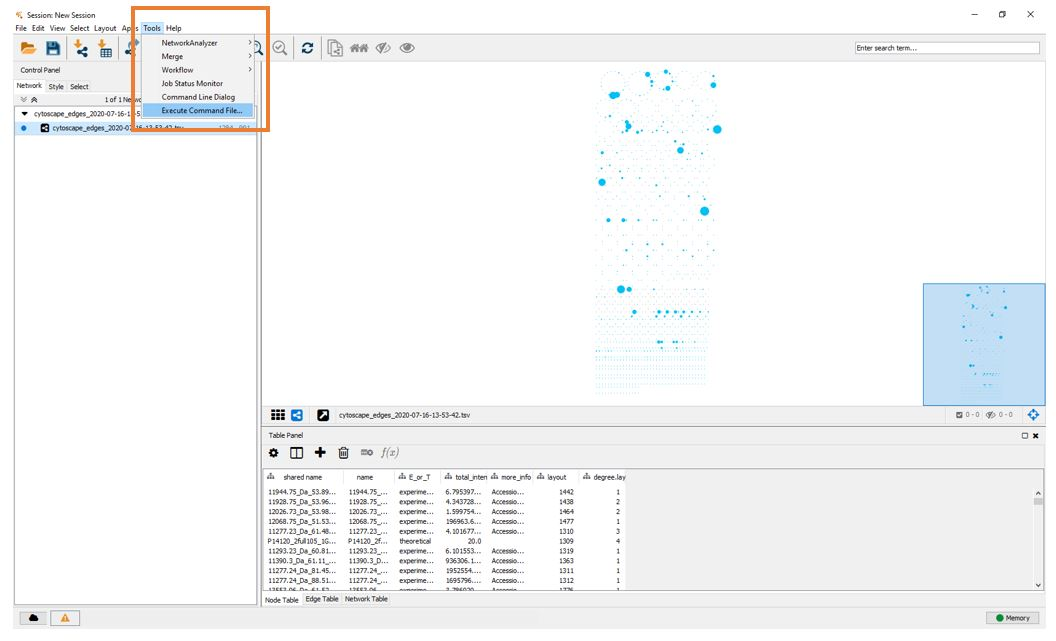
\includegraphics[scale=0.45]{figures/cytoscape1.jpg}
\end{figure}

\pagebreak
\subsection{Proteoform Families Key}
\begin{itemize}
	\item Pink square: gene name
	\item Green nodes: theoretical proteoforms
	\item Blue nodes: experimental proteoforms; size of node is proportional to summed intensity
	\item Purple nodes: top-down proteoforms
	\item Edges: mass differences between proteoforms
	\item Specialized
	\begin{itemize}
		\item Quantified Proteoform families: pie chart for each experimental proteoform shows abundance ratio between two conditions (blue and yellow)
		\item Bottom-up data: orange nodes are bottom-up peptides. Edges indicate that the peptide could be derived from connected the proteoform node
	\end{itemize}
\end{itemize}
\begin{figure}[h]
\centering
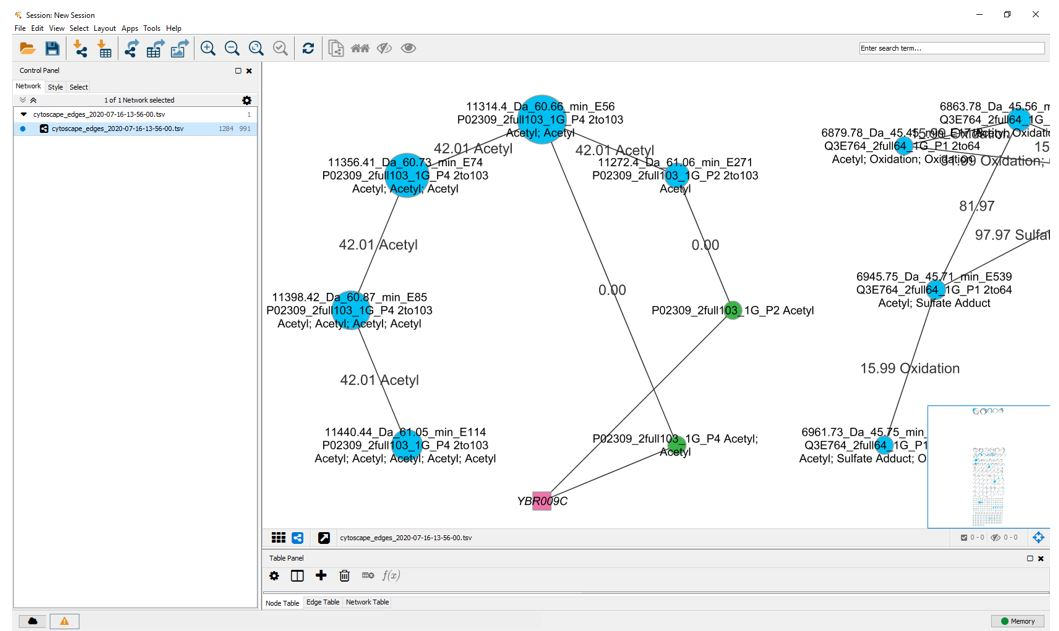
\includegraphics[scale=0.5]{figures/cytoscape2.jpg}
\end{figure}

\subsection{Exporting Family Visualizations into Adobe Illustrator}
\begin{itemize}
	\item In Cytoscape, File $>$ Export $>$ Network View as Graphics...
	\item Select SVG
	\item This will export everything in view into a format that can be loaded by Adobe Illustrator and polished there for publication
\end{itemize}




\pagebreak
%!TEX root = ../proteoform_suite_manual.tex
%---------------------------------------------------------------------
%	IDENTIFIED PROTEOFORMS
%---------------------------------------------------------------------

\section{Identified Proteoforms}


\subsection{Overview}

On this page, all identified proteoforms are displayed, including intact-mass identification (from proteoform family construction) and top-down identifications (from loaded top-down results). The results automatically refresh each time the page is loaded. 

\subsection{Results}
\begin{itemize}
	\item Compare With other Top-Down Results: option to select another top-down hit results file and export and Excel file comparing intact-mass identifications with top-down identifications
	\item Table Filters: filter Identified Intact-Mass Experimental Proteoforms table (top left) and Top-Down Proteoforms table (top right) by any entered text
	\item Identified Intact-Mass Experimental Proteoforms: the left table displays experimental proteoforms identified by intact-mass analysis (proteoform family construction).  See the Aggregated Proteoforms table in the \textbf{Aggregated Proteoforms} section for column descriptions. 
	\begin{figure}[h]
\centering
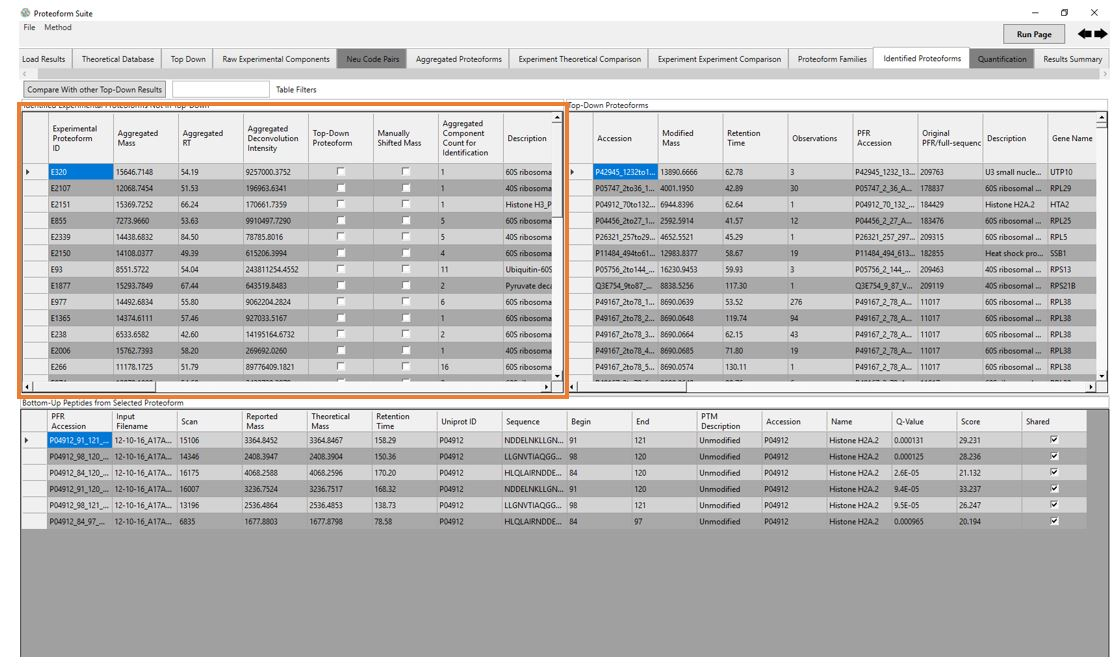
\includegraphics[scale=0.45]{figures/identified1.jpg}
\end{figure}
\pagebreak
\item Top-Down Proteoforms: the right table displays top-down proteoform identifications (aggregated from top-down hit results loaded from top-down results). See the Top-Down Proteoforms table in the \textbf{Top-Down Proteoforms} section for column descriptions.
	\begin{figure}[h]
\centering
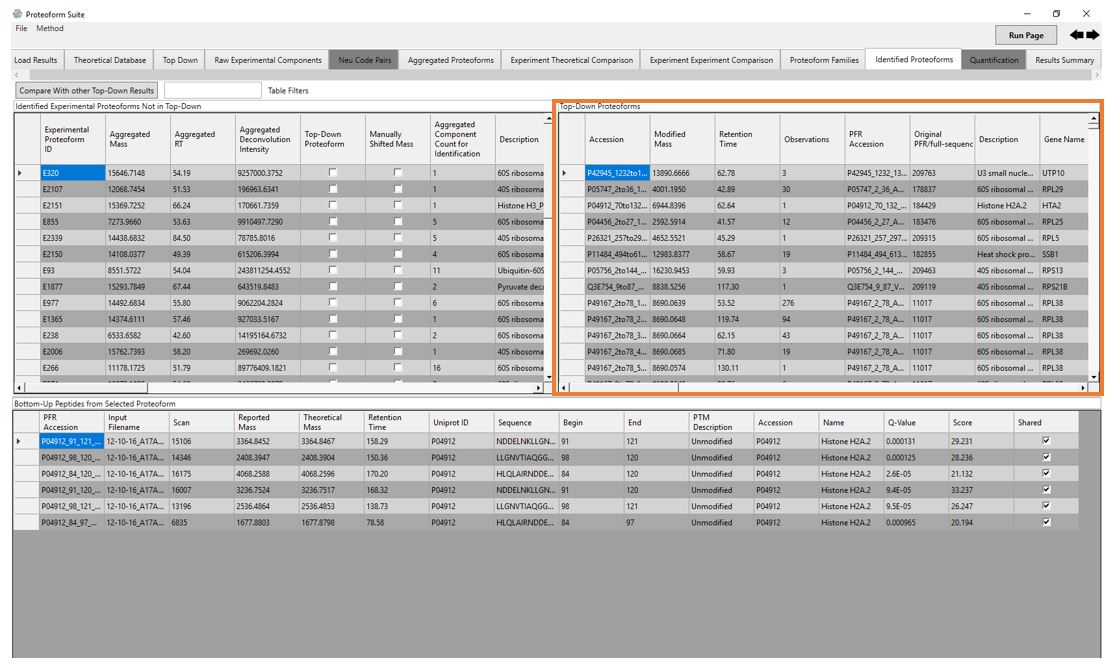
\includegraphics[scale=0.45]{figures/identified2.jpg}
\end{figure}
\item Bottom-Up Peptides from Selected Proteoform: the bottom table displays bottom-up peptides from the selected proteoform in either the Identified Intact-Mass Experimental Proteoforms table or the Top-Down Proteoforms table. See the Bottom-Up Peptides table in the \textbf{Top-Down Proteoforms} section for column descriptions.
	\begin{figure}[h]
\centering
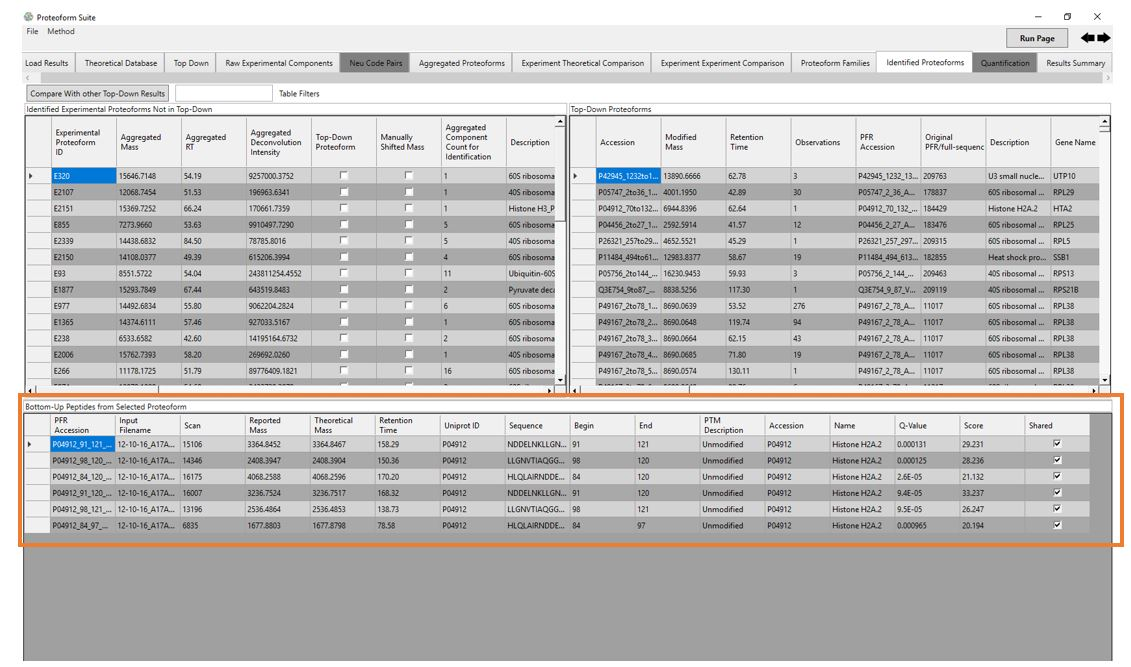
\includegraphics[scale=0.45]{figures/identified3.jpg}
\end{figure}
\end{itemize}
\pagebreak
%!TEX root = ../proteoform_suite_manual.tex
%---------------------------------------------------------------------
%	QUANTIFICATION
%---------------------------------------------------------------------

\section{Quantification}

\subsection{Overview}
On this page, experimental proteoforms are quantified and Proteoform Suite determines experimental proteoforms with statistically significant abundance differences between two conditions. Two separate statistical tests are performed: a permutation analysis based on Tusher et al.\supercite{Tusher2001} and a log2 fold-change t-test with a Benjamini Hochberg multiple testing correction. 

\subsection{Run Page}
\begin{itemize}
\item The Proteoform Families page must be run before running this page.
\item Set all parameters as desired for current analysis (see below)
\item Click Run Page button (top right)
\end{itemize}

\subsection{Set Parameters}
\begin{figure}[h]
\centering
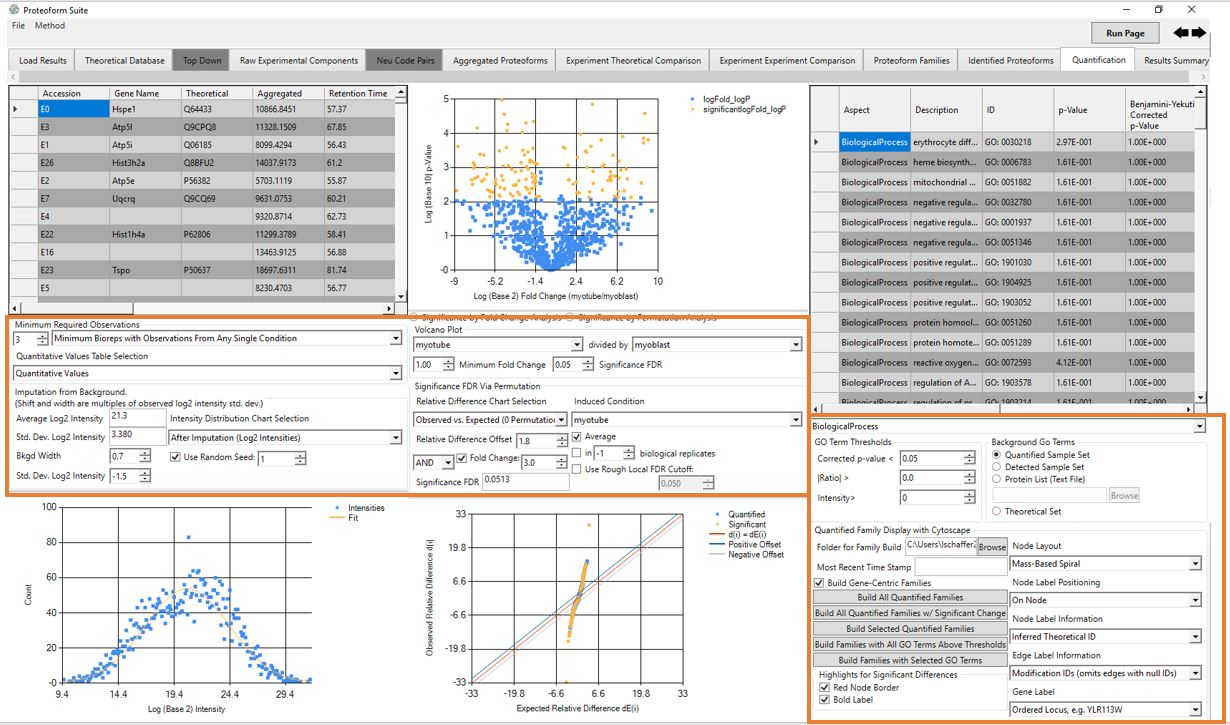
\includegraphics[scale=0.43]{figures/quant1.jpg}
\end{figure}
\begin{itemize}
\item Minimum Required Observations: set the \# (left) and the requirement (right drop down box) to require quantitative observations of an experimental proteoform in more than one file type
\item Quantitative Values Table Selection: select what will be displayed in the Quantitative Values table (top right)
\item Bkgd Width: background distribution for imputation width (sigma)
\item Std. Dev. Log2 Intensity: background distribution for imputation shift, number of sigma from the population mean
\item Use Random Seed: a random seed will be used in the random number generator for selecting imputed intensity values, resulting in the same intensity values each time (with the same given parameters)
\item Significant by Fold Change Analysis: select this option to have the fold change analysis be what determines which experimental proteoforms have statistically significant abundance changes
\item Significance by Perutations: select this option to have the permutation analysis be what determines which experimental proteoforms have statistically significant abundance changes
\item Volcano Plot: choose which condition intensity is divided by which condition intensity
\item Minimum Fold Change: set the minimum log2 fold change for an experimental proteoform's abundance change to be considered significant
\item Significance FDR: set the maximum false discovery rate for an experimental proteoform's abundance change to be considered statistically significant
\item Relative Difference Chart Selection: select which permutation analysis chart is displayed in the bottom middle graph
\item Induced Condition: select which condition is the induced condition
\item Relative Difference Offset: select a minimum relative difference offset from the expected relative difference curve for an abundance change to be considered significant using permutation analysis
\item AND/OR: option to use both relative difference offset and/or a minimum fold change value
\item Fold Change: select a minimum fold change value for an abundance change to be considered significant
\item Average: check this box to use average permutation fold change
\item In \# biological replicates: check this box and set the \# to set a minimum number of biological replicates
\item Use Rough Local FDR cutoff: check this box to use a local false discovery rate cutoff in permutation analysis; set the maximum FDR cutoff below
\item GO Term Dropbox: select which gene ontology terms to display in the Gene Ontology table (top right)
\item GO Term Thresholds: select thresholds for a gene ontology term to be considered significant (maximum p-value, minimum ratio, minimum intensity)
\item Background GO Terms: select what should be used for the background gene ontology terms (quantified only, all detected, or a new protein list loaded in with Browse)
\end{itemize}
\pagebreak
\subsection{Results}
\begin{itemize}
\item Quantitative Values table: this top left table displays quantified experimental proteoforms
\begin{figure}[h]
\centering
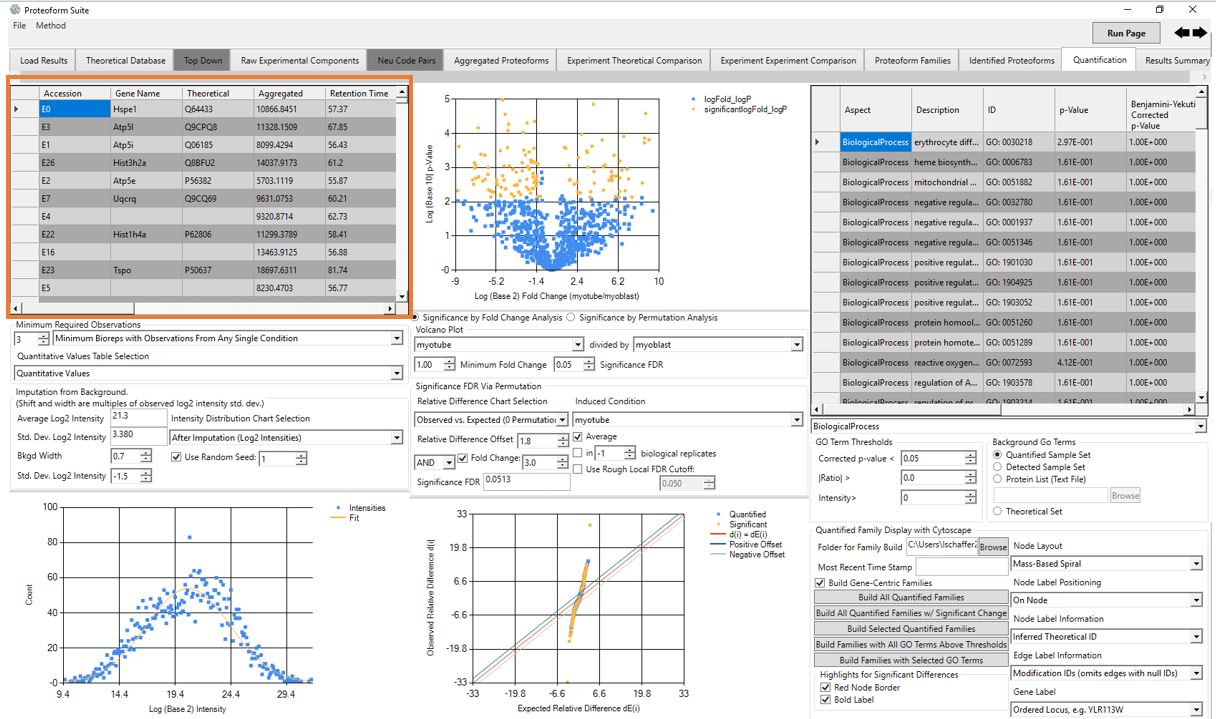
\includegraphics[scale=0.43]{figures/quant2.jpg}
\end{figure}
\begin{itemize}
	\item Accession: unique accession given by Proteoform Suite given to this experimental proteoform
	\item Gene Name: if identified, gene name for this experimental proteoform
	\item Theoretical: if identified, theoretical accession from UniProt for this experimental proteoform
	\item Aggregated Mass: monoisotopic mass of experimental proteoform, weighted average of (light) raw experimental components by intensity
	\item Aggregated RT: retention time of experimental proteoform, average of raw experimental components (unlabeled) or NeuCode pairs (NeuCode labeled)
	\item Condition1 Intensity Sum: summed intensity of raw quantitative components for this condition for this experimental proteoform
	\item Condition2 Intensity Sum: summed intensity of raw quantitative components for this condition for this experimental proteoform
	\item Intensity Sum: total summed intensity of all raw quantitative components (both conditions) for this experimental proteoform
	\item Log2 Fold Change: log2 fold change between 2 conditions for this experimental proteoform
	\item Scatter linear: if significance by permutation analysis, linear intensity
	\item p-value: if significance by fold change analysis, p-value for this experimental proteoform fold change test statistic
	\item Benjamini-Hochberg corrected p-value: if significance by fold change analysis, Benjamini-Hochberg corrected p-value for this experimental proteoform fold change test statistic
	\item Significant: checked if fold change for this experimental proteoform is statistically significant
	\item Student's t-test Statistic: test statistic for log2 fold change analysis t-test
	\item Corresponding Avg. Permuted Student's t-Test Statistic: averaged permuted student's test statistic
	\item Manual Validation: file information for manual validation of most abundant raw quantitative component 
\end{itemize}
\item Imputations from Background: this bottom left graph displays info about the log2 intensities of quantified proteoforms, with an option to view before and after imputation. 
\begin{figure}[h]
\centering
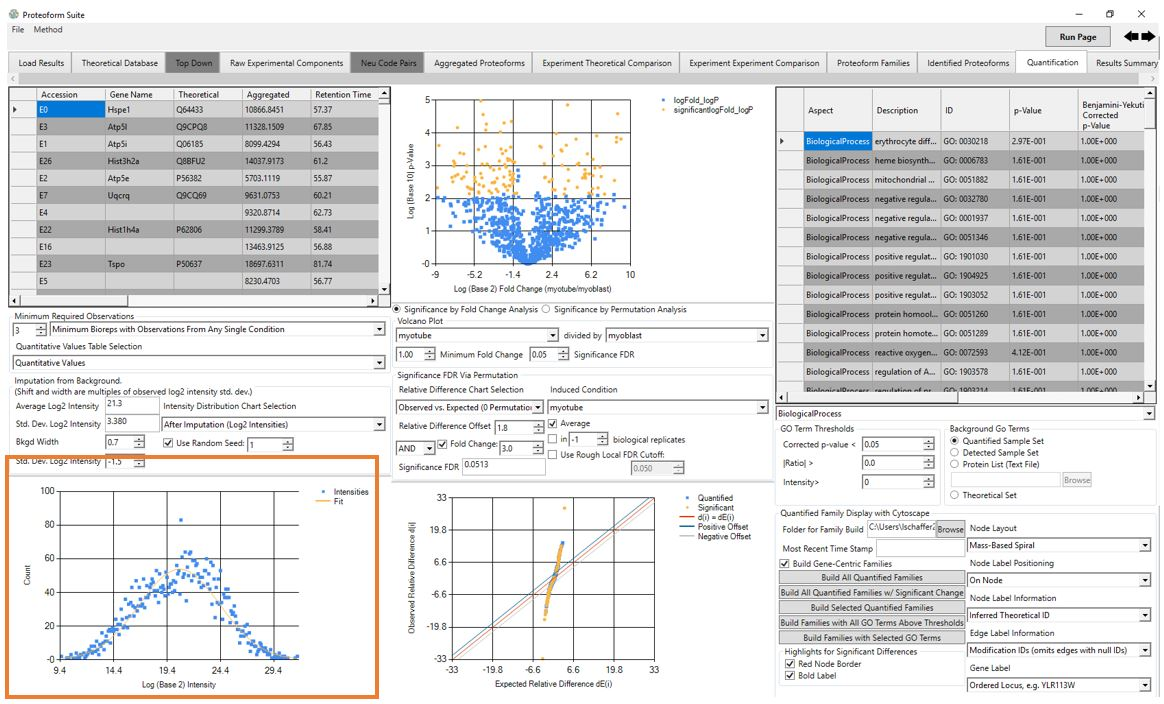
\includegraphics[scale=0.43]{figures/quant3.jpg}
\end{figure}
\pagebreak
\item Volcano plot: this top middle graph shows the a volcano plot from the fold change analysis, p-value vs. log2 fold change. Proteoforms with a statistically significant fold change are yellow, other proteoforms are blue.
\begin{figure}[h]
\centering
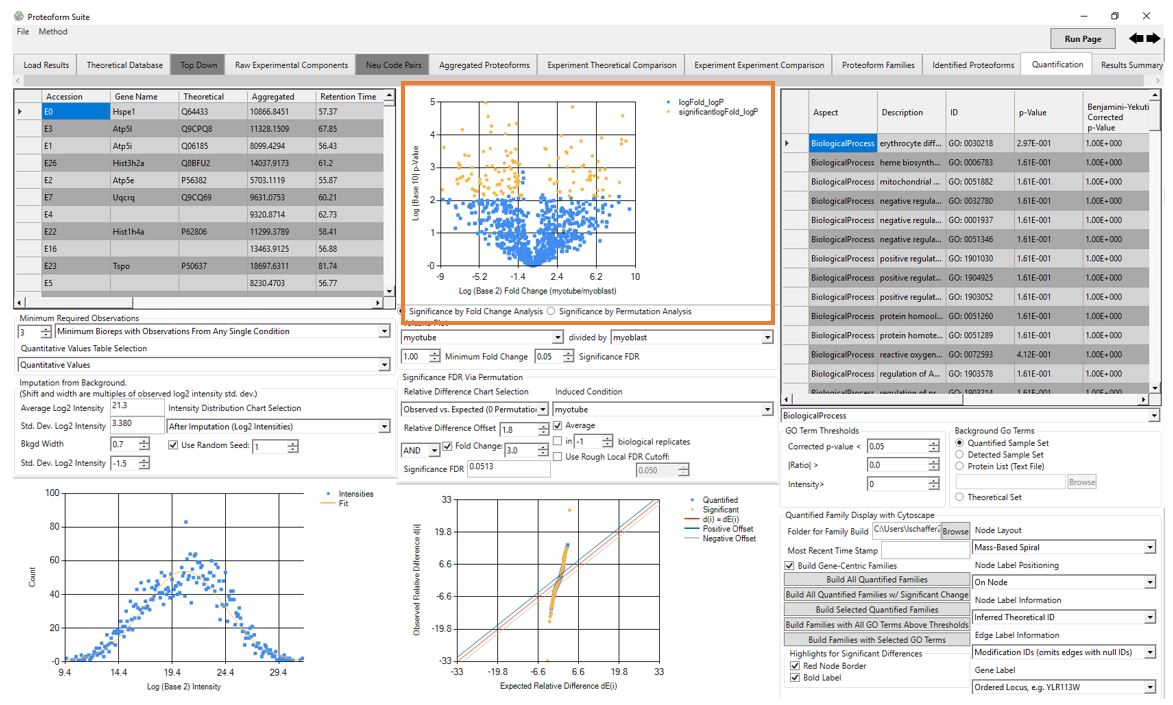
\includegraphics[scale=0.43]{figures/quant4.jpg}
\end{figure}
\item Permutation Analysis graph: the bottom middle graph shows information from the permutation analysis, including observed relative difference vs. expected relative difference
\begin{figure}[h]
\centering
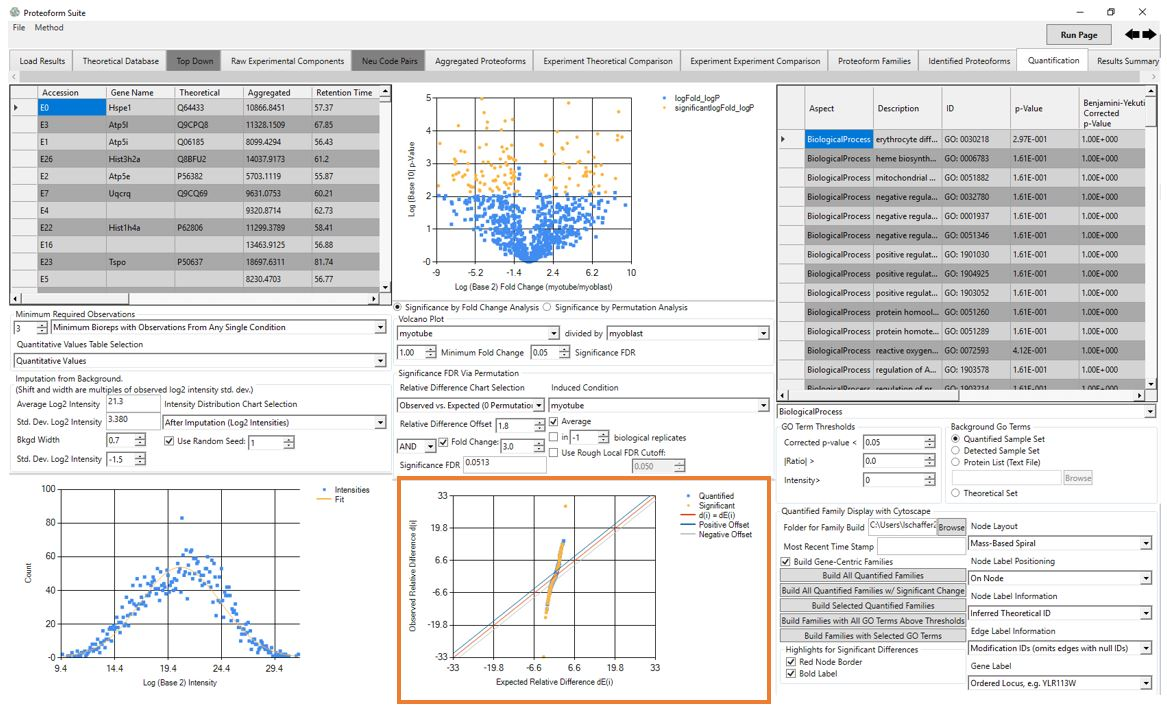
\includegraphics[scale=0.43]{figures/quant5.jpg}
\end{figure}
\item Gene Ontology Terms table: the top right table displays the gene ontology terms
\begin{figure}[h]
\centering
\includegraphics[scale=0.43]{figures/quant6.jpg}
\end{figure}
\begin{itemize}
\item Aspect: gene ontology term type
\item Description: gene ontology term description
\item ID: gene ontology term
\item P-Value: p-value for this gene ontology term
\item Benjamini-Yekutieli Corrected p-Value: Benjamini-Yekutieli corrected p-value for this gene ontology term
\item Log Odds Ratio: log odds ratio
\item Significant Proteins With This Go-Term: number of unique proteins with this GO term and with an experimental proteoform with a statistically significant abundance change
\item Total Significant Proteins: number of unique proteins with an experimental proteoform with a statistically significant abundance change
\item Background Proteins With This Go-Term: number of unique background proteins with this GO term
\item Total Background Proteins: total number of background proteins
\end{itemize}
\item Folder for Family Build: folder to build scripts to visualize proteoform families in Cytoscape
\item Most Recent Time Stamp: time stamp that will be in the filename of scripts to visualize proteoform families in Cytoscape
\item Build Gene-Centric Families: if checked, all proteoforms connected to theoretical proteoforms from the same gene will be grouped into the same proteoform family
\item Build All Quantified Families: exports scripts for Cytoscape to visualize all quantified proteoform families
\item Build All Quantified Families w/ Significant Change: exports scripts for Cytoscape to visualize all quantified proteoform families with at least one experimental proteoform with a statistically significant abundance change
\item Build Selected Quantified Families: exports scripts for Cytsocape to visualize proteoform families with an experimental proteoform selected in the Quantification Values table
\item Build Families with All GO Terms Above Threshold: exports scripts for Cytoscape to visualize all quantified proteoform families with gene ontology terms above threshold
\item Build Families with Selected GO Terms: exports scripts for Cytoscape to visualize proteoform families with a gene ontology term selected in the Gene Ontology Terms table
\item Highlights for Significant Differences: if checked, a red node border and bold label will be used in quantitative proteoform families to highlight experimental proteoforms with statistically significant quantitative differences
\item Node Layout: this drop-down box changes the node layout in visualized proteoform families in Cytoscape
\item Node Label Positioning: this drop-down box changes the position of node labels in visualized proteoform families in Cytoscape
\item Node Label Informing: this drop-down box changes the node label information in visualized proteoform families in Cytoscape
\item Edge Label Information: this drop-down box changes the edge label information in visualized proteoform families in Cytoscape
\item Preferred Gene Label: this drop-down box changes the gene label information in visualized proteoform families in Cytoscape
\end{itemize}
\pagebreak
%!TEX root = ../proteoform_suite_manual.tex
%---------------------------------------------------------------------
%	RESULTS
%---------------------------------------------------------------------

\section{Results Summary}

\subsection{Overview}
This page displays all of the results from the Proteoform Suite analysis. The results automatically refresh each time the page is loaded. Results and tables can be exported.

\subsection{Results}
\begin{itemize}
\item Results Folder: browse for a folder where all results will be exported
\item Save All: save all results files in the folder selected
\begin{itemize}
\item ExperimentExperimental\_MassDifferences\_timestamp.png: image of Experiment-Experiment Delta Mass Histogram
\item ExperimentTheoretical\_MassDifferences\_timestamp.png: image of Experiment-Theoretical Delta Mass Histogram
\item Presets\_timestamp.xml: method file of all set parameters in Proteoform Suite. Can be used in future Proteoform Suite analyses to replicate this analysis
\item Proteoform\_bottomup\_evidence\_timestamp.tsv: if bottom-up data input, this is a list of potential proteoforms inferred with bottom-up evidence
\item Bottomup\_results\_timestampe.tsv: if bottom-up data input, this is a list of bottom-up peptides
\item Shared\_peptide\_bottomup\_results\_timestamp.tsv: if bottom-up data input, this is a list of shared bottom-up peptides
\item Topdown\_results\_timestampe.tsv: if top-down data input, this is a list of top-down proteoforms
\item AllFamilies\_cytoscape\_edges\_timestamp.tsv: file containing edge information for all proteoform families in Cytoscape visualization
\item AllFamilies\_cytoscape\_nodes\_timestamp.tsv: file containing node information for all proteoform families in Cytoscape visualization
\item AllFamilies\_cytoscape\_script\_timestamp.tsv: script to visualize all proteoform families in Cytoscape
\item AllFamilies\_cytoscape\_style\_timestamp.tsv: file containing style information for all proteoform families in Cytoscape visualization
\item BottomUp\_cytoscape\_edges\_timestamp.tsv: if bottom-up data input, file containing edge information for all proteoform families in Cytoscape visualization
\item BottomUp\_cytoscape\_nodes\_timestamp.tsv: if bottom-up data input, file containing node information for all proteoform families in Cytoscape visualization
\item BottomUp\_cytoscape\_script\_timestamp.tsv: if bottom-up data input, script to visualize peptide-to-proteoform relations in Cytoscape
\item BottomUp\_cytoscape\_style\_timestamp.tsv: if bottom-up data input, file containing style information for all proteoform families in Cytoscape visualization
\item Decoy\_experimental\_results\_timestamp.tsv: all decoy intact-mass identifications
\item Experimental\_intensities\_by\_file\_timestampe.tsv: intensity for each file for each experimental proteoform
\item Experimental\_results\_timestamp.tsv: experimental proteoform intact-mass identifications
\item Summary\_timestampe.txt: summary of all proteoform results, displayed on Results Summary page
\end{itemize}
\item Results Summary
\begin{itemize}
\item Unprocessed Raw Experimental Components: the number of raw experimental components for identification before merging artifacts
\item Raw Experimental Components:  the number of raw experimental components for identification after merging artifacts
\item Missed Monoisotopic Raw Experimental Components Merged: the number of raw experimental components for identification artifacts merged due to being missed monoisotopic errors within the set mass tolerance
\item Harmonic Raw Experimental Components Merged: the number of raw experimental components for identification artifacts merged due to being charge state harmonic errors within the set mass tolerance
\item Unprocessed Raw Quantitative Components: the number of raw experimental components for quantification before merging artifacts
\item Raw Quantitative Components: the number of raw experimental components for quantification after merging artifacts
\item Missed Monoisotopic Raw Quantitative Components Merged: the number of raw experimental components for quantification artifacts merged due to being missed monoisotopic errors within the set mass tolerance
\item Harmonic Raw Quantitative Components Merged: the number of raw experimental components for quantification artifacts merged due to being charge state harmonic errors within the set mass tolerance
\item Raw NeuCode Pairs: the total number of NeuCode pairs, each with a heavy and light NeuCode raw experimental component 
\item Accepted NeuCode Pairs: the number of accepted NeuCode pairs, which are used in subsequent analysis
\item Top-Down Hit: total number of top-down hits (proteoform spectral matches)
\item Accepted Top-Down Proteoforms: number of aggregated top-down proteoforms. May be greater than the number of unique PFRs if some hits of the same ID fall outside of the retention time tolerance
\item Experimental Proteoforms: the total number of experimental proteoforms
\item Accepted Experimental Proteoforms: the number of accepted experimental proteoforms that are used in subsequent analysis
\item Accepted Intact-Mass Experimental Proteoforms: the number of accepted experimental proteoforms aggregated from raw experimental components from deconvolution results
\item Accepted Top-Down Experimental Proteoforms: the number of accepted experimental proteoforms aggregated from top-down hits from top-down results
\item Theoretical Proteins: the number of unique proteins
\item Expanded Theoretical Proteins: the number of unique protein sequences, including annotated subsequences
\item Theoretical Proteoforms: the number of theoretical proteoforms in the database
\item Experimental-Theoretical Peaks: the total number of experiment-theoretical delta mass peaks
\item Experimental-Theoretical Pairs: the total number of experiment-theoretical pairs, each with a delta mass between the experiment and theoretical proteoforms
\item Accepted Experimental-Theoretical Peaks: the number of accepted experiment-theoretical delta mass peaks
\item Accepted Experimental-Theoretical Pairs: the number of experiment-theoretical pairs in accepted delta mass peaks, used in subsequent proteoform family construction
\item Average Experimental-Decoy Pairs: the average number of experiment-decoy pairs across all decoy databases generated
\item Experimental-Experimental Peaks: the total number of experiment-experiment delta mass peaks
\item Experimental-Experimental Pairs: the total number of experiment-experiment pairs, each with a delta mass between the two experimental proteoforms
\item Accepted Experimental-Experimental Peaks: the number of accepted experiment-experiment delta mass peaks
\item Accepted Experimental-Experimental Pairs: the number of experiment-experiment pairs in accepted delta mass peaks, used in subsequent proteoform family construction
\item Average Experimental-False Pairs: the average number of experiment-false pairs across all decoy analyses
\item Proteoform Families: the number of constructed proteoform families, from accepted experiment-theoretical and experiment-experiment pairs
\item Identified Families (Correspond to 1 gene): the number of proteoform families with one unique gene from the theoretical proteoforms in the family
\item Experimental Proteoforms in Identified Families: the number of experimental proteoforms in identified proteoform families with 1 gene
\item Ambiguous Families (Correspond to $>$ 1 gene): the number of proteoform families with more than one unique gene from the theoretical proteoforms in the family
\item Experimental Proteoforms in Ambiguous Families: the number of experimental proteoforms in ambiguous proteoform families with more than 1 gene
\item Unidentified Families (Correspond to no gene): the number of proteoform families with no genes (no theoretical proteoforms)
\item Experimental Proteoforms in Unidentified Families: the number of experimental proteoforms in unidentified families with no theoretical proteoforms/genes
\item Orphaned Experimental Proteoforms (Intact-mass proteoforms not joined with another proteoform): the number of experimental proteoforms that were not part of any accepted experiment-theoretical or experiment-experiment pairs
\item Raw Experimental Components in Families: the number of raw experimental components that were aggregated into an experimental proteoform that was a part of a proteoform family (non-orphans)
\item \% of Raw Experimental Components in Families: the percentage of raw experimental components that were aggregated into an experimental proteoform that was a part of a proteoform family (non-orphans)
\item Raw Quantitative Components in Families: the number of raw quantitative components that were aggregated into an experimental proteoform that was a part of a proteoform family (non-orphans)
\item \% of Raw Quantitative Components in Families:  the percentage of raw quantitative components that were aggregated into an experimental proteoform that was a part of a proteoform family (non-orphans)
\item Identified Experimental Proteoforms: the number of experimental proteoforms that were identified from proteoform family construction of experiment-theoretical and experiment-experiment pairs
\item Average Identified Experimental Proteoforms by Decoys: the average number of experimental proteoforms that were identified from proteoform family construction of experiment-decoy and experiment-false pairs
\item Proteoform FDR: the calculated global false discovery rate (average number of decoy identifications / experimental proteoform identifications)
\item Identified Experimental Proteoforms (no Ambiguous): the number of experimental proteoforms that were identified from proteoform family construction of experiment-theoretical and experiment-experiment pairs, excluding ambiguous identifications
\item Average Identified Experimental Proteoforms by Decoys (no Ambiguous): the average number of experimental proteoforms that were identified from proteoform family construction of experiment-decoy and experiment-false pairs, excluding ambiguous identifications
\item Proteoform FDR:  the calculated global false discovery rate (average number of decoy identifications / experimental proteoform identifications), excluding ambiguous identifications
\item Top-Down Proteoforms Assigned Same Identification by Intact-Mass Analysis: the number of top-down proteoforms that were assigned the same identification through proteoform family construction as the original top-down identification
\item Top-Down Proteoforms Assigned Different Identification by Intact-Mass Analysis: the number of top-down proteoforms that were assigned a different identification through proteoform family construction as the original top-down identification
\item Top-Down Proteoforms Assigned Amibguous Identification by Intact-Mass Analysis: the number of top-down proteoforms that were assigned an ambiguous identification through proteoform family construction
\item Top-Down Proteoforms Unidentified by Intact-Mass Analysis: the number of top-down proteoforms that were not assigned an identification through proteoform family construction
\item Unique Top-Down Protein Identifications (TDPortal): then umber of unique protein identifications from the top-down identifications
\item Total Unique Protein Identifications: the total number of unique protein identifications, top-down + intact-mass
\item Unique Intact-Mass Experimental Proteoform Identifications: the total number of unique protein identifications from proteoform family construction
\item Ambiguous Intact-Mass Experimental Proteoform Identifications: the number of ambiguous experimental proteoform identification from proteoform family construction
\item Unique Top-Down Proteoforms Identifications (TDPortal): the number of unique top-down proteoform identifications from the top-down hit results
\item Unidentified Intact-Mass Experimental Proteoforms: the number of unidentified intact-mass experimental proteoforms (aggregated from raw experimental components from deconvolution results)
\item Total Unique Proteoform Identifications: the total number of unique proteoform identifications from top-down results and intact-mass results
\item Quantified Experimental Proteoforms (Threshold for Quantification: 0 = Minimum Bioreps with Observations From Any Single Condition): the number of experimental proteoforms that met the minimum threshold for quantification analysis
\item Average Log2 Intensity Quantified Experimental Proteoform Observations: the average log2 intensity of experimental proteoforms that were quantified (calculated from the raw quantitative components)
\item Log2 Intensity Standard Deviation for Quantified Experimental Proteoform: the standard deviation fo the log2 intensity of experimental proteoforms that were quantified
\item Experimental Proteoforms with Significant Change (Threshold for Significance: Log2FoldChange $>$ 0, \& Total Intensity from Quantification $>$ 0, \& Q-Value $<$ 0.05): experimental proteoforms with statistically significant fold change from both relative difference and fold change analysis
\item Experimental Proteoforms with Significant Change by Relative Difference (Offset of 1 from d(i) = dE(i) line): number of proteoforms with statistically significant relative difference in Tusher analysis with X permutations
\item Experimental Proteoforms with Significant Change by Fold Change (Offset of 1 from d(i) = dE(i) line): number of proteoforms with statistically significant fold change in Tusher analysis with X permutations
\item FDR for Significance Conclusion (Offset of 1 from d(i) = dE(i) line): the false discovery rate for the relative difference analysis from the Tusher analysis with X permutations
\item Proteoform Families with Significant Change: number of proteoform families with at least one experimental proteoform with a statistically significant fold change from the Tusher analysis with X permutations
\item Identified Proteins with Significant Change: the number of unique identified proteins with at least one identified experimental proteoform with a statistically significant fold change from the Tusher analysis with X permutations
\item GO Terms of Significance (Benjimini-Yekeulti p-value $<$ 0.05; using Experimental Proteoforms that satisified the criteria:  Log2FoldChange $>$ 0, \& Total Intensity from Quantification $>$ 0, \& Q-Value $<$ 0.05): number of significant gene ontology terms from the Tusher analysis with X permutations
\item Experimental Proteoforms with Significant Change (Threshold for Significance: Benjimini-Hochberg Q-Value $<$ 0.05): number of proteoforms with statistically significant fold change from log2 fold change t-test with Benjamini-Hochberg correction
\item FDR for Significance Conclusion: FDR value for fold change to be considered statistically significant
\item Proteoform Families with Significant Change: number of proteoforms with statistically significant  relative difference from log2 fold change t-test with Benjamini-Hochberg correction
\item Identified Proteins with Significant Change: the number of unique identified proteins with at least one identified experimental proteoform with a statistically significant fold change from log2 fold change t-test with Benjamini-Hochberg correction
\item GO Terms of Significance (Benjimini-Yekeulti p-value $<$ 0.05; using Experimental Proteoforms that satisified the criteria:  Log2FoldChange $>$ 0, \& Total Intensity from 
\item Quantification $>$ 0, \& Q-Value $<$ 0.05): number of significant gene ontology terms from log2 fold change t-test with Benjamini-Hochberg correction
\item Identified Proteins with Significant Change: (0 Permutations): list of unique identified proteins with at least one identified experimental proteoform with a statistically significant fold change from Tusher analysis with X permutations
\item Identified Proteins with Significant Change: (by log2 fold change analysis): list of unique identified proteins with at least one identified experimental proteoform with a statistically significant fold change from log2 fold change t-test with Benjamini-Hochberg correction
\item GO Terms of Significance, Tusher Analysis with 0 permutations (Benjimini-Yekeulti p-value $<$ 0.05): list of statistically significant gene ontology terms from Tusher analysis with X permutations
\item GO Terms of Significance, Log2 Fold Change Analysis with 0.05 FDR (Benjimini-Yekeulti p-value $<$ 0.05): list of statistically significant gene ontology terms from log2 fold change t-test with Benjamini-Hochberg correction
\item USER ACTIONS: list of user actions, including adding files, changing file labels, accepting/unaccepting delta mass peaks, shifting the mass of experiment-theoretical delta mass peaks
\item DECONVOLUTION RESULTS FILES AND PROTEIN DATABASE FILES: list of files loaded on the Load Results page
\end{itemize}
\end{itemize}


\pagebreak
%\input{docs/glossary}

% References ------------------------------------------------------
\pagebreak
\addcontentsline{toc}{section}{References}
\printbibliography

\end{document}
